%----------------------------------------------------------------------------------------
%	PACKAGES AND OTHER DOCUMENT CONFIGURATIONS
%----------------------------------------------------------------------------------------

\documentclass[
11pt, % The default document font size, options: 10pt, 11pt, 12pt
%oneside,% Two side (alternating margins) for binding by default, uncomment to switch to one side
twoside,
english, % ngerman for German
singlespacing, % Single line spacing, alternatives: onehalfspacing or doublespacing
%draft, % Uncomment to enable draft mode (no pictures, no links, overfull hboxes indicated)
%nolistspacing, % If the document is onehalfspacing or doublespacing, uncomment this to set spacing in lists to single
%liststotoc, % Uncomment to add the list of figures/tables/etc to the table of contents
%toctotoc, % Uncomment to add the main table of contents to the table of contents
%parskip, % Uncomment to add space between paragraphs
%nohyperref, % Uncomment to not load the hyperref package
headsepline, % Uncomment to get a line under the header
%chapterinoneline, % Uncomment to place the chapter title next to the number on one line
%consistentlayout, % Uncomment to change the layout of the declaration, abstract and acknowledgements pages to match the default layout
]{config/ThesisPreamble} % The class file specifying the document structure

\usepackage[utf8]{inputenc} % Required for inputting international characters
\usepackage[T1]{fontenc} % Output font encoding for international characters

%\usepackage{mathpazo} % Use the Palatino font by default

\usepackage[backend=bibtex,style=numeric,sorting=none]{biblatex} % Use the bibtex backend with the authoryear citation style (which resembles APA)

\addbibresource{config/references.bib} % The filename of the bibliography

\usepackage{tikz}
\usepackage{pgfplots}
\pgfplotsset{compat=1.7}

\usetikzlibrary{arrows,calc,shapes,decorations.pathreplacing,calligraphy}
\tikzset{>=latex}
	

	%% --------- Nodes ----------- %%
	
\tikzstyle{tensor}=[rectangle,draw=blue!50,fill=blue!20,thick,minimum height=0.8cm,minimum width=0.8cm,rounded corners=0.2cm]

\tikzstyle{matrix}=[diamond,draw=blue!50,fill=blue!20,thick,minimum height=0.5cm,minimum width=0.5cm]

\tikzstyle{operator}=[circle,draw=gray!80,fill=gray!50,thick,minimum height=0.75cm]

\tikzstyle{twositeop}=[draw=gray!80,fill=gray!50,thick,minimum height=0.75cm,rounded corners=0.3525cm]
 
\tikzstyle{tensorl}=[rectangle,draw=orange!90,fill=orange!60,thick,minimum height=0.8cm,minimum width=0.8cm,rounded corners=0.2cm]

\tikzstyle{tensorc}=[rectangle,draw=red!90,fill=red!60,thick,minimum height=0.8cm,minimum width=0.8cm,rounded corners=0.2cm]

\tikzstyle{tensorr}=[rectangle,draw=violet!90,fill=violet!60,thick,minimum height=0.8cm,minimum width=0.8cm,rounded corners=0.2cm]



	%% --------- Custom Shapes ---------%%

\newcommand{\Left}[3]{
 	\pgfmathparse{#1 + #3}
 	\node[tensor] (tens) at (#1 , #2) {};
	\node (d1) at (\pgfmathresult , #2 + 1.5) {};
 	\node (d2) at (\pgfmathresult , #2 - 1.5) {};
 	\node (d3) at (\pgfmathresult , #2) {};    
    
    \draw[-] (d1.west) .. controls (#1, #2 + 1.5) .. (tens.north);
    \draw[-] (d2.west) .. controls (#1, #2 - 1.5) .. (tens.south);
	\draw[-] (tens) -- (d3);
}

\newcommand{\Right}[3]{
 	\pgfmathparse{#1 - #3}
 	\node[tensor] (tens) at (#1 , #2) {};
	\node (d1) at (\pgfmathresult , #2 + 1.5) {};
 	\node (d2) at (\pgfmathresult , #2 - 1.5) {};
 	\node (d3) at (\pgfmathresult , #2) {};    
    
    \draw[-] (d1.east) .. controls (#1, #2 + 1.5) .. (tens.north);
    \draw[-] (d2.east) .. controls (#1, #2 - 1.5) .. (tens.south);
	\draw[-] (tens) -- (d3);
}

\newcommand{\SVD}[3]{
 	\node[tensor] (U) at (#1 , #2) {};
	\node (Ulabel) at (#1 , #2 + 0.6) {$U$};
	\draw[-] (U) -- (#1 -0.8, #2);
	\draw[-] (U) -- (#1 , #2 - 0.8); 	
 	
 	\node[matrix] (S) at (#1 + #3, #2) {};
 	\node (Slabel) at (#1 + #3 , #2 + 0.6) {$S$};	
 	
 	\node[tensor] (V) at (#1 + #3 *2 , #2) {};
 	\node (Vlabel) at (#1 + #3 *2 , #2 + 0.6) {$V^{\dag}$};
 	\draw[-] (V) -- (#1 + #3 *2 +0.8, #2);
	\draw[-] (V) -- (#1 + #3 *2 , #2 - 0.8);
	
	\draw[-] (U) -- (S);
	\draw[-] (V) -- (S);
}

\newcommand{\Lfix}[4]{
 	\pgfmathparse{#1 + #3}
 	\node[matrix] (tens) at (#1 , #2) {$\boldsymbol{l}$};
	\node (d1) at (\pgfmathresult , #2 + #4) {};
 	\node (d2) at (\pgfmathresult , #2 - #4) {};    
    
    \draw[-] (d1.west) .. controls (#1 + 0.5 * #3, #2 + 0.5 * #4) .. (tens.north);
    \draw[-] (d2.west) .. controls (#1 + 0.5 * #3, #2 - 0.5 * #4) .. (tens.south);
}

\newcommand{\Rfix}[4]{
 	\pgfmathparse{#1 - #3}
 	\node[matrix] (tens) at (#1 , #2) {$\boldsymbol{r}$};
	\node (d1) at (\pgfmathresult , #2 + #4) {};
 	\node (d2) at (\pgfmathresult , #2 - #4) {};
    
    \draw[-] (d1.east) .. controls (#1 - 0.5 * #3, #2 + 0.5 * #4) .. (tens.north);
    \draw[-] (d2.east) .. controls (#1 - 0.5 * #3, #2 - 0.5 * #4) .. (tens.south);
} % Additional preambles

\usepackage[autostyle=true]{csquotes} % Required to generate language-dependent quotes in the bibliography

%----------------------------------------------------------------------------------------
%	MARGIN SETTINGS
%----------------------------------------------------------------------------------------

\geometry{
	paper=a4paper, % Change to letterpaper for US letter
	inner=2.5cm, % Inner margin
	outer=2.6cm, % Outer margin
	bindingoffset=.7cm, % Binding offset
	top=1.5cm, % Top margin
	bottom=1.5cm, % Bottom margin
	%showframe, % Uncomment to show how the type block is set on the page
}


%----------------------------------------------------------------------------------------
%	THESIS INFORMATION
%----------------------------------------------------------------------------------------

\thesistitle{Engineering Optimal Quantum Phase Transitions though Tensor Networks} % Your thesis title, this is used in the title and abstract, print it elsewhere with \ttitle
\supervisor{Jakob F. Sherson} % Your supervisor's name, this is used in the title page, print it elsewhere with \supname
\examiner{} % Your examiner's name, this is not currently used anywhere in the template, print it elsewhere with \examname
\degree{Masters Degree} % Your degree name, this is used in the title page and abstract, print it elsewhere with \degreename
\author{Frederik S. M\o ller \\ 201303717} % Your name, this is used in the title page and abstract, print it elsewhere with \authorname
\addresses{} % Your address, this is not currently used anywhere in the template, print it elsewhere with \addressname

\subject{Physics} % Your subject area, this is not currently used anywhere in the template, print it elsewhere with \subjectname
\keywords{} % Keywords for your thesis, this is not currently used anywhere in the template, print it elsewhere with \keywordnames
\university{Aarhus University} % Your university's name and URL, this is used in the title page and abstract, print it elsewhere with \univname
\department{Department of Physics and Astronomy} % Your department's name and URL, this is used in the title page and abstract, print it elsewhere with \deptname
\group{Quantum Measurement and Manipulation Group} % Your research group's name and URL, this is used in the title page, print it elsewhere with \groupname
\faculty{Science and Technology} % Your faculty's name and URL, this is used in the title page and abstract, print it elsewhere with \facname

\AtBeginDocument{
\hypersetup{pdftitle=\ttitle} % Set the PDF's title to your title
\hypersetup{pdfauthor=\authorname} % Set the PDF's author to your name
\hypersetup{pdfkeywords=\keywordnames} % Set the PDF's keywords to your keywords
}

\begin{document}

\frontmatter % Use roman page numbering style (i, ii, iii, iv...) for the pre-content pages

\pagestyle{plain} % Default to the plain heading style until the thesis style is called for the body content

%----------------------------------------------------------------------------------------
%	TITLE PAGE
%----------------------------------------------------------------------------------------


\begin{titlepage}
\begin{center}

\vspace*{.02\textheight}
{\scshape\LARGE \univname\par}\vspace{0.8cm} % University name
\textsc{\Large Masters Thesis}\\[0.4cm] % Thesis type

\HRule \\[0.4cm] % Horizontal line
{\huge \bfseries \ttitle\par}\vspace{0.4cm} % Thesis title
\HRule \\[0.9cm] % Horizontal line
 
\begin{minipage}[t]{0.4\textwidth}
\begin{flushleft} \large
\emph{Author:}\\
{\authorname} % Author name - remove the \href bracket to remove the link
\end{flushleft}
\end{minipage}
\begin{minipage}[t]{0.4\textwidth}
\begin{flushright} \large
\emph{Supervisor:} \\
{\supname} % Supervisor name - remove the \href bracket to remove the link  
\end{flushright}
\end{minipage}\\[1.3cm]
 

\includegraphics[width=7.5cm]{Figures/logo.pdf}\\[1.0cm]

\groupname\\\deptname\\[1.5cm] % Research group name and department name
 
\vfill

{\large \today} % Date
 
\vfill
\end{center}
\end{titlepage} 	


%----------------------------------------------------------------------------------------
%	ABSTRACT PAGE
%----------------------------------------------------------------------------------------

\begin{abstract}
\addchaptertocentry{\abstractname} % Add the abstract to the table of contents
The Thesis Abstract is written here (and usually kept to just this page). The page is kept centered vertically so can expand into the blank space above the title too\ldots
\end{abstract}


%----------------------------------------------------------------------------------------
%	ACKNOWLEDGEMENTS
%----------------------------------------------------------------------------------------

\begin{acknowledgements}
\addchaptertocentry{\acknowledgementname} % Add the acknowledgements to the table of contents

I would like to thank the people who enabled me to write this thesis. 
First, thanks to Jacob Sherson for welcoming me into the QMM-group providing me with the resources and insight necessary for completing the project. Furthermore, his engagement in activities outside work and his patience with me, as I blew most of the groups CPU-hours on the university cluster, are greatly appreciated.
 
Next, many thanks are due to Jens Jakob S\o rensen, for his day-to-day supervision. Our countless discussions of problems emerging throughout the project have been indispensable for its success. 
I would also like to thank Florian Korsakissok for channeling his dark linux magic, when my code failed compiling on the university cluster. 
Next, a thank you to Maja Juhl and Julie Kryger for providing me with exact diagonalization scripts for the Bose-Hubbard model. 
Additionally, I acknowledge the help from Miles Stoudenmire, lead developer of the ITensor library, for his technical support with regards to modifying preexisting methods in the library. 
Finally, I thank Emilie Hindbo, Emil "Dugge" Knudstrup, and S\o ren Sneftrup for being amazing office mates, without whom the long evenings and weekends at the university would have been horrible chore.


\end{acknowledgements}



%----------------------------------------------------------------------------------------
%	LIST OF CONTENTS/FIGURES/TABLES PAGES
%----------------------------------------------------------------------------------------

\tableofcontents % Prints the main table of contents
%\listoffigures % Prints the list of figures
%\listoftables % Prints the list of tables


%----------------------------------------------------------------------------------------
%	THESIS CONTENT - CHAPTERS
%----------------------------------------------------------------------------------------

\mainmatter % Begin numeric (1,2,3...) page numbering

\pagestyle{thesis} % Return the page headers back to the "thesis" style

\chapter{Introduction}
Over the last two decades great improvements in the experimental cold atoms toolbox have enabled the study of countless quantum systems and phenomena \cite{manybodyBloch,Bloch2012}. Ultracold quantum gases are extremely versatile, as a wide range of Hamiltonians can be mapped unto the system allowing various theoretical models to be realized experimentally. Furthermore, a very high degree of control over the systems is achievable through the manipulation of external fields \cite{JakschZoller}.
A particularly interesting technique is loading the cold atoms into optical lattices created by the interference of laser beams \cite{grimm}. In a lattice, the cold gases can be used for quantum simulations \cite{Jane2003,Jaksch2003}, quantum logic gate operations \cite{Zoller1999,Mandel2003,Jaksch2000}, single-atom transistors \cite{Micheli2004}, and much more. Many of these applications require the system initially being in a Mott-insulating state, where the atoms are evenly distributed and well-localized within the lattice \cite{lewenstein}.
Due to the fragile nature of quantum effects, extremely low temperature are necessary in order to experimentally observe these phenomena. Furthermore, many applications of lattice systems require the preparation of certain configurations, such as the Mott, with a minimum of defects. Exercising full control over lattice systems is very difficult due to the complexity of the many-body dynamics. The preparation of high-quality Mott-insulators is particularly challenging, as the experimental procedure requires the crossing of a quantum phase transition, where various mechanisms introduce disorder to the system \cite{Zurek2005,Braun2015}. Currently, many experiments rely on sub-optimal control protocols, which often end up causing unnecessary heating of the system while being needlessly slow, thus making the system vulnerable to decoherence.
Therefore, the preparation of states and the dynamical control of systems are some of the central challenges in current cold atoms physics.

Quantum optimal control theory is a framework for designing control schemes for quantum systems \cite{Peirce1988,Werschnik2007}. The desired dynamics are achieved by formulating the control problem as the minimization of some cost function, whereby well-established methods from mathematical optimization theory can be employed. Additionally, through the optimization landscape much information can be inferred about the controllability of the system \cite{Rabitz2004}. Optimal control problems are often subject to a series of constraints due to physical and technical limitations. Furthermore, the dynamics of complex systems are often highly non-linear. Therefore, the optimal control functions responsible for generating the desired dynamics can be found analytically for only very few quantum systems, whereby one often has to rely on numerical simulations of the system. Hence, algorithms for optimizing the control functions are central in quantum optimal control theory. These algorithms can roughly be divided into those utilizing derivatives of the cost function \cite{Khaneja2005,Krotov1995} versus those relying on classical Nelder-Mead methods \cite{Doria2011}.

The effectiveness of quantum optimal control is typically limited by the difficulty of simulating quantum systems \cite{Vidal2003}. Quantum many-body systems, such as cold gases in optical lattices, have Hilbert spaces which scale exponentially with the system size. Therefore, simulating even small systems is extremely resource demanding. In one-dimensional lattice systems, quantum states and operators can be decomposed as tensor networks. These techniques are incredibly powerful, as the networks by construction puts an upper bound on the entanglement between different domains of the system, whereby most states of the Hilbert space can be neglected \cite{schollwock,Cramer}. Thus, tensor networks provide a low-entanglement effective theory of the system, which remains valid even at longer durations due to a finite spreading velocity of correlations \cite{Bravyi2006,Eisert2006}.\\

This thesis presents a framework for finding optimal control schemes for precise, dynamical manipulation of one-dimensional lattice systems. The framework combines the tensor network description of quantum states and operators with derivative-based optimal control algorithms. While the tensorial computation of the gradient of the cost function has previously been argued to be too resource demanding and thus impossible \cite{Doria2011}, the results presented here prove that this is not the case. In fact, when compared to methods utilized in literature, the framework presented here performs much better. Its high performance can partly be attributed to the use of interior point methods, which are gradient-based optimization techniques for non-linear, constrained problems. Interior point methods are especially applicable to control problems, as they converge using only a minimal number of the otherwise computationally expensive gradient evaluations \cite{wright}.

To demonstrate the framework, a ground state transfer from the superfluid to the Mott-insulating phase of the Bose-Hubbard model is optimized. Simulating Bose-Hubbard systems is considered fairly difficult due to the non-integrability of the model. Furthermore, the state transfer examined is very relevant for experimental purposes, whereby it is an ideal benchmark for the framework. Although originally developed with the Bose-Hubbard model in mind, the framework can easily be applied to any one-dimensional quantum lattice system. 


\chapter{Ultracold Quantum Gases in Optical Lattices}

Ultracold atoms present an extremely powerful tool in quantum reasearch. At the scale of nanokelvins thermal effects no longer destroy the otherwise fragile quantum systems. Thus, quantum phenomena, otherwise only known from theory, can be studied directly. Atomic physics experiments with such ultracold, quantum degenerate gases offer some unique features: (i) a wide range of Hamiltonians can be mapped to the systems making experiments highly customizable. This can in part be attributed to (ii) the very high degree of control achievable through the manipulation of external fields. Through this, the cold atoms can be trapped and manipulated using magnetic and optical traps. Furthermore, the collisional properties of the atoms can be tuned through magnetic Feshbach resonances, and the properties of the gas can be probed through interactions between internal energy levels of the atoms and laser light \cite{JakschZoller, Bloch2012}.\\
In the regime of such cold temperatures many-body phenomena such as Bose-Einstein condensation takes place, where the ground state of a system gains a macroscopic populations. Ever since the first realisation of a Bose-Einstein condensate in 1995 \cite{WiemanCornell1995}, the special properties of this macroscopic quantum state have been used in a wide range of experiments. One method of utilizing Bose-Einstein condensates is to load them into an optical lattice, which is an array of potentials created through the atoms dipole interaction with laser beams. By utilizing the high controllability of these systems, one can perform quantum simulations of various systems, such as spin chains \cite{Simon2011}, Dirac cones \cite{Tarruell2012}, and artificial gauge fields \cite{Dalibard2011}. Furtermore, the properties of cold atoms in optical lattices is very favourable for experiments in quantum information, where quantum gates can be realised through controlled collisions \cite{Zoller1999} or Rydberg atoms \cite{Molmer2010}.\\

\section{Optical Lattice Potentials}
Cold atoms can be trapped in potentials generated by their own dipole interaction with light. Thus, superimposing laser beams allows one to create optical lattices in various shapes and forms. Such dipole traps realised using far-detuned light have important properties, as (i) they are capable of trapping neutral atoms, and (ii) the optical excitation from the trap is very low \cite{grimm}.\\
Optical lattices are a central component of many experiments, as they not only trap the atoms, but also determines many properties of the system.

\subsection{Trapping of Neutral Atoms}
Consider a two level atom in the presence of a time-varying electric field $\boldsymbol{E} = \boldsymbol{\varepsilon} E_0 \exp{ \left( i(\boldsymbol{k} \boldsymbol{r} - \omega_L t) \right)}$, where $E_0$ is its amplitude, $\boldsymbol{\varepsilon}$ is its polarization vector, $\boldsymbol{k}$ is its wave vector and $\omega_L$ is its frequency. The interaction between the atom and the electric field causes a perturbation of the atoms energy levels, otherwise known as the AC Stark-shift. The Hamiltonian describing this interaction is
\begin{equation}
	\hat{H}_{int} = \hat{d} \boldsymbol{E} \; , \label{eq:Hdipint}
\end{equation}
where $\hat{d} = -e \hat{r}$ is the electric dipole operator.\\
Consider equation \eqref{eq:Hdipint} as a perturbation to the Hamiltonian of the atom. To first order the non-degenerate, time-independent perturbation of the energy of state $i$ reads $E_{i}^{(i)} = \bra{i} \hat{H}_{int} \ket{i}$. However, only states of opposite parity will contribute to the matrix elements of $\braket{\hat{H}_{int}}$, as \eqref{eq:Hdipint} is linear in space. Thus, all first-order perturbation terms cancel.\\
To second order the perturbation of state $i$ is given by
\begin{equation}
	E_i^{(2)} = \sum_{j \neq i} \frac{ |\bra{j} \hat{H}_{int}\ket{i}|^2}{\varepsilon_i - \varepsilon_j} \; .
\end{equation}
Here, the states $\ket{i}$ and $\ket{j}$ and their corresponding energies, $\varepsilon_i$ and $\varepsilon_j$, are of the dressed state picture, where one considers the combined system of the atom and the light field \cite{cohen1992atom}. The state $\ket{i}$ represents the atom being in its ground state, while the light field contains $n$ photons. Thus, the energy of the combined state is $\varepsilon_i = n \hbar \omega_L$, when setting the energy of the atomic ground state to zero. Meanwhile, state $\ket{j}$ is when the atom has been excited by absorbing one of the photons of the field. Hence, the energy of this state is $\varepsilon_j = \hbar \omega_0 + (n-1) \hbar \omega_L$. Defining the detuning $\Delta = \omega_L - \omega_0$ allows writing the perturbation in the form
\begin{equation}
	E_{g/e}^{(2)}=\pm  \frac{ |\bra{e}\hat{d}\ket{g}|^2}{\Delta} |E_0|^2,
	\label{2ndpert}
\end{equation}
where the upper sign is assigned to the atomic ground state $\ket{g}$. This can be rewritten in order to reflect properties of the atom and the field, by considering the intensity of the light, $I = \frac{1}{2} \epsilon_0 c |\boldsymbol{E}|^2 $, and the decay rate of the atom, $\Gamma$. Thus, equation \eqref{2ndpert} can be written as \cite{grimm} 
\begin{equation}
	E_{e/g}^{(2)}=\pm \frac{3 \pi c^2}{2 \omega_0} \frac{\Gamma}{\Delta}I
	\label{eq:dipolepot}
\end{equation}
This is the AC-Stark shift, which constitutes the dipole potential. For red detuning ($\Delta < 0$) the ground state will experience a negative shift leading to an attractive potential with depth depending on the intensity of the laser. Similarly, a blue-detuned laser ($\Delta > 0$) will repel the atom. An illustration of this can be seen in figure \ref{fig:ac_stark}.
\begin{figure}[!h]
	\centering
	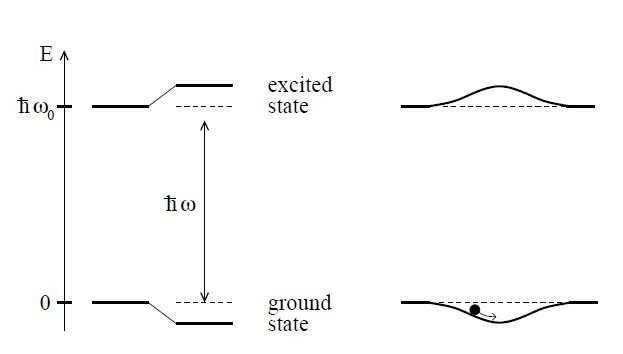
\includegraphics[width=0.5\columnwidth]{Figures/acstark.JPG} 
	\caption{\textit{Light shifts of a two-level atom. Left-hand side,
		red-detuned light ($\Delta < 0$) shifts the ground state down and the
		excited state up by same amounts. Right-hand side, a spatially
		inhomogeneous field like a Gaussian laser beam produces a
		ground-state potential well, in which an atom can be trapped. Figure and 		caption are adopted from \cite{grimm}.}}
	\label{fig:ac_stark} 
\end{figure}
Since the sign is reversed for the excited state, it is important that the atom remains in the ground state. Thus, one has to minimize the scattering with the optical potential. The scattering rate is given as \cite{grimm}
\begin{equation}
	\Gamma_{sc} = \frac{3 \pi c^2}{2 \hbar \omega_{0}^3} \left( \frac{\Gamma}{\Delta} \right) ^2 I \; .
\end{equation}
As the detuning becomes small, the laser becomes resonant with the atom causing a large increase in scattered photons. Therefore, one has to choose a large detuning in order for the potential to remain conservative. However, this comes at the cost of a weaker potential. To compensate this, a high laser intensity must be used, in order for the potential to reach sufficient depth. In practise there will be a limit to the laser power available, however, for most alkali-metal atoms the detuning is typically chosen to be large compared to the excited-state hyperfine structure splitting, which provides enough depth while being sufficient to suppress scattering events \cite{manybodyBloch}. 


\subsection{Optical Lattices}

The dipole potential in equation \eqref{eq:dipolepot} scales with the intensity of the laser. Thus, superimposing laser beams allows for creating a multitude of different potentials through the interference patterns of the lasers. A simple standing wave from two counter-propagating light fields will lead to an array of potential wells
\begin{equation}
	V(z) = - V_0 \cos^2{k z } \; ,
	\label{eq:standwave}
\end{equation}
 where $V_0 = | \frac{3 \pi c^2}{2 \omega_{0}^3} \frac{\Gamma}{\Delta} 4 I_0 |$ from equation \eqref{eq:dipolepot}. In practise, a one dimensional lattice like that of equation \eqref{eq:standwave} is created by shining a single laser beam at a mirror, whereby it interferes with itself.
\begin{figure}[!h]
	\centering
	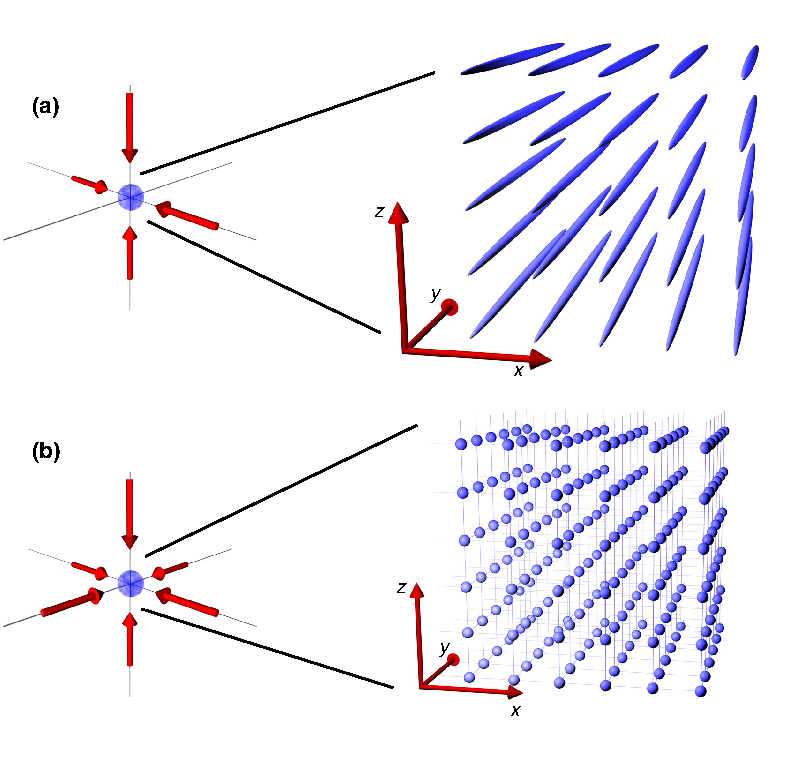
\includegraphics[width=0.7\columnwidth]{Figures/OpticalLattice.pdf} 
	\caption{\textit{\textbf{(a)} Two dimensional optical lattice formed by two mutually orthogonal laser beams. These tubes have a characteristic cigar shape, due to the Gaussian profile of the lasers. \textbf{(b)} Upon using three orthogonal laser beams, the result is a three dimensional lattice reminiscent of a cubic crystal. Figure is adopted from \cite{WideraThesis}.}}
	\label{fig:OpticalLattice} 
\end{figure}
Adding another laser beam in a different direction creates a periodic two dimensional potential. For orthogonal polarization of the two lasers, the resulting potential is purely the sum of the sinusoidal standing wave potential, as no interference term is present \cite{lewenstein}. Note, that the lattice is only well defined for distances much smaller than the waist of the laser beams, as the lattice is only present within the overlap of the two beams. Various shapes of the lattice can be achieved by adjusting the angle between the beams, however, the most common setup is using two orthogonal beam creating a square lattice of one dimensional tubes, as seen in figure \ref{fig:OpticalLattice}.
In order to create a three dimensional lattice, as seen in figure \ref{fig:OpticalLattice}, an additional third perpendicular laser beam is needed. In the center of the trap, the lattice potential is then given by
\begin{equation}
	V(x,y,z) = - V_0 \left( \cos^2{k x } + \cos^2{k y } + \cos^2{k z } \right) \; , \label{eq:3Dlattice}
\end{equation}
for distances much smaller than the beam waist. In addition to the lattice, an external harmonic confinement will be present due to the Gaussian profile of the laser beams \cite{manybodyBloch}.

\subsection{Band Structure}
Consider a periodic potential as described by equation \eqref{eq:standwave}. \textit{Bloch's Theorem} states that energy eigenstates of a periodic potential with lattice vector $\boldsymbol{R}$ and quasi-momentum $q$ can be written as Bloch waves, which takes the form
\begin{equation}
	\phi_{\boldsymbol{q}}^{(n)}(\boldsymbol{r}) = e^{i \boldsymbol{q} \boldsymbol{r}} u^{(n)}(\boldsymbol{r}) \; ,
\end{equation}
which is a plane wave modulated by a function with the same periodicity as the potential $u^{(n)}(\boldsymbol{r}) = u^{(n)}(\boldsymbol{r} + \boldsymbol{R})$. Furthermore, the Bloch waves are periodic in reciprocal space, such that $\psi_{\boldsymbol{q}}^{(n)}(\boldsymbol{r}) = \phi_{\boldsymbol{q} + \boldsymbol{G}}^{(n)}(\boldsymbol{r})$, where $\boldsymbol{G}$ is a reciprocal lattice vector. \cite{kittel} \\
This leads to an energy spectrum in the shape of bands with the periodicity of the first \textit{Brillouin Zone}. Bands are denoted by the band index $n$, and their shape is determined by both the shape and the depth of the potential. The potential depth is often denoted in units of the recoil energy $E_r = \frac{\hbar ^2 k^2}{2 m}$, where $m$ is the mass of the atom, and $k$ is the photon wave number of the light forming the optical lattice. For $V_0 = 0$, the particles are free, hence the bands will be parabolic. Meanwhile, for $V_0 \rightarrow \infty$, no interaction between different wells of the lattice can take place, as the wavefunctions of the trapped atoms will be confined to their respective well. Thus, the lattice is reduced to an array of independent harmonic oscillators, whereby the bands will appear flat with equal spacing \cite{greiner}. 

\subsection{Localized States}
For lattice potential depths within $5 E_r \leq V_0 \leq 8 E_r$, the lattice is in the \textit{tight binding limit}. Within this range, the wavefunctions of the trapped atoms will only overlap with other wells in their closest proximity. Thus, interactions between wells are almost purely of nearest neighbour nature. Due to how well localized the wavefunctions are, a basis of Wannier functions is ideal for describing the system. Wannier functions are related to Bloch functions through the Fourier transform \cite{kittel1963}
\begin{equation}
	w^{(n)}(\boldsymbol{r}) = \frac{1}{\sqrt{N_L}} \sum_{q} e^{ -i \boldsymbol{q} \boldsymbol{R} } \phi_{\boldsymbol{q}}^{(n)}(\boldsymbol{r}) \; ,
\end{equation} 
where $N_L$ is the number of primitive cells of the lattice. The Wannier functions are well localized and centred around the lattice at site $\boldsymbol{R}$. In the case of a separable periodic potential, like that of equation \eqref{eq:3Dlattice}, the single-particle problem becomes dimensional \cite{kohn1959analyticWannier}. Lastly, Wannier functions obey the orthonormality relation
\begin{equation}
	\int \mathrm{d^3}r \; \; w^{(n) *}(\boldsymbol{r} - \boldsymbol{R}) w^{(n')}(\boldsymbol{r} - \boldsymbol{R'}) = \delta_{n,n'} \delta_{\boldsymbol{R},\boldsymbol{R}'} \; ,
\end{equation}
thus forming a complete basis \cite{manybodyBloch}. 
\begin{figure}[!h]
	\centering
	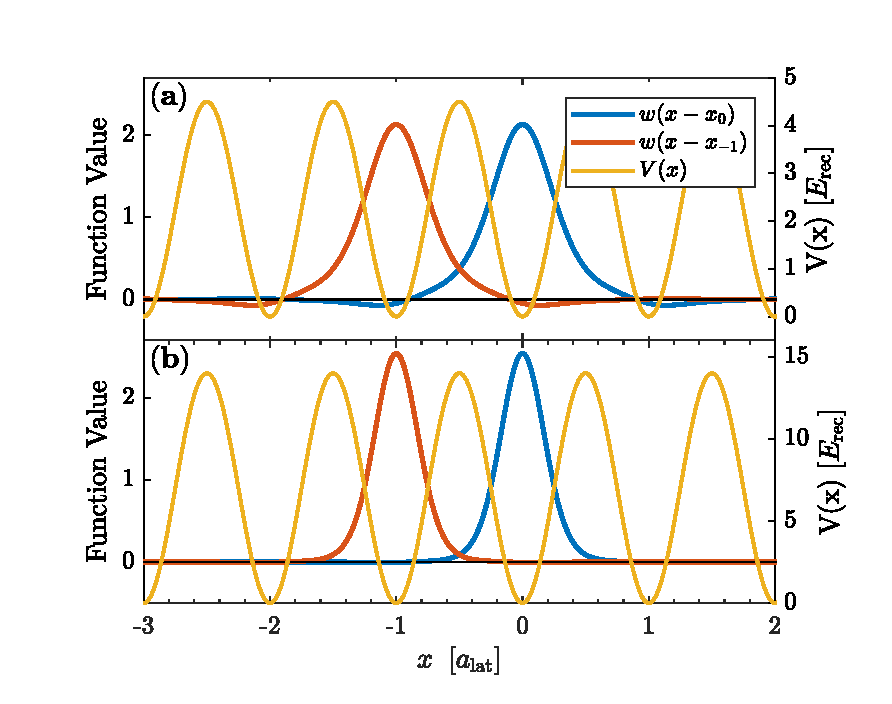
\includegraphics[width=0.8\columnwidth]{Figures/WannierFunctions.pdf} 
	\caption{\textit{Two one-dimensional Wannier functions plotted for lattice depths of $V_0 = 4.5 E_r$ \textbf{(a)} and $V_0 = 14 E_r$ \textbf{(b)} respectively.}}
	\label{fig:WannierPlot} 
\end{figure}
Figure \ref{fig:WannierPlot}.a shows Wannier functions plotted for lattice potential depths within the tight binding limit. As evident from the plot, the functions overlap with only their nearest neighbours. In the case of a more shallow lattice, the functions would extends to further wells, while they will tend towards a Gaussian shape as the lattice depth increases \cite{greiner}, which can be seen in figure \ref{fig:WannierPlot}.b.



\section{Bose-Einstein Condensates}

Bosons are particles of integer spin, whose statistics obey those of a Bose-Einstein distribution
\begin{equation}
	n_i = \frac{g_i}{\exp \left( \left( \varepsilon_i -\mu \right) / k_B T \right) - 1} \; , \label{eq:BHdistribution}
\end{equation} 
where $i$ denotes the state, $n_i$ is the population of the state, $g_i$ is its degeneracy, $\varepsilon_i$ is its energy, $\mu$ is the chemical potential, $k_B$ is the Boltzmann constant, and $T$ is the temperature. One important feature of bosons is that, unlike fermions, multiple particles can occupy the same quantum state. At higher temperatures the energy spectrum is practically continues, whereby this property has little effect, as two particles occupying the same single-particle state is highly unlikely. However, at low temperatures the energy spectrum systems often become increasingly discrete, hence the statistics of the particles becomes very important. As evident from equation \eqref{eq:BHdistribution}, the population of the ground state diverges as $T \to 0$. However, even below the finite temperature, $T_c$, one will observe a macroscopic population of the ground state. $T_c$ is called the critical temperature, and marks the point where multiple particles will start forming a Bose-Einstein Condensate (BEC). \cite{pethick2002bose}

\subsection{Non-Interacting Particles}
In the case of non-interacting particles and zero temperature, all particles of a Bose gas can be described by identical single-particles wavefunctions $\phi (\boldsymbol{r}_i)$. Hence, the many-body wavefunction is simply given by the product 
\begin{equation}
	\Psi (\boldsymbol{r}_1 , \ldots , \boldsymbol{r}_N) = \prod_{i}^{N} \phi (\boldsymbol{r}_i) \; .
\end{equation}
Such a product state can be described by a single macroscopic wavefunction
\begin{equation}
	\psi (\boldsymbol{r}) = \sqrt{N} \varphi (\boldsymbol{r}) \; , \label{eq:psi_NIBEC}
\end{equation}
where $\phi (\boldsymbol{r})$ is the wave function of the single-particle state, in which the bosons condensate into \cite{PenroseOnsager}.

\subsubsection{Second-Quantization}
When describing Bose-Einstein condensates it is very convenient to work in second quantization, which describes the number of particle in each state rather than the state of each particle.\\
First, consider a basis of single particle states $\{ \ket{n} \}$, namely a Fock basis. In this space particles are created or annihilated through their respective operators
\begin{equation}
	\hat{a}_{\mu}^{\dag} \ket{0_\mu} = \ket{1_\mu} \; .
\end{equation}
For bosons the creation and annihilation operators fulfill the commutation relations
\begin{equation}
[\hat{a}_\nu,\hat{a}_\mu]=[\hat{a}_\nu^\dagger,\hat{a}_\mu^\dagger]=0 \quad , \quad [\hat{a}_\nu,\hat{a}_\mu^\dagger]=\delta_{\nu,\mu} \; , 
\end{equation}
with the number operator given as
\begin{equation}
	\hat{n}_{\mu} = \hat{a}_{\mu}^{\dag} \hat{a}_{\mu} \; .
\end{equation}
In second quantization many-body states are described by the occupation of the individual Fock states. Thus, a creation operator will raise the number of particles in its corresponding state by one, while the annihilation operator will lower it:
\begin{align}
\hat{a}^\dagger \ket{N_0,N_1, \ldots , N_{\nu},\ldots}&= \sqrt{N_\nu+1}\ket{N_0,N_1, \ldots , N_{\nu}+1,\ldots} \\
\hat{a} \ket{N_0,N_1, \ldots , N_{\nu},\ldots}&= \sqrt{N_\nu}\ket{N_0,N_1, \ldots , N_{\nu}-1,\ldots} .
\end{align}
Likewise, the number operator $\hat{n}_{\mu}$ will count the number of particles in its corresponding state.\\
These operators can be combined with an orthonormal basis of spatial wavefunctions $\{ \phi_k \}$ in order to create field operators
\begin{equation}
	\hat{\psi}(\boldsymbol{r}) = \; \sum_{k} \phi_k \hat{a}_{k} \quad , \quad \hat{\psi}^{\dag}(\boldsymbol{r}) = \; \sum_{k} \phi_{k}^{*} \hat{a}_{k}^{\dag} \; ,
\end{equation}
where $\hat{\psi}(\boldsymbol{r})$ will create a particle at location $\boldsymbol{r}$. For bosons the field operators fulfil the commutation relations \cite{bruus}
\begin{equation}
	\left[ \hat{\psi}(\boldsymbol{r}) \; , \; \hat{\psi}^{\dag}(\boldsymbol{r'}) \right] = \; \delta(\boldsymbol{r} - \boldsymbol{r}') \quad , \quad
	\left[ \hat{\psi}(\boldsymbol{r}) \; , \; \hat{\psi}(\boldsymbol{r'}) \right] = \; 0 \; .
\end{equation}
Now, consider a gas of non-interacting bosons described by equation \eqref{eq:psi_NIBEC}, where $\epsilon_k$ is the energy of the $k$'th single-particle state. Due to the completeness of the basis of single-particle wavefunctions, $\{ \phi_k \}$, the creation operator can be expressed as
\begin{equation}
	\hat{a}_k = \int \mathrm{d^3} r \;  \phi_{k}^*(\boldsymbol{r}) \hat{\psi}(\boldsymbol{r}) \; .
\end{equation}
Using this, the Hamiltonian can be written as
\begin{align}
	\hat{H}^{(0)} =& \; \sum_{k} \epsilon_k \hat{a}_{k}^{\dag} \hat{a}_{k} \nonumber \\
		=& \;  \sum_{k} \int \mathrm{d^3}r_1 \mathrm{d^3}r_2 \; \epsilon_k \phi_k (\boldsymbol{r_1}) \phi_{k}^* (\boldsymbol{r_2})\; \; \hat{\psi}^{\dag} (\boldsymbol{r_1}) \hat{\psi} (\boldsymbol{r_2}) \nonumber \\
		=& \; \int \mathrm{d^3}r  \; \hat{\psi}^{\dag}(\boldsymbol{r}) \left( - \frac{\hbar^2}{2 m} \nabla^2 + U(\boldsymbol{r})\right) \hat{\psi}(\boldsymbol{r})
		\label{hamil2nd}
\end{align}

\subsection{Weakly Interacting Particles}
A characteristic of a BEC is its low temperature and density. Thus, is it a valid approximation to only consider two-particle interactions
\begin{equation}
	\hat{H}^{(2)} = \frac{1}{2} \sum_{i \neq j} V(\boldsymbol{r_i} - \boldsymbol{r_j}) \; .
\end{equation}
At low energies all interactions can be considered of s-wave nature, because
all waves of higher angular momentum are reflected by the centrifugal barrier. Furthermore, for cold gases the thermal de Broglie wavelength is much larger than the effective extension of the interaction potential. Therefore, the actual shape of the scattering potential is irrelevant, hence one can replace it with a pseudo-potential
\begin{equation}
	V(\boldsymbol{r} - \boldsymbol{r'}) = g \; \delta(\boldsymbol{r} - \boldsymbol{r'}) = \frac{4 \pi \hbar^2 a}{m} \delta(\boldsymbol{r} - \boldsymbol{r'}) \; ,
\end{equation}
which results in the same scattering phase as the real, more complicated scattering potential. Thus, the interaction of cold atoms is fully determined by the scattering length, $a$ \cite{greiner}.\\
Introducing the density operator
\begin{equation}
	\hat{\rho}(\boldsymbol{r}) = \hat{\psi}^{\dag}(\boldsymbol{r}) \hat{\psi}(\boldsymbol{r}) \; ,
\end{equation}
allows writing $\hat{H}^{(2)}$ in second quantization
\begin{align}
	\hat{H}^{(2)} &= \frac{1}{2} \int \mathrm{d^3}r_1 \mathrm{d^3}r_2 V(\boldsymbol{r_1} - \boldsymbol{r_2}) \hat{\psi}^{\dag}(\boldsymbol{r_1}) \hat{\psi}(\boldsymbol{r_1}) \left( \hat{\psi}^{\dag}(\boldsymbol{r_2}) \hat{\psi}(\boldsymbol{r_2}) - \delta(\boldsymbol{r_1} - \boldsymbol{r_2}) \right) \\
	&= \frac{1}{2} \int \mathrm{d^3}r_1 \mathrm{d^3}r_2  \hat{\psi}^{\dag}(\boldsymbol{r_1}) \hat{\psi}^{\dag}(\boldsymbol{r_2}) V(\boldsymbol{r_1} - \boldsymbol{r_2}) \hat{\psi}(\boldsymbol{r_1}) \hat{\psi}(\boldsymbol{r_2}) \; .
\end{align}
Combining this with the basic Hamiltonian of equation \eqref{hamil2nd}, gives the full Hamiltonian in second quantization
\begin{align}
	\hat{H} &= \hat{H}^{(0)} + \hat{H}^{(2)} \\
	& = \int \mathrm{d^3}r \ \hat{\psi}^{\dag}(\boldsymbol{r}) \left( - \frac{\hbar^2}{2 m} \nabla^2 + U(\boldsymbol{r})\right) \hat{\psi}(\boldsymbol{r}) + \frac{1}{2} \int \mathrm{d^3}r_1 \mathrm{d^3}r_2  \ \hat{\psi}^{\dag}(\boldsymbol{r_1}) \hat{\psi}^{\dag}(\boldsymbol{r_2}) V(\boldsymbol{r_1} - \boldsymbol{r_2}) \hat{\psi}(\boldsymbol{r_1}) \hat{\psi}(\boldsymbol{r_2})
	\label{hamilint}
\end{align}
Using this Hamiltonian to try and solve the Heisenberg equations of motion for the field operators leads to
\begin{equation}
	i \hbar \frac{\partial }{\partial t} \hat{\psi}(\boldsymbol{r}) = \left[ \hat{\psi}(\boldsymbol{r}) \; , \; \hat{H}  \right] = \left( - \frac{\hbar^2}{2 m} \nabla^2 + U(\boldsymbol{r}) + g \hat{\psi}^{\dag}(\boldsymbol{r}) \hat{\psi}(\boldsymbol{r}) \right) \hat{\psi}(\boldsymbol{r}) \; ,
\end{equation}
which is not solvable in general. However, in the scenario of a BEC the scattering length $a$ is much less than the mean inter-particle distance, such that $n a^3 \ll 1$, where $n$ is the density of the gas. In this regime the mean-field approximation is viable
\begin{equation}
	\hat{\psi}(\boldsymbol{r}) = \psi(\boldsymbol{r}) + \delta \hat{\psi}(\boldsymbol{r}) \; ,
\end{equation}
where $\psi(\boldsymbol{r})$ is the mean-field given by equation \eqref{eq:psi_NIBEC}, and $\delta \hat{\psi}(\boldsymbol{r})$ is fluctuations from the mean. If $\braket{\delta \hat{\psi}(\boldsymbol{r})} = 0$, the fluctuations can be neglected, leading to the Gross-Pitaevskii equation \cite{Gross1961,Pitaevskii}
\begin{equation}
	i \hbar \frac{\partial }{\partial t} \hat{\psi}(\boldsymbol{r}) = \left( - \frac{\hbar^2}{2 m} \nabla^2 + U(\boldsymbol{r}) + g |\psi(\boldsymbol{r})|^2 \right) \psi(\boldsymbol{r}) \; .
\end{equation}
The Gross-Pitaevskii equation is very similar to the Schrödinger equation with exception of the non-linear term $g |\psi(\boldsymbol{r})|^2$, which can make the equation hard to solve in regions of low density.



\section{Bose-Hubbard Model of Interacting Bosons in a Lattice} \label{sec:BHmodel}
The Bose-Hubbard model describes weakly interacting bosons in a periodic lattice within the tight binding limit. The model is perfectly capable of predicting results with good accuracy, however, two conditions must hold in order for the it to be valid: (i) both the thermal energy and the mean interaction energy at a single site must be much smaller than the separation to first excited band, $\hbar \omega_0$, and (ii) the Wannier functions decay essentially within the length of the lattice constant \cite{manybodyBloch}.\\
Under these conditions one is assured that only the lowest band is taken into account, and that only nearest-neighbour interactions take place.\\
The Bose-Hubbard model is interesting, as it supports two distinct phases: the Superfluid phase and the Mott-Insulator phase. Furthermore, the model contains effects such as a quantum phase transition between the two phases mentioned above, which can be crossed without any change in external parameters. 


\subsection{The Bose-Hubbard Hamiltonian}
Consider the Hamiltonian for bosonic particles in a trapping potential (described by equation \eqref{hamilint}) in one dimension. For a periodic lattice potential in the tight binding limit it is favourable to work in a basis of localized Wannier functions. Expanding the field operators of the Hamiltonian in equation \eqref{hamilint} in  the Wannier basis yields \cite{Jaksch}
\begin{align}
	\hat{H} &= \int \mathrm{d}x \sum_{i j} w^*(x-x_i) \hat{a}_{i}^{\dag} \left( - \frac{\hbar^2}{2 m} \nabla ^2 + V(x) \right) w(x-x_j) \hat{a}_j \nonumber \\
	& \quad + g \int \mathrm{d}x \sum_{i j k l} w^*(x-x_i) w^*(x-x_j) w(x-x_k) w(x-x_l) \hat{a}_{i}^{\dag} \hat{a}_{j}^{\dag} \hat{a}_{k} \hat{a}_{l} \\
	&= - \sum_{i j } J_{i j} \hat{a}_{i}^{\dag} \hat{a}_{j} + \sum_{i j k l} U_{i j k l} \hat{a}_{i}^{\dag} \hat{a}_{j}^{\dag} \hat{a}_{k} \hat{a}_{l} \; ,
\end{align}
where
\begin{align}
	J_{i j} &= - \int \mathrm{d}x \ w^*(x-x_i) \left( - \frac{\hbar^2}{2 m} \nabla ^2 + V(x) \right) w(x-x_j) \label{eq:BHparamJ} \\
	U_{i j k l} &= g \int \mathrm{d}x \ w^*(x-x_i) w^*(x-x_j) w(x-x_k) w(x-x_l) 
\end{align}
Since the system is periodic, one can consider a single site, $i = 0$, as representative for the entire lattice. In this way, the different terms of the Hamiltonian can be interpreted as follows:
\begin{align}
	J_{0 0} &= \text{constant energy offset} \nonumber \\
	J_{0 1} &= \text{"overlap matrix element" to neighbouring site} \nonumber \\
	J_{0 2 - 0 \infty} &= \text{"overlap matrix element" to further sites} \nonumber \\
	U_{0 0 0 0} &= \text{on-site interaction for two particles} \nonumber \\
	U_{0 i i 0} &= \text{interaction off-site} \nonumber \\
	U_{0 0 0 1} &= \text{interaction  + tunnelling , off-site} \nonumber 
\end{align}
Due to the rapid decay of the Wannier functions, the overlap of wavefunctions is limited to their nearest neighbour. Dropping all exponentially suppressed terms and constant offsets yields the Bose-Hubbard Hamiltonian
\begin{equation}
	\hat{H} = - J \sum_{\langle i,j \rangle} \hat{a}_{i}^{\dag} \hat{a}_{j} + \frac{U}{2} \sum_{i} \hat{n}_i \left( \hat{n}_i -1 \right) + \sum_{i} \varepsilon_i \hat{n}_i \; ,
	\label{BHhamil}
\end{equation}
where $J = J_{0 1}$, the bracket $\langle i,j \rangle$ denotes only counting neighbouring pairs, and
\begin{equation}
	U = U_{0 0 0 0} = g \int \mathrm{d}x \ |w(x)|^4 \; .
	\label{eq:BHparamU}
\end{equation}
The first term of the Bose-Hubbard Hamiltonian describes the kinematics within the model, which takes the form of tunneling between neighbouring sites. This is interpreted by annihilating a particle at site $j$ while creating a particle at site $i$. The second term describes the interaction between particles within a single site, and the last term $\sum_{i} \varepsilon_i \hat{n}_i$ takes into account a possible potential offset at different sites.
\begin{figure}[!h]
	\centering
	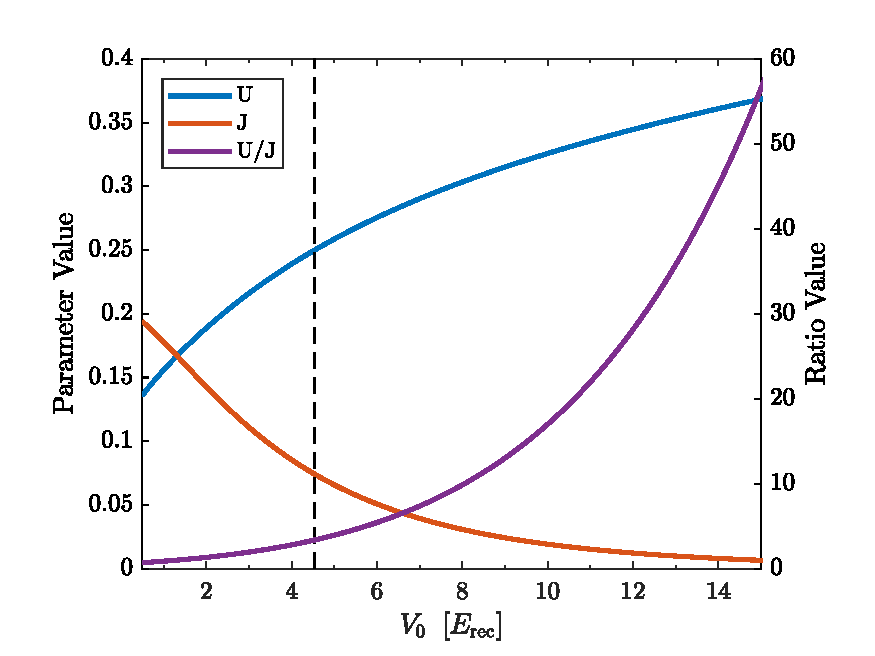
\includegraphics[width=0.7\columnwidth]{Figures/UJparameters.pdf} 
	\caption{\textit{Tunneling matrix element, $J$, of eq. \eqref{eq:BHparamJ} and interaction strength, $U$, of eq. \eqref{eq:BHparamU} as function of lattice depth. The parameters are calculated for Rubidium-87 atoms in an optical lattice with wavelength $\lambda = 1064 \mathrm{nm}$. The phase transition between the superfluid and Mott Insulator is marked with a dashed line.}}
	\label{fig:UJparameters} 
\end{figure}
Figure \ref{fig:UJparameters} illustrates the parameters of the Bose-Hubbard model as function of the lattice depth. The tunneling matrix element falls of very quickly with increasing lattice depth, as the Wannier functions become localized to their respective wells, thus reducing their overlap. The localization of the Wannier functions also causes the on-site interaction strength to increase.

\subsection{Phases of the Bose-Hubbard Model}

The Bose-Hubbard model supports two quantum phases: The \textit{Superfluid} phase and the \textit{Mott Insulator} phase. These phases depend on the ratio $J/U$, and can be described separately by examining the ground state of the Bose-Hubbard Hamiltonian in the two extreme limits of the $J/U$ ratio.

\subsubsection{Superfluid Phase}
For a system where the tunneling matrix element $J$ is dominant, the lowest energy is obtained by delocalizing the atoms over the entire lattice. Thereby the wavefunction will be a product over single-particle states, and the system will be a superfluid \cite{greiner}.\\
Consider the case of negligible interactions and a lattice of equal depth. In this scenario the Bose-Hubbard Hamiltonian reduces to
\begin{equation}
	\hat{H} = \hat{H}_J = - J \sum_{\langle i,j \rangle} \hat{a}_{i}^{\dag} \hat{a}_{j} \; , 
	\label{hamilSF}
\end{equation}
which is completely periodic within the lattice due to the lack of site specific terms. This leads to solutions in the shape of Bloch waves. The Fourier transform of the annihilation and creation operators
\begin{equation}
	\hat{a}_j = \frac{1}{N_L} \sum_{q}  e^{i q x_j} \hat{a}_q \quad , \quad
	\hat{a}_{j}^{\dag} = \frac{1}{N_L} \sum_{q}  e^{-i q x_j} \hat{a}_{q}^{\dag}
\end{equation}
allows for writing the Hamiltonian \eqref{hamilSF} in momentum space
\begin{equation}
	\hat{H}_J = - J \sum_{q = - \infty}^{\infty} \left( e^{- i q d } + e^{i k d} \right) \hat{n}_q \; ,
\end{equation}
where $d$ is the lattice distance. In momentum space the Hamiltonian is diagonal and results in a continuous energy spectrum
\begin{equation}
	E_q = -2 J \cos(q d) \; .
	\label{SFenergy}
\end{equation}
Thus, the excitation spectrum of the Superfluid is said to be gapless.

The lowest energy is of the system is obtained for $q = 0$, whereby the ground state is
\begin{equation}
	\ket{\Psi_{SF}} =  \frac{1}{\sqrt{N!}} \left( \hat{a}_{q = 0}^{\dag} \right) ^N \ket{0} = \frac{1}{\sqrt{N!}} \left( \frac{1}{N_L} \sum_{j = 1}^{N_L} \hat{a}_{j}^{\dag} \right) ^N \ket{0} \; ,
\end{equation} 
where $N$ is the number of particles. This state supports a well defined macroscopic phase on each lattice site, since the many-body state is a product over identical single-particle states \cite{greiner}. With all particle condensed into the $q = 0$ momentum space state, the particles are completely de-localized in real space, which can be seen by taking the Fourier transform. For large $N,N_L \rightarrow \infty$ at fixed density $N/N_L$ the state becomes indistinguishable from having coherent states, $\ket{\alpha} $, on all lattice sites \cite{manybodyBloch}
\begin{equation}
	\ket{\Psi_{SF}} \approx \prod_j \left( e^{\sqrt{N/N_L} \hat{a}_{j}^{\dag}} \right) \ket{0} = \ket{\alpha_1} \otimes \ket{\alpha_2} \otimes \ldots
	\label{stateSF}
\end{equation}
\begin{figure}[!h]
	\centering
	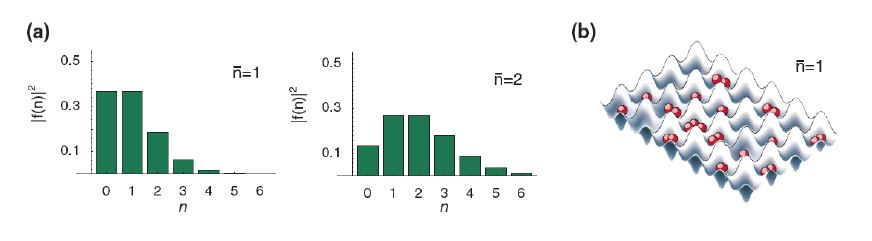
\includegraphics[width=0.8\columnwidth]{Figures/f(n)_SF.JPG} 
	\caption{\textbf{(a)}The statistics for the number of particles per lattice site $n$ for a filling fraction of $\bar{n}=1$ and $\bar{n}=2$ in the superfluid phase. \textbf{(b)} Illustration of the particles in the lattice. There will be large fluctuations of the number of particles found at each lattice site at a given time. Figure and caption adopted from \cite{greiner}.}
	\label{fig:f(n)_SF} 
\end{figure}
Since bosonic operators at different sites commute, the superfluid state can be factorized into a product of local coherent states.
Coherent states are eigenstates of the annihilation operator $\hat{a} \ket{\alpha} = \alpha \ket{\alpha}$, where $|\alpha |^2$ can be considered the particle density of the system, and $\alpha = |\alpha| e^{i \phi}$, with $\phi$ being a global phase. Utilizing the coherent state form of the wavefunction (eq. \eqref{stateSF}) the average filling fraction $\bar{n}$ can be calculated
\begin{equation}
	\bar{n} = \braket{\hat{n}_i} = \bra{\Psi_{SF}} \hat{a}_{j}^{\dag} \hat{a}_{j} \ket{\Psi_{SF}} = \frac{N}{N_L} \; ,
\end{equation}
as well as the fluctuations of particle number per site
\begin{equation}
	\frac{\sqrt{\Delta \bar{n}^2}}{\bar{n}} \sim \frac{1}{\sqrt{\bar{n}}} \; .
\end{equation}
Therefore, the probability distribution for the number of atoms at a given site is Poissonian, which can be seen in figure \ref{fig:f(n)_SF}. Due to the relatively large fluctuation of particle number per site, one would find a somewhat random number of atoms at a given site in a measurement. In the presence of a finite interaction, $U$, the resulting distribution would be sub Poissonian due to number squeezing \cite{greiner}.


\subsubsection{Mott-Insulator Phase}
In the case of negligible tunneling, only the on-site interaction between the atoms has to be taken into account, and the Bose-Hubbard Hamiltonian reduces to
\begin{equation}
	\hat{H} = \hat{H}_U = \frac{U}{2} \sum_{i} \hat{n}_i \left( \hat{n}_i -1 \right) \; ,
	\label{hamilMott}
\end{equation}
which is quadratic in $\hat{n}_i$. This heavily penalizes having multiple particles at the same site. Thus, the ground state of the system will be an equal distribution of all the particles throughout the lattice. Any fluctuations from this average will increase the energy, whereby the phase is said to be incompressible \cite{Gemelke2009}. This incompressibility can be formulated as $\frac{\partial n}{\partial \mu} = 0$, where $\mu$ is the chemical potential, and is the defining property of the Mott-Insulator \cite{manybodyBloch}.\\
\begin{figure}[!h]
\centering
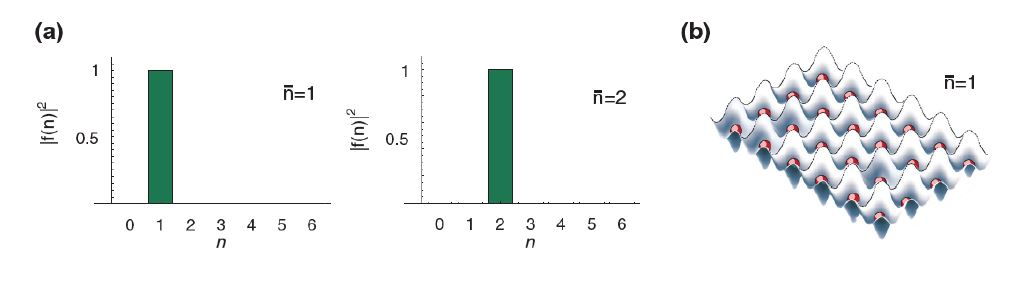
\includegraphics[width=0.8\columnwidth]{Figures/f(n)_M.JPG} 
\caption{\textbf{(a)}The statistics for the number of particles per lattice site $n$ in the Mott-insulator phase, for a filling fraction of $\bar{n}=1$ and $\bar{n}=2$. \textbf{(b)} Illustration of the particles in the lattice. The particles does not hop around in the lattice and are equally distributed. Caption and figure are adapted from \cite{greiner}.}
\label{fig:f(n)_M} 
\end{figure}
Consider the case $\bar{n} = 1$, (average filling of one particle per site). This can be described by a state with a single particle located on each site \cite{manybodyBloch}
\begin{equation}
	\ket{\Psi_{Mott}} = \prod_j \hat{a}_{j}^{\dag} \ket{0} \; .
	\label{eq:MIstate}
\end{equation}
This is a simple product of local Fock states with precisely
one atom per site, which is illustrated in figure \ref{fig:f(n)_M}. This is the configuration of atoms, which minimizes the energy with regards to the Hamiltonian of eq. \eqref{hamilMott}. Any fluctuation from unit occupancy will increase the energy, as merely a single double occupancy will increase the energy by $U$. Thereby, unlike the energy spectrum of the Superfluid, the Mott-Insulator spectrum is gapped. As long as the gain in kinetic energy due to hopping, $J$, is smaller than the on-site interaction, $U$, the atoms remain localized. However, for $J > 0$ the ground state is no longer a the simple product state described in eq. \eqref{eq:MIstate} \cite{manybodyBloch}. As $J$ increases, the gap in the excitation spectrum will gradually decrease until the transition to the superfluid is reached and the spectrum becomes gapless.\\
While the Mott-Insulator phase has complete localization, the phases on the individual sites have obtained maximum uncertainty. Therefore, no phase coherence between different sites is present \cite{greiner}.


\subsection{Quantum Phase Transition}
Consider once again the full Bose-Hubbard Hamiltonian \eqref{BHhamil}. The superfluid and the Mott-Insulator account for the two limits of the ratio $J/U$, however, it order to understand the full phase diagram of the Bose-Hubbard model one has to derive the $U_{crit}$ for which the phase transition occurs. There are several ways of doing this - one of them is looking at a mean-field solution of the Bose-Hubbard model. For simplicity the scenario $T=0$ is treated here. Even without a change of temperature the phase transition still happens, hence the label \textit{quantum phase transition} referring to the fact that the phase transition can happen without change of external parameters \cite{Sachdev2007QPT}.\\
Applying the mean field approximation to the annihilation operator yields
\begin{equation}
	\hat{a}_j = \psi + \delta \hat{a}_j \; ,
\end{equation}
where $\psi$ is the locally constant mean field, and $\delta \hat{a}_j$ is the fluctuation term. Inserting this into the Hamiltonian yields
\begin{equation}
	\hat{H}_{MF} = -J \sum_{\langle i,j \rangle} \left( \psi^* + \delta \hat{a}_{i}^{\dag} \right) \left( \psi + \delta \hat{a}_{j} \right) + \text{int.}
\end{equation}
Instead of considering the Hamiltonian as a whole, it can be considered as a sum of local on-site Hamiltonians
\begin{equation}
	\hat{H}_{MF} = \sum_{i} \hat{h}_i \; .
\end{equation}
For a homogeneous system $\hat{h}_i = \hat{h}_j \; \; \forall i,j$. One can write the kinetic part of the Hamiltonian locally if one assumes small fluctuations from the mean field
\begin{align}
  \hat{a}_{i}^{\dag} \hat{a}_{j} &= \left( \psi^* + \delta \hat{a}_{i}^{\dag} \right) \left( \psi + \delta \hat{a}_{j} \right) \nonumber \\
  &= \psi^* \psi + \psi^* \delta \hat{a}_j + \psi \delta \hat{a}_{i}^{\dag} + \delta \hat{a}_{i}^{\dag} \delta \hat{a}_{j} \nonumber \\
  & \approx \psi^* \psi + \psi^* \left( \hat{a}_j - \psi \right) + \psi \left( \hat{a}_{i}^{\dag} - \psi^* \right) \nonumber \\
&= \psi^* \hat{a}_j + \psi \hat{a}_{i}^{\dag} - \psi^* \psi
\end{align}
Since every term only contains a single index, one can let $j \rightarrow i$ leaving a local description
\begin{equation}
	\hat{h}_i = J z \psi^* \psi - J z \left( \psi^* \hat{a}_i + \psi \hat{a}_{i}^{\dag} \right) + \frac{U}{2} \hat{n}_i \left( \hat{n}_i -1 \right) + \mu_i \hat{n}_i \; ,
	\label{localhamil}
\end{equation}
where $z$ is the number of neighbours of site $i$ \cite{vanoosten}. The last term added is a chemical potential, which is needed due to the lack of a fixed particle number locally prompting the use of a Grand Canonical Ensemble description.\\
Landau theory is a general theory regarding phase transitions, which states that in the vicinity of a critical point, one may expand the free energy in a power series of some order parameter $m$. Thus, in order to find $U_{crit}$, equation \eqref{localhamil} must be minimized. In this case this order parameter is the mean field, hence
\begin{equation}
	E_{MF} = \text{const. } + a |\psi|^2 + b |\psi|^4 + \ldots \label{eq:landau}
\end{equation} 
Plotting this yields an effective potential, which dictates certain properties of the system.
The potential is symmetric in the complex plane allowing the system to have any phase. Furthermore, at some critical value of $a$, (here $a = 0$), the potential will shift from having a single central minimum to having minima at some $|\psi|$. This is a U(1) spontaneous symmetry breaking, which in Landau theory is associated with a phase transition \cite{plischke}. Thus, one need to compute the parameter $a$ of equation \eqref{eq:landau}.\\
One method is using second order perturbation theory, where the $\hat{\psi} = 0$ case is solved exactly, followed by adding a small $\hat{\psi}$ as a perturbation
\begin{equation}
	\hat{h}_{i}^{(0)} = J z \left( \psi^* \psi \right) + \frac{U}{2} \hat{n}_i \left( \hat{n}_i -1 \right) - \mu \hat{n}_i \; .
\end{equation} 
Since the zero-order solution only contain number operators, the ground state of the solution can be expressed in the Fock basis:
\begin{align*}
	\ket{0} \quad &\text{for} \quad \mu < 0 \\
	\ket{1} \quad &\text{for} \quad 0 \leq \mu < U \\
	\ket{2} \quad &\text{for} \quad U \leq \mu < 2 U \\
	& \vdots
\end{align*} 
Adding on the first order perturbation to the energy
\begin{equation}
	E_{i}^{(1)} = \bra{n} \delta \hat{a}_i \ket{n} = 0 \; ,
\end{equation}
yields nothing, thus requiring the use of a second order perturbation
\begin{equation}
	E_{i}^{(2)} = \sum_{n \neq g} \frac{|\bra{n} \delta \hat{h}_i \ket{g}|^2}{E_{g}^{(0)} - E_{n}^{(0)}} \; .
\end{equation}
Here the perturbation Hamiltonian
\begin{equation}
	\hat{h}_i = - z J \left( \hat{a}_i \psi^* + \psi \hat{a}_{i}^{\dag} \right)
\end{equation}
contains only single creation/annihilation operators, whereby
\begin{equation}
	\bra{n} \delta \hat{h}_i \ket{g} = 0 \quad \text{for} \quad |n - g| \neq 1 \; .
\end{equation}
Hence, for each annihilation and creation operator only two matrix elements will give a contribution
\begin{align*}
	\bra{n}  \hat{a}_{i}^{\dag} \ket{n-1} &= \sqrt{n} \braket{n|n} \\
	\bra{n+1}  \hat{a}_{i}^{\dag} \ket{n} &= \sqrt{n+1} \braket{n|n} \\
	& \vdots
\end{align*}
With this the second order perturbation energy reduces to
\begin{align}
	E_{i}^{(2)} &= \left( J z \right)^2 |\psi|^2 \left( \frac{n}{E_{g}^{(0)}- E_{n-1}^{(0)}} +  \frac{n+1}{E_{n}^{(0)}- E_{n+1}^{(0)}} \right) \nonumber \\
	&= \left( J z \right)^2 |\psi|^2 \left( \frac{n}{U(n-1) - \mu} + \frac{n+1}{\mu - U n} \right) \; .
\end{align}
Since $a$ is the pre-factor of all terms proportional $|\psi|^2$, collecting those across from all the perturbations yields the approximation 
\begin{equation}
	a = J z + \left( J z \right)^2 |\psi|^2 \left( \frac{n}{U(n-1) - \mu} + \frac{n+1}{\mu - U n} \right) \; .
\end{equation} 
As stated earlier $U_{crit}$ can be found from $a = 0$:
\begin{equation}
	0 \overset{!}{=} 1 + \frac{n}{\bar{U} (n-1) - \bar{\mu}} + \frac{n+1}{\bar{\mu} - \bar{U} n} \; ,
\end{equation}
with $\bar{\mu} = \frac{\mu}{J z}$ and $\bar{U} = \frac{U}{J z}$. Finally, the solution for the chemical potential is \cite{vanoosten}
\begin{equation}
	\bar{\mu}_{\pm} = \frac{1}{2} \left( \bar{U}(2n -1) \pm \frac{1}{2} \sqrt{\bar{U}^2 - 2 \bar{U} (2 n +1)} \right) \; .
\end{equation}
Understanding this result can be done be examining figure \ref{fig:SFMOTT}, which displays a phase diagram of the Bose-Hubbard model.  
\begin{figure}[h]
	\centering
	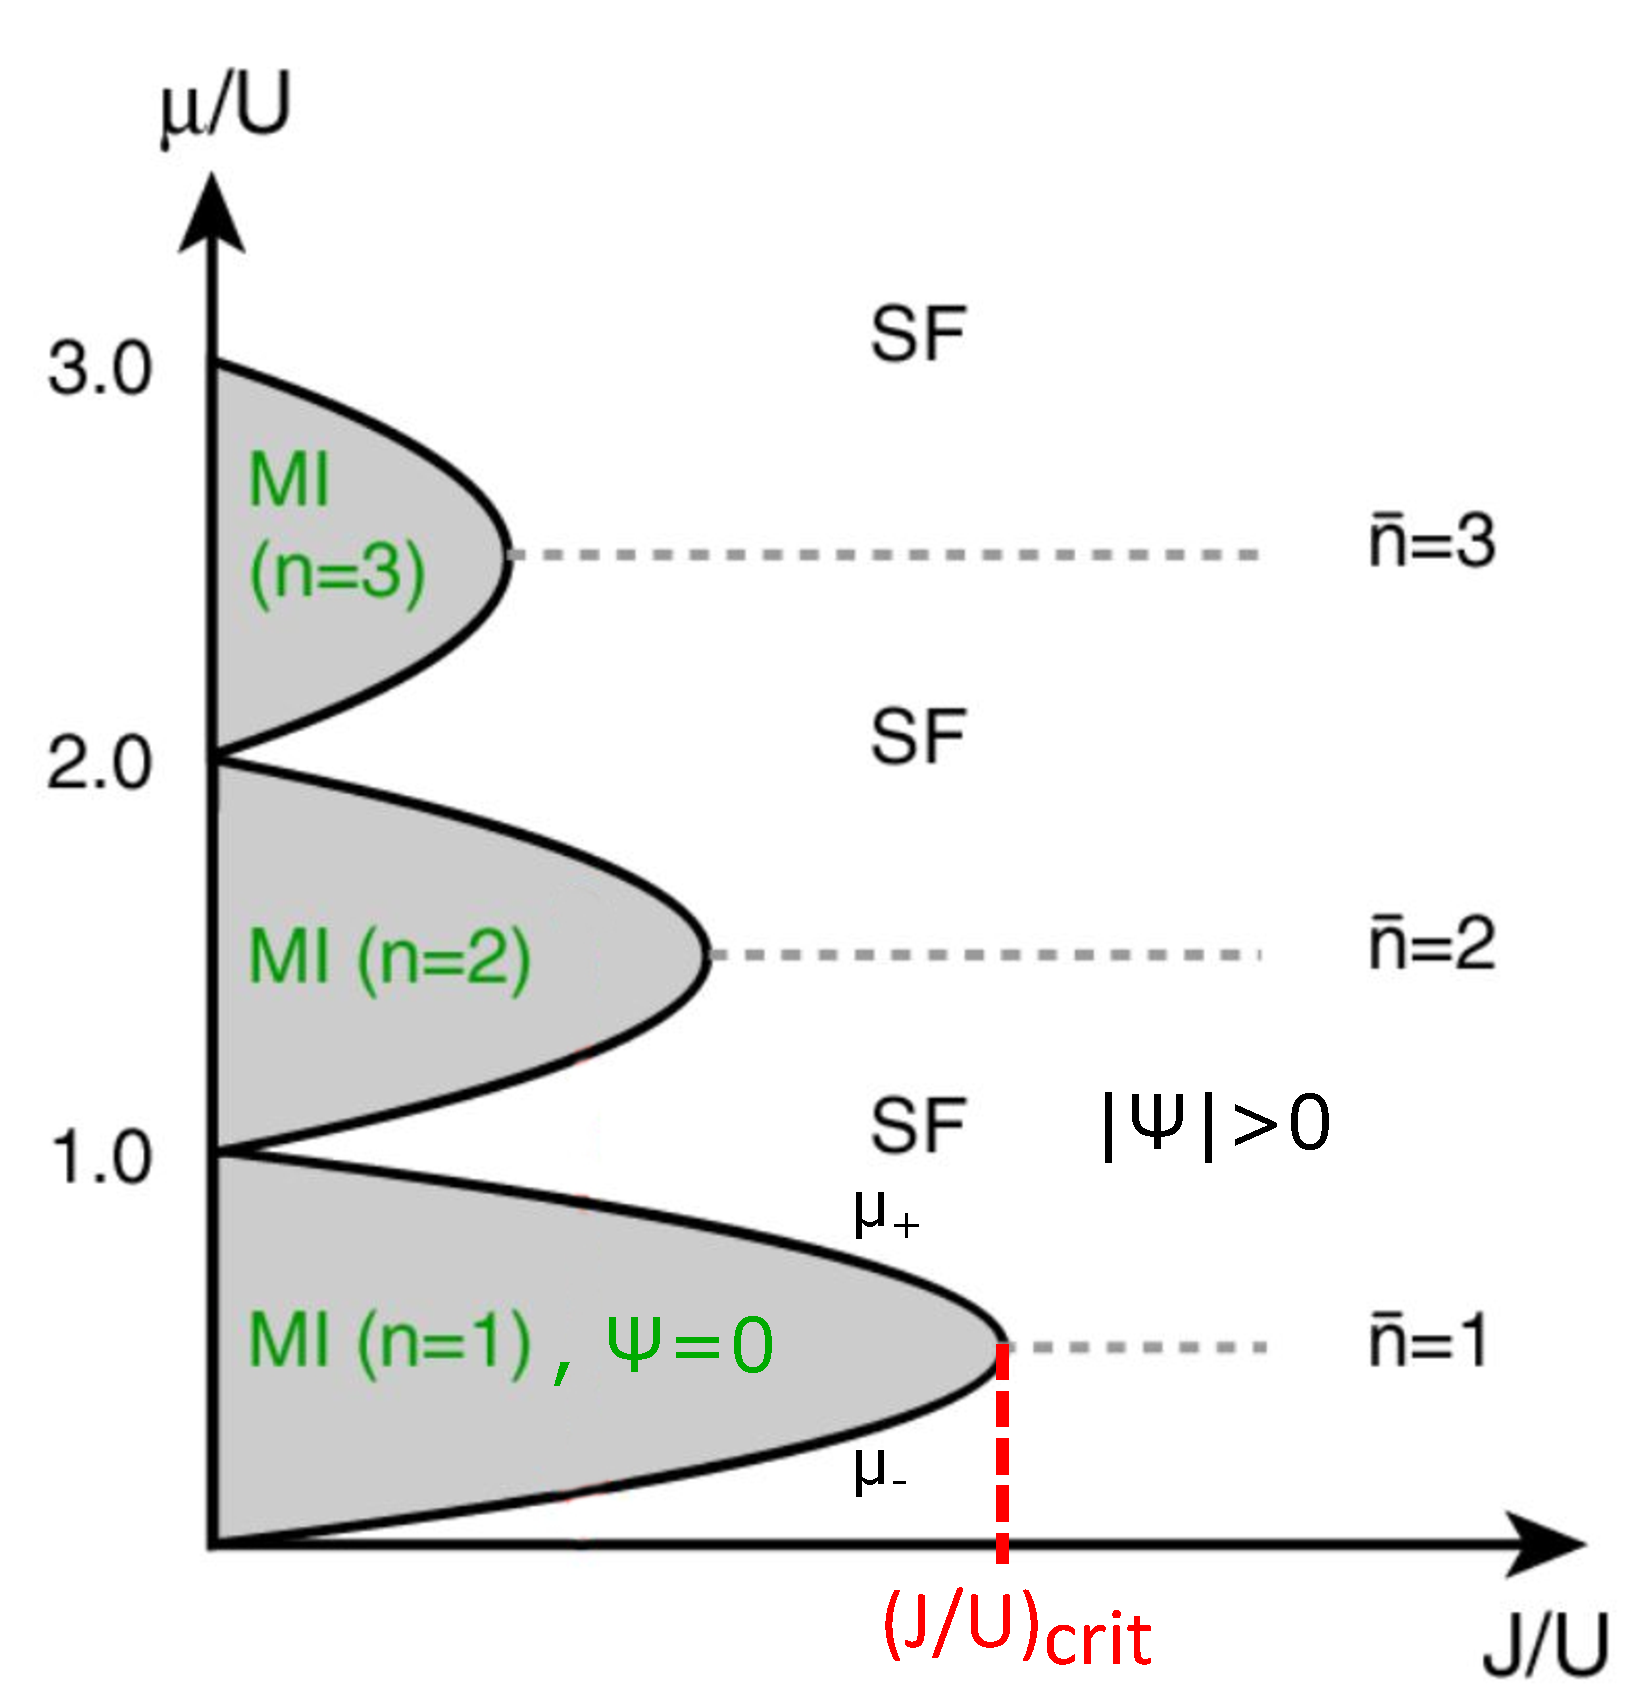
\includegraphics[width = 0.5\textwidth]{Figures/SFMottPhase.pdf}
	\label{fig:SFMOTT}
	\caption{\textit{Phase diagram of Bose-Hubbard model for T = 0. Grey areas mark the Mott Insulator phase for different number of particles per site, while white regions mark the superfluid phase. \cite{greiner}}}
\end{figure}
The $\mu_{\pm}$ curves encloses the region where the system is in the Mott Insulating phase. $(1/\bar{U})_{crit} = (J/U)_{crit}$ can be read off the graph from the point, where the two curves $\mu_{\pm}$ meet. As mentioned earlier, no fluctuations take place in the Mott Insulator, whereby the particle number per site is well defined, while it for the superfluid can take many values. As the chemical potential increases each site can accommodate more particles as long as the increase in chemical potential compensates the increased energy due to interactions between the particles.\\
The mean-field solution of the Bose-Hubbard model is only an approximation, which proves quite inaccurate for one dimension. This is seen when comparing the critical ratio for the mean-field approach, $\left( U/J \right)_{crit}^{MF,1D} = 11.66$, with numerical results computed using the DMRG method, $\left( U/J \right)_{crit}^{DMRG,1D} = 3.37$, \cite{Kuhner2000}. Nevertheless, it gives a good intuitive feeling of the physics taking place and how one can describe them without resorting to diagonalizing the Hamiltonian.\\
\chapter{Matrix Product States} \label{chap:MPS}
Numerical analysis of quantum many-body systems using exact diagonalisation is highly limited by system size. Due to the large number of possible configurations in a many-body system and entanglement coupling various degrees of freedom, the Hilbert space grows too large for exact methods to search.
Consider the Bose-Hubbard model described in eq. \eqref{BHhamil}. The dimension of the corresponding Hilbert space is
\begin{equation}
	D_{\mathcal{H}} = \frac{(L+N_p -1)!}{N_p ! (L-1)!} \; ,
\end{equation}
where $L$ is the number of sites, and $N_p$ is the number of particles. For unit occupancy, $N_p / L = 1$, the Hilbert space grows exponentially with the system size \cite{Dong}. Therefore, descriptions using exact diagonalisation are only possible for small systems.
Matrix product states parameterize the quantum states through a product of tensors, which can be depicted as a network. Decomposing the state as an explicitly contracted network of tensors enables efficient application of operators. Furthermore, the scaling of entanglement within a matrix product state is very different to the original state, as MPS follow an area law, whereby only a tiny corner of the Hilbert space has to be considered when searching for ground states \cite{Cramer}.\\
This chapter will cover the basics of matrix product states including their construction and freedom of gauges called canonical forms \cite{schollwock}. Furthermore, the generalization of MPS to operators called matrix product operators are introduced along with their applications. Algorithms involving matrix products states such as the DMRG method \cite{White1992,White1993} are introduced in the following chapter.


\section{Entanglement in Quantum Systems and Area Laws}
Entanglement is a fundamental property of quantum mechanics responsible for correlating different degrees of freedom within a quantum system. Thus, the individual parts of a quantum system can not be described alone, as entanglement with the remainder of the system has to be taken into consideration. This drastically complicates any description of the system, which is why exact descriptions of many-body systems are almost impossible.\\
The measure of entanglement within a quantum many-body system is the entanglement entropy, although it is often more instructive to look at the bipartite entanglement entropy, which measures the entanglement between two partitions of the system.
Consider a bipartition of the Hilbert space $\mathcal{H} = \mathcal{H}_A \otimes \mathcal{H}_B$. A state $\ket{\psi} \in \mathcal{H}$ can be decomposed using the \textit{Schmidt decomposition} as
\begin{equation}
	\ket{\psi} = \sum_{\alpha} \Lambda_{\alpha} \ket{\alpha}_A \otimes \ket{\alpha}_B \; ,
\end{equation}
where the states $\{ \ket{\alpha}_{A(B)} \}$ form an orthonormal basis of $\mathcal{H}_{A(B)}$, and $\Lambda_{\alpha} \ge 0$ are the Schmidt coefficients fulfilling $\sum_{\alpha} \Lambda_{\alpha}^2 = 1$ \cite{Pathak2013}. If only one term contributes to the Schmidt decomposition, the state is a product state i.e. the two parts of the Hilbert space are not mutually entangled. More terms implies that the state is entangled. From the Schmidt decomposition one can determine the reduced density matrix
\begin{equation}
	\rho_A = \Tr _B \ket{\psi}\bra{\psi} = \sum_{\alpha} \Lambda_{\alpha}^2 \ket{\alpha}_A \bra{\alpha}_A \; ,  
\end{equation}
by tracing out the subsystem $B$. 
From the Schmidt decomposition one can determine the entanglement entropy of the bipartition, which is defined as the von-Neumann entropy, $S$, of the reduced density matrix given by \cite{Pathak2013}
\begin{equation}
	S = - \sum_{\alpha} \Lambda_{\alpha}^2 \log \Lambda_{\alpha}^2 \; .
\end{equation}
Quite often, one is not concerned with the actual entanglement entropy of the system, but rather how it scales when the region in question grows in size. It is natural to assume that the entanglement entropy scales with  the \textit{volume} of the system, since this is the case for thermal systems. However, ground states of quantum many-body systems often follow an \textit{area law}, meaning that the scaling of the entropy is linear in the boundary area of the region. This is especially the case for systems with a gapped and local Hamiltonian \cite{Cramer}.\\
In a one dimensional lattice the boundary of a bipartition is constant in size independently of where the cut is made. Hence, the entropy will be bounded by a constant independent of the size of both the system and the subsystem, if the system follows an area law. This can be understood intuitively, as only degrees of freedom within the correlation length, $\xi$, of the boundary will be entangled, no matter where in the system the boundary is present \cite{Hastings2007}.\\
This observation is the key to the success of numerical computations for one-dimensional systems, as one has to consider only a small region of the Hilbert space when performing a variational search for the ground state. A highly efficient way of describing one dimensional systems is through Matrix Product States (MPS), which follow an area law by default, as they are constructed through a series of Schmidt decompositions.


\section{Construction of an MPS} \label{sec:construct_MPS}
Matrix products states are parametrisations of one dimensional quantum states through a product of tensors. This parametrisation is especially intuitive for lattice systems, as each lattice site can be represented by a single tensor. These tensors have two different kinds of indices; \textit{physical indices}, $j$, which corresponds to the local, physical states at a given site, and \textit{bond indices}, $\alpha$, which serves to connect neighbouring sites. Tensors can be merged by contracting the bond connecting them, which is done by summing over their common index. Equations involving matrix product states tend to grow quite long, whereby they often are described through diagrams. In the diagrammatic representation the physical indices are marked by vertical legs, while bond indices are marked by horisontal legs. When two tensors are connected by a leg, it means that the corresponding bond is contracted. Further details and examples regarding tensor diagrams can be found in Appendix \ref{chap:diagrams}.\\

Consider a chain of $L$ sites with each site having a $d$-dimensional local Hilbert space $\{ \ket{j_n} \}$, where $n = 1, \ldots, L$. An arbitrary quantum state of this system reads
\begin{equation}
	\ket{\psi} = \sum_{j_1, \ldots, j_L} c_{j_1 \ldots j_L} \ket{j_1, \ldots, j_L} \; .
	\label{eq:arbstate}
\end{equation}
This description of a general state can be parametrised to the MPS form by applying successive Schmidt decomposition. However, in practice this is done through Singular Value Decompositions (SVD), as these are faster to perform numerically. The two approaches are equivalent, as the singular value decomposition is essentially a restatement of the Schmidt decomposition CITE.
Through an SVD, an arbitrary matrix, $A$, of dimensions $(M \times N)$ can be decomposed into three matrices
\begin{equation}
	A = U S V^{\dag} \; .
\end{equation}
These matrices have the following properties \cite{schollwock}:
\begin{itemize}
\item
$U$ is of dimension $(M \times \min(M,N))$ and has orthonormal columns, meaning $U^{\dag}U = I$. If $M \leq N$, then it is also unitary $U U^{\dag} = I$.

\item
$S$ is a positive, diagonal $(\min(M,N) \times \min(M,N))$ matrix. The diagonal elements are singular values, and the number of non-zero entries is the Schmidt rank of $A$.

\item
$V^{\dag}$ is of dimension $(\min(M,N) \times N)$ and has orthonormal rows, meaning $V^{\dag}V = I$. If $M \geq N$, then it is also unitary $V V^{\dag} = I$.
\end{itemize} 
From the general state of eq. \eqref{eq:arbstate} an MPS can be constructed through the following steps:
\begin{enumerate}
\item
The $d^L$-dimensional vector $c_{j_1 \ldots j_L}$ is reshaped into a $(d \times d^{L-1})$ matrix $\Psi_{j_1 , (j_2 \ldots j_L)}$. Performing an SVD on $\Psi$ yields
\begin{equation}
	c_{j_1 \ldots j_L} = \Psi_{j_1 , (j_2 \ldots j_L)} = \sum_{\alpha_1}^{d} U_{j_1 , \alpha_1} S_{\alpha_1 , \alpha_1} (V^{\dag})_{\alpha_1 , (j_2 \ldots j_L)} = \sum_{\alpha_1}^{d} A_{\alpha_1}^{j_1} \Psi_{(\alpha_1 j_2),(j_3 \ldots j_L)} \; ,
\end{equation}
where $U$ has been reshaped into $d$ row vectors $A^{j_1}$ with entries $A_{\alpha_1}^{j_1} = U_{j_1 , \alpha_1}$. In this notation $A_{\alpha_1}^{j_1}$ is a tensor with physical indices $j_1$ and bond indices $\alpha_1$. Furthermore, $S$ and $V^{\dag}$ has been multiplied and reshaped into a $(d^2 \times d^{L-2})$ matrix, $\Psi_{(\alpha_1 j_2),(j_3 \ldots j_L)}$.

\item
The new matrix $\Psi_{(\alpha_1 j_2),(j_3 \ldots j_L)}$ is subjected to an SVD decomposition
\begin{equation}
	c_{j_1 \ldots j_L} = \sum_{\alpha_1}^{d} \sum_{\alpha_2}^{d^2} A_{\alpha_1}^{j_1} U_{(\alpha_1 j_2) , \alpha_2} S_{\alpha_2 , \alpha_2} (V^{\dag})_{\alpha_2 , (j_3 \ldots j_L)} = \sum_{\alpha_1}^{d} \sum_{\alpha_2}^{d^2} A_{\alpha_1}^{j_1} A_{\alpha_1 , \alpha_2}^{j_2} \Psi_{(\alpha_2 j_3),(j_4 \ldots j_L)} \; ,
\end{equation}
where $U$ has been decomposed into $d$ matrices $A^{j_2}$ with entries $A_{\alpha_1 , \alpha_2}^{j_2} = U_{(\alpha_1 j_2) , \alpha_2}$. The matrix $\Psi_{(\alpha_2 j_3),(j_4 \ldots j_L)}$ has dimensions $(d^3 \times d^{L-3})$ and is yet again a product of the matrices $S$ and $V^{\dag}$ from the SVD.

\item
The procedure detailed in the two previous steps is continued throughout the chain leaving 
\begin{equation}
	c_{j_1 \ldots j_L} = \sum_{\alpha_1 , \ldots , \alpha_{L-1}} A_{\alpha_1}^{j_1} A_{\alpha_1 , \alpha_2}^{j_2} \ldots A_{\alpha_{L-2} ,\alpha_{L-1}}^{j_{L-1}} A_{\alpha_{L-1} ,\alpha_{L}}^{j_{L}} \equiv A^{j_1} A^{j_2} \ldots A^{j_{L-1}} A^{j_{L}} \; ,
\end{equation}
where the sum can be recognized as a matrix multiplication allowing a neater notation.
\end{enumerate}
\begin{figure}[h!]
	\centering
	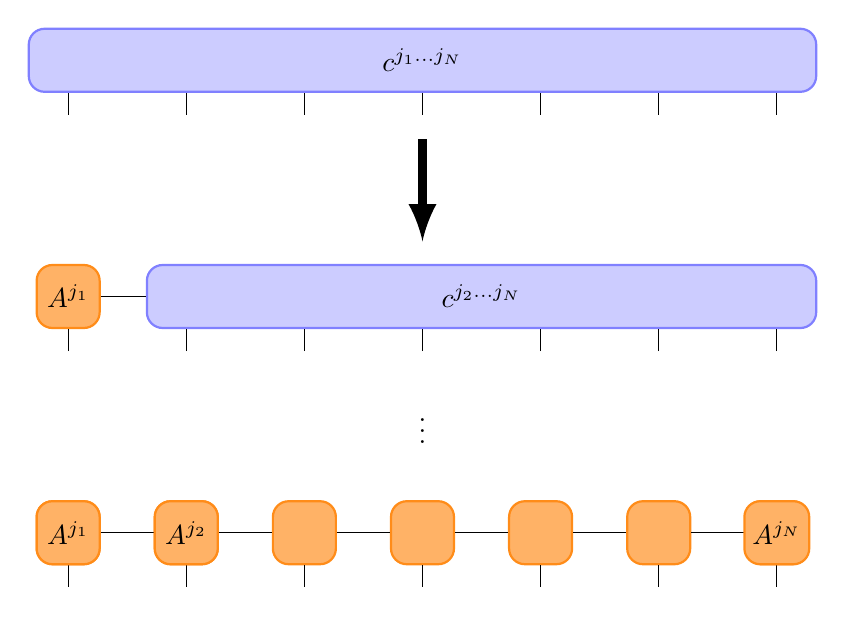
\begin{tikzpicture}[inner sep=1mm]
	\def \numb {7};
	\def \hdist {1.5};
	\def \wid {10};
	\def \wids {8.5};

	\node[tensor, minimum width=\wid cm] (tens1) at (\wid/2 +1, 0) {$c^{j_1 \ldots j_N}$};
	
	\foreach \i in  {1,...,\numb} {
		\node (\i) at (\i*\hdist, -0.8) {};
		\draw[-] (\i) -- (\i |-  tens1.south);	
	};
	
	\draw[->, line width=1.25mm] (\wid/2 +1,-1) -- (\wid/2 +1,-2.3);
	
	\node[tensorl] (blok1) at (1*\hdist, -3) {$A^{j_1}$};
	\node[tensor, minimum width=\wids cm] (tens2) at (\wids/2 +2.5, -3) {$c^{j_2 \ldots j_N}$};
	
	\foreach \i in  {2,...,\numb} {
		\node (\i) at (\i*\hdist, -3.8) {};
		\draw[-] (\i) -- (\i |-  tens2.south);	
	};
	\node (node1) at (1*\hdist, -3.8) {};
	\draw[-] (node1) -- (blok1);
	\draw[-] (tens2) -- (blok1);
	
	\node (dots) at (\wid/2 +1, -4.6) {\vdots};
	
	\foreach \i in  {1,...,\numb} {
		\node[tensorl] (t\i) at (\i*\hdist, -6) {};
		\node (\i) at (\i*\hdist, -6.8) {};
		\draw[-] (t\i) -- (\i);	
	};
	\foreach \i in  {1,...,6} {
		\pgfmathtruncatemacro{\iplusone}{\i + 1};
		\draw[-] (t\i) -- (t\iplusone);	
	};
	
	\node[tensorl] (lab1) at (1*\hdist, -6) {$A^{j_1}$};
	\node[tensorl] (lab2) at (2*\hdist, -6) {$A^{j_2}$};
	\node[tensorl] (labN) at (\numb*\hdist, -6) {$A^{j_N}$};
	
\end{tikzpicture}
	\caption{\textit{Diagrammatic representation of the construction of a left-canonical MPS from an arbitrary quantum state through successive SVD's.}}
	\label{fig:MPSbuild}
\end{figure}
The construction of an MPS is illustrated in figure \ref{fig:MPSbuild}. Thereby, the original state (equation \ref{eq:arbstate}) can be written as a matrix product state in the form \cite{schollwock}
\begin{equation}
	\ket{\psi} = \sum_{j_1, \ldots, j_L} A^{j_1} A^{j_2} \ldots A^{j_{L-1}} A^{j_{L}} \ket{j_1, \ldots, j_L} \; .
	\label{eq:MPS_LC} 
\end{equation}
\\
Due to the dimensions of the components of an SVD, the dimensions of the matrices $A^{j_n}$ follow a pyramid-like structure $(1 \times d ),(d \times d^2) , \ldots , (d^{L/2 -1} \times d^{L/2}) , (d^{L/2} \times d^{L/2 -1 }), \ldots , (d \times 1)$, where $L$ is taken as even for simplicity. Hence, the matrix dimensions increase exponentially making exact computations practically impossible. However, certain simplifications can be made, which greatly reduces computational time without sacrificing much precision. First, one only needs to keep the non-zero, singular values of the matrices $S$, thus reducing the dimensional factor from $d$ to $r_n$, where $r_n \leq d$ is the Schmidt rank of the n'th decomposition. Secondly, as discussed earlier, only a few terms is needed to accurately describe entanglement across bonds. Therefore, the matrices $S$, $U$ and $V$ can be truncated keeping only the $D$ largest singular values, as these contribute the most to the state. Thus, the dimension of the matrices will cap at $D$: $(1 \times d ),(d \times d^2) , \ldots , (d^{n} \times D) , (D \times D), \ldots , ( D \times d^{n}) \ldots  (d \times 1)$, avoiding the otherwise exponential dimensional growth \cite{EntropyScaling}. The amount of singular values needed to be kept in order to produce an accurate approximation of the state is highly dependent of the system. Thus, one often need to perform the same calculation for various values of $D$, in order to gauge how much the matrices can be truncated.


\section{Canonical Forms}
\label{sec:canonical}
The MPS described in equation \ref{eq:MPS_LC} is not unique, as writing 
\begin{equation}
	\tilde{A}^{j_n} = X_{n-1} A^{j_n} X_{n}^{-1}
\end{equation}
describes the same state using different matrices. This gauge freedom allows expressing the MPS in whichever way is most convenient, which can greatly reduce the effort of applying operators and calculating overlaps. By choosing a gauge, the MPS is brought into a \textit{canonical form} \cite{Vidal2007}.

\subsection{Left-canonical matrix product state}
The process of constructing an matrix product state detailed in Section \ref{sec:construct_MPS} brings the MPS in a \textit{left-canonical} form. This implies that all the matrices are left-normalized, such that
\begin{equation}
	\sum_{j_n} A^{j_n \dag} A^{j_n} = I \; .
	\label{eq:LC_ident}
\end{equation}
The left-normalization is a consequence of the matrix $U$ (from the SVD) fulfilling $U^{\dag}U = I$. Since the matrices $A^{j_n}$ are reshaped from $U$, these properties persists
\begin{align*}
	\delta_{\alpha_n , \alpha_n'} &= \sum_{\alpha_{n-1} j_n} (U^{\dag})_{\alpha_n , (\alpha_{n-1} j_n)} U_{(\alpha_{n-1} j_n), \alpha_n'} \\
	 &= \sum_{\alpha_{n-1} j_n} (A^{j_n \dag})_{\alpha_n , \alpha_{n-1}} A_{\alpha_{n-1}, \alpha_n'}^{j_n} \\
	 &= \sum_{j_n} \left( A^{j_n \dag} A^{j_n} \right)_{\alpha_{n} . \alpha_n'}
\end{align*} 
\begin{figure}[h!]
	\centering
	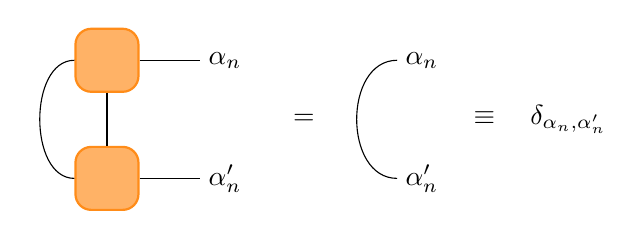
\begin{tikzpicture}[inner sep=1mm]
	\def \vdist {1.5};

	\node[tensorl] (tens1) at (1,0) {};
	\node[tensorl] (tens2) at (1,-\vdist) {}; 
 	
	\node (index1) at (2.5,0) {$\alpha_n$};
	\node (index2) at (2.5,-\vdist) {$\alpha_n '$}; 	
 	
 	\draw[-] (tens1) -- (tens2);
	\draw[-] (tens1) -- (index1);
	\draw[-] (tens2) -- (index2); 	
    \draw[-] (tens1.west) .. controls (0, 0) and (0, -\vdist) .. (tens2.west);
    
    
    \node (eq) at (3.5,-\vdist/2) {$=$};
    
    
 	\node (dummy1) at (5,0) {$\alpha_n$};
 	\node (dummy2) at (5,-\vdist) {$\alpha_n '$};
    
    \draw[-] (dummy1.west) .. controls (4, 0) and (4, -\vdist) .. (dummy2.west);
    
    \node (equiv) at (6.5,-\vdist/2) {$\equiv \quad \delta_{\alpha_n , \alpha_n '}$};
\end{tikzpicture}
	\caption{\textit{Contraction over the left index (shown as the arc) and the physical index of two left-normalised matrices. The result is $\delta_{\alpha_n , \alpha_n'}$, adding the n'th site to the contraction of all previous sites to the left.}}
	\label{fig:leftNorm}
\end{figure}
Figure \ref{fig:leftNorm} illustrates a contraction of the bonds connecting two left-normalised matrices. As this contraction results in the identity per definition, one can contract left-normalised matrices without any explicit calculation. The explicit contraction is displayed diagrammatically through an arc, which is equivalent to an identity-tensor with two bond indices. 


\subsection{Right-canonical matrix product state}
One could also have built a a right-canonical MPS from eq. \eqref{eq:arbstate}, had one performed the SVDs from other side of the chain. Constructing the MPS from the right implies multiplying $U$ and $S$ into the new $\Psi$-matrix, and reshaping $(V^{\dag})_{(\alpha_{n-1} j_n), \alpha_n}$ into matrices $B_{\alpha_{n-1} , \alpha_n}^{j_n}$. Hence, the right-canonical form of the MPS of eq. \eqref{eq:MPS_LC} reads
\begin{equation}
	\ket{\psi} = \sum_{j_1, \ldots, j_L} B^{j_1} B^{j_2} \ldots B^{j_{L-1}} B^{j_{L}} \ket{j_1, \ldots, j_L} \; .
\label{eq:MPS_RC}	 
\end{equation}
In this form all the matrices are right-normalized, whereby 
\begin{equation}
	\sum_{j_n} B^{j_n} B^{j_n \dag} = I \; .
	\label{eq:RC_ident}
\end{equation}
Note the reverse ordering of the matrix product compared to the left-normalized case. Figure \ref{fig:rightNorm} illustrates two right-normalised matrices contracted over their physical index.
\begin{figure}[h!]
	\centering
	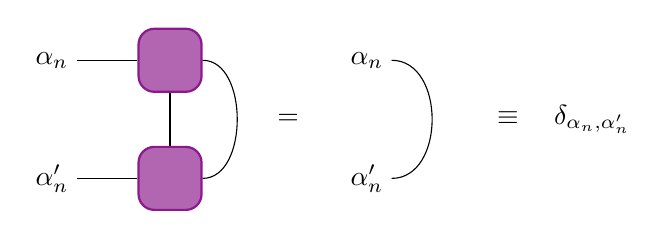
\begin{tikzpicture}[inner sep=1mm]
	\def \vdist {1.5};
	
	\node[tensorr] (tens1) at (2.5,0) {};
	\node[tensorr] (tens2) at (2.5,-\vdist) {}; 
 	
	\node (index1) at (1,0) {$\alpha_n$};
	\node (index2) at (1,-\vdist) {$\alpha_n '$}; 	
 	
 	\draw[-] (tens1) -- (tens2);
	\draw[-] (tens1) -- (index1);
	\draw[-] (tens2) -- (index2); 	
    \draw[-] (tens1.east) .. controls (3.5, 0) and (3.5, -\vdist) .. (tens2.east);
    
    
    \node (eq) at (4,-\vdist/2) {$=$};
    
    
 	\node (dummy1) at (5,0) {$\alpha_n$};
 	\node (dummy2) at (5,-\vdist) {$\alpha_n '$};
    
    \draw[-] (dummy1.east) .. controls (6, 0) and (6, -\vdist) .. (dummy2.east);
    
    \node (equiv) at (7.5,-\vdist/2) {$\equiv \quad \delta_{\alpha_n , \alpha_n '}$};
\end{tikzpicture}
	\caption{\textit{Contraction over the right index (shown as the arc) and the physical index of two right-normalised matrices.}}
	\label{fig:rightNorm}
\end{figure}


\subsection{Mixed-canonical matrix product state}
In practice one rarely finds use for a purely left- or right-canonical MPS. However, combining the two canonical forms listed above yields the mixed-canonical form. The mixed-canonical results in a natural bi-partitioning of the system into a Schmidt decomposition, and it is especially useful for measuring local properties of the state \cite{schollwock}.\\
Consider the procedure of building an MPS in the left-canonical form, where $c_{j_1 \ldots j_L}$ has been decomposed from the left up until site $n$
\begin{equation}
	c_{j_1 \ldots j_L} = \sum_{\alpha_n} \left( A^{j_1} \ldots  A^{j_n} \right) _{\alpha_n} S_{\alpha_n , \alpha_n} (V^{\dag})_{\alpha_n , (j_{n+1} \ldots j_L)} \; .
\end{equation}
By reshaping $V^{\dag}$  into the matrix $\Psi_{(\alpha_n j_{n+1} \ldots j_{N-1}),j_N}$, one can initiate a successive decomposition from the right, resulting in a set of right-normalized matrices. The final result reads
\begin{equation}
	c_{j_1 \ldots j_N} = A^{j_1} \ldots A^{j_n} S B^{j_{n+1}} \ldots B^{j_L} \; ,
	\label{eq:mixedCanon}
\end{equation}
which is illustrated in figure \ref{fig:MixedCanonical1}.
\begin{figure}[h!]
\centering % <-- add this
\begin{subfigure}[b]{0.47\textwidth}
	\caption{}  	
  	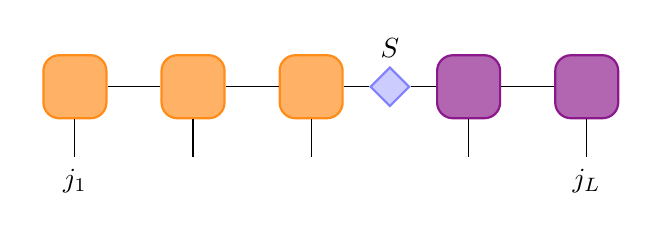
\begin{tikzpicture}[inner sep=1mm]
	\def \hdist {1.5};
	\def \numb {5};
	\def \vleg {1};
	\def \NL {3};
	
	\node[minimum height=0.5 cm] (frame) at (1 ,0.5) {};

	\foreach \i in  {1,...,\NL} {
		\node[tensorl] (\i) at (\i*\hdist, 0) {};
		\node (index\i) at (\i*\hdist, -\vleg) {};
		\draw[-] (\i) -- (index\i);	
	};
	
	\foreach \i in  {1,...,2} {
		\pgfmathtruncatemacro{\iplusone}{\i + 1};
		\draw[-] (\i) -- (\iplusone);
	};
	
	\foreach \i in  {5,...,6} {
		\node[tensorr] (\i) at (\i*\hdist-\hdist/1.5, 0) {};
		\node (index\i) at (\i*\hdist-\hdist/1.5, -\vleg) {};
		\draw[-] (\i) -- (index\i);	
	};

	\foreach \i in  {5,...,5} {
		\pgfmathtruncatemacro{\iplusone}{\i + 1};
		\draw[-] (\i) -- (\iplusone);
	};
	
	\node[matrix, label={$S$}] (S) at (\NL*\hdist+\hdist/1.5,0) {};
	\draw[-] (\NL) -- (S);
	\draw[-] (S) -- (5);
	\node (indexL) at (1*\hdist, -\vleg -0.2) {$j_1$};
	\node (indexR) at (6*\hdist-\hdist/1.5 , -\vleg -0.2) {$j_L$};			
\end{tikzpicture}
	\label{fig:MixedCanonical1}
\end{subfigure}
\hspace{5mm}
\begin{subfigure}[b]{0.47\textwidth}    
	\caption{}  	
  	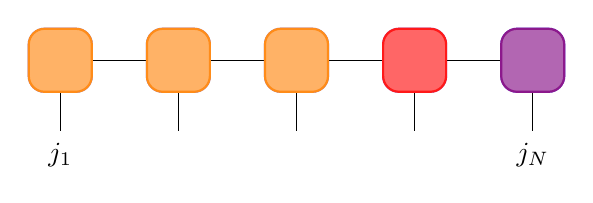
\begin{tikzpicture}[inner sep=1mm]
	\def \hdist {1.5};
	\def \numb {5};
	\def \vleg {1};
	\def \NL {3};

	\foreach \i in  {1,...,\numb} {
		\node[tensor] (\i) at (\i*\hdist, 0) {};
		\node (index\i) at (\i*\hdist, -\vleg) {};
		\draw[-] (\i) -- (index\i);	
	};
	
	\foreach \i in  {1,...,4} {
		\pgfmathtruncatemacro{\iplusone}{\i + 1};
		\draw[-] (\i) -- (\iplusone);
	};
	
	\foreach \i in  {1,...,\NL} {
		\node[tensorl] (\i) at (\i*\hdist, 0) {};
	};
	
	\node[tensorc] (C) at (\numb*\hdist-\hdist, 0) {};
	\node[tensorr] (R) at (\numb*\hdist, 0) {};


	\node (indexL) at (1*\hdist, -\vleg -0.2) {$j_1$};
	\node (indexR) at (\numb*\hdist, -\vleg -0.2) {$j_N$};		
\end{tikzpicture}
	\label{fig:MixedCanonical2}
\end{subfigure}
\caption{\textit{Two variants of the mixed-canonical form of an MPS. The form \textbf{(a)} retains the matrix S originating from the SVD, whereby the MPS is directly brought into the form of a Schmidt decomposition. Multiplying S into either ites left or right neighbour creates the form \textbf{(b)}, which has a central site containing the normalization of the entire state. The form \textbf{(b)} is well suited for measuring local properties of the state.}}
\end{figure}
In the mixed-canonical form the Schmidt decomposition can be read directly from the form of the MPS by introducing the vectors
\begin{align}
 	\ket{\alpha_n}_A \; &= \; \sum_{j_1 , \ldots , j_n} \left( A^{j_1} \ldots A^{j_n} \right)_{1,\alpha_n} \ket{j_1 , \ldots , j_n}  \label{eq:mixedA} \\
 	\ket{\alpha_n}_B \; &= \; \sum_{j_{n+1} , \ldots , j_L} \left( B^{j_{n+1}} \ldots B^{j_L} \right)_{\alpha_n , 1} \ket{j_{n+1} , \ldots , j_L} \; , \label{eq:mixedB}
\end{align}
whereby the state can be written in the form
\begin{equation}
	\ket{\psi} = \sum_{\alpha_n} S_{\alpha_n , \alpha_n} \ket{\alpha_n}_A \ket{\alpha_n}_B \; . \label{eq:MixedFormA}
\end{equation}
In order for eq. \eqref{eq:MixedFormA} to be considered a Schmidt decomposition, the matrix $S$ must fulfill $\sum_{\alpha_n} (S_{\alpha_n , \alpha_n})^2 = 1$, which is fulfilled by default by the SVD. Furthermore, the states $\ket{\alpha_n}_A$ and $\ket{\alpha_n}_B$ have to be orthonormal respectively, which they are by construction.\\
Another useful version of the mixed-canonical form is depicted in figure \ref{fig:MixedCanonical2}, where the matrix $S$ of eq. \eqref{eq:mixedCanon} has been multiplied unto the matrix to either the left or right of it. The result is a central cite, which is neither left- nor right-normalized, but instead contains the normalization of the entire state. Overlaps can expectation values can be computed very efficiently using the mixed-canonical form, as most of the tensor network can be explicitly contracted due to the normalization. 
 

\subsection{Bringing a matrix product state into canonical form}
The previous examples of canonical forms were realised during the construction of the matrix product states. However, any arbitrary MPS can be be brought into a canonical form through a series of SVD's, again exploiting the left-/right-normalization of the resulting matrices.\\
Consider a general MPS
\begin{equation}
	\ket{\psi} = \sum_{j_1 , \ldots , j_L} \sum_{\alpha_1 , \ldots } M_{1 , \alpha_1}^{j_1} M_{\alpha_1 , \alpha_2}^{j_2} M_{\alpha_2 , \alpha_3}^{j_3} \ldots \ket{j_1 , \ldots , j_L} \; , 
	\label{eq:generalMPS}
\end{equation}
which has to be brought into a left-canonical form. By grouping the physical and left (row) index of $M_{1 , \alpha_1}^{j_1}$, one can reshape the tensor into a single matrix, $M_{(j_1 , 1) , \alpha_1}$. Applying an SVD yields $M = A S V^{\dag}$, where $A^{\dag} A = I$, such that $A$ is left-normalized as desired. Thus, the left-normalisation of the first tensor of the MPS reads
\begin{align}
\ket{\psi} = & \; \sum_{j_1 , \ldots , j_L} \sum_{\alpha_1 , \ldots } M_{(j_1 , 1) , \alpha_1} M_{\alpha_1 , \alpha_2}^{j_2} M_{\alpha_2 , \alpha_3}^{j_3} \ldots \ket{j_1 , \ldots , j_L} \nonumber \\
= & \; \sum_{j_1 , \ldots , j_L} \sum_{\alpha_1 , \ldots } \sum_{s_1} A_{(j_1 , 1) , s_1} S_{s_1 , s_1} V_{s_1 , \alpha_1}^{\dag} M_{\alpha_1 , \alpha_2}^{j_2} M_{\alpha_2 , \alpha_3}^{j_3} \ldots \ket{j_1 , \ldots , j_L} \nonumber \\
= & \; \sum_{j_1 , \ldots , j_L} \sum_{\alpha_1 , \ldots } \sum_{s_1} A_{1 , s_1}^{j_1} \left( S_{s_1 , s_1} V_{s_1 , \alpha_1}^{\dag} M_{\alpha_1 , \alpha_2}^{j_2} \right) M_{\alpha_2 , \alpha_3}^{j_3} \ldots \ket{j_1 , \ldots , j_L} \nonumber \\
= & \; \sum_{j_1 , \ldots , j_L} \sum_{\alpha_2 , \ldots } \sum_{s_1} A_{1 , s_1}^{j_1} \tilde{M}_{s_1 , \alpha_2}^{j_2} M_{\alpha_2 , \alpha_3}^{j_3} \ldots \ket{j_1 , \ldots , j_L} \; ,
\end{align}
where $\tilde{M}_{s_1 , \alpha_2}^{j_2} = \sum_{\alpha_1} S_{s_1 , s_1} V_{s_1 , \alpha_1}^{\dag} M_{\alpha_1 , \alpha_2}^{j_2}$. This procedure can be iterated through the entire chain, leaving the MPS in the left-canonical form \cite{schollwock}.\\
Likewise, an MPS can be brought into a right-canonical form by grouping the physical index with the right (column) index of $M$ yielding the SVD $M = U S B$, where $B B^{\dag} = I$. Thus, iterating through the chain from the right will produce a right-canonical MPS.

\section{Overlaps and Efficient Contractions}
Similarly to matrix multiplication, the number of computations need for contracting a string of tensors can be greatly reduced when performing the contractions in the right order. Consider the general case of two general states $\ket{\psi}$ and $\ket{\phi}$ described by the matrices $M$ and $\tilde{M}$. The overlap between these states reads
\begin{equation}
	\braket{\phi | \psi} = \sum_{j_1 , \ldots , j_L} \tilde{M}^{j_L \dag} \ldots \tilde{M}^{j_1 \dag} M^{j_1} \ldots M^{j_L} \; , 
	\label{eq:overlap}
\end{equation}
which is represented diagrammatically in figure \ref{fig:effCont}.
\begin{figure}[h!]
	\centering
	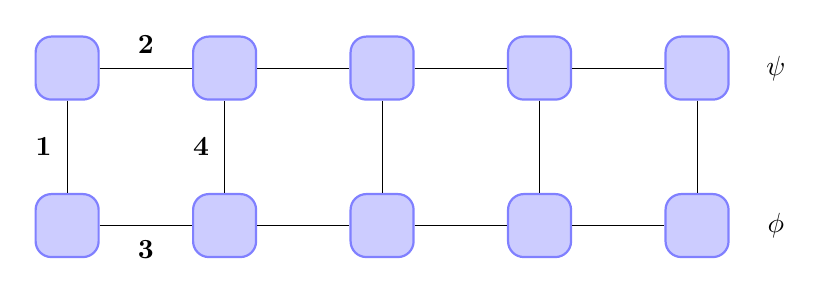
\begin{tikzpicture}[inner sep=1mm]
	\foreach \i in  {1,...,5} {
		\node[tensor] (t\i) at (\i*2-1, 0) {};
		\node[tensor] (b\i) at (\i*2-1, -2) {};
		\draw[-] (t\i) -- (b\i);	
	};
	\foreach \i in  {1,...,4} {
		\pgfmathtruncatemacro{\iplusone}{\i + 1};
		\draw[-] (t\i) -- (t\iplusone);
		\draw[-] (b\i) -- (b\iplusone);
	};
	
	\node (node1) at (0.7, -1) {\textbf{1}};
	\node (node2) at (2, 0.3) {\textbf{2}};
	\node (node3) at (2, -2.3) {\textbf{3}};
	\node (node4) at (2.7, -1) {\textbf{4}};
	
	\node (psi) at (10, 0) {$\ket{\psi}$};
	\node (phi) at (10, -2) {$\bra{\phi}$};
\end{tikzpicture}
	\caption{\textit{Efficient contraction of the overlap between two general states $\ket{\psi}$ and $\ket{\phi}$. By contracting the bonds in the specified order the number of multiplications is greatly reduced.}}
	\label{fig:effCont}
\end{figure}
The evaluation of the overlap can be drastically sped up by considering the optimal order of contractions, which corresponds to an optimal bracketing of eq. \eqref{eq:overlap}:
\begin{equation}
	\braket{\phi | \psi} = \sum_{j_L} \tilde{M}^{j_L \dag} \left( \ldots \left( \sum_{j_2} \tilde{M}^{j_2 \dag} \left( \sum_{j_1} \tilde{M}^{j_1 \dag} M^{j_1} \right) M^{j_2} \right) \ldots \right) M^{j_L} \; .
	\label{eq:optBrackets}
\end{equation}  
Within the innermost bracket a matrix is formed by multiplying a column and a row vector followed by the summation over the first physical index, $j_1$. In the remaining set of brackets three matrices are multiplied and the corresponding physical index is summed over. However, after the first contraction the complexity of the operation does not increase. Consider the worst case scenario of all the matrices being of dimension $(D \times D)$ with a local Hilbert space of dimension $d$. The total operational cost of the optimal contraction is $\mathrm{O}(L D^3 d)$ compared to otherwise exponential complexity of a random order of contractions \cite{schollwock}. The order of contractions described in eq. \eqref{eq:optBrackets} is illustrated in figure \ref{fig:effCont}.\\
When calculating a norm, $\braket{\psi | \psi}$, the canonical form of the MPS greatly reduces to computational time, as having an either left- or right-canonical MPS implies a norm of 1 without any contractions needed.

\section{Matrix Product Operators} \label{sec:MPO}
A Matrix Product Operator (MPO) is an operator expressed in the formalism of an MPS. Thereby, operators can be incorporated as part of the tensor networks, where they are evaluated by the contraction of bonds.\\
Consider a single coefficient of an MPS of the state general $\ket{\psi}$
\begin{equation}
	\braket{j_1 , \ldots , j_L | \psi} = \braket{\boldsymbol{j} | \psi} = M^{j_1} M^{j_2} \ldots M^{j_L} \; . 
\end{equation}
Expressing an operator $\hat{O}$ in the basis of the local states, one can write it in a similar manner
\begin{equation}
	\hat{O} = \sum_{\boldsymbol{j} , \boldsymbol{j'}} \ket{\boldsymbol{j}} \bra{\boldsymbol{j}} \hat{O} \ket{\boldsymbol{j'}} \bra{\boldsymbol{j'}} = \sum_{\boldsymbol{j} , \boldsymbol{j'}} W^{j_1 , j_1 '} W^{j_2 , j_2 '} \ldots W^{j_L , j_L '} \ket{\boldsymbol{j}} \bra{\boldsymbol{j '}} \; ,
	\label{eq:MPOrep}
\end{equation}
where the coefficients are $\bra{\boldsymbol{j}} \hat{O} \ket{\boldsymbol{j'}} = W^{j_1 , j_1 '} W^{j_2 , j_2 '} \ldots W^{j_L , j_L '}$. The operator matrices, $W^{j_n , j_n '}$, differ from the state matrices, $M$, as the representation of the operators needs both an ingoing and an outgoing physical index. The ingoing physical index is depicted graphically as an extra vertical leg. A pictorial representation of the operator $\hat{O}$ can be seen in figure \ref{fig:MPOchain}.
\begin{figure}[h!]
	\centering
	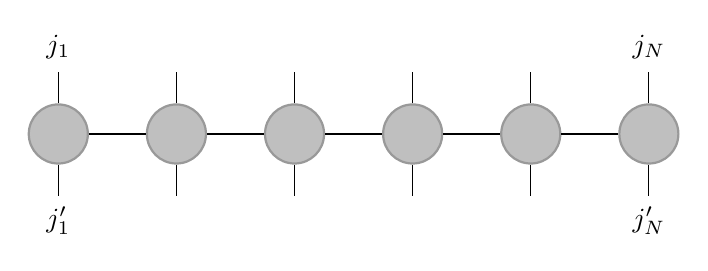
\begin{tikzpicture}[inner sep=1mm]
	\def \numb {6};	
	\def \hdist {1.5};
	
    \foreach \i in {1,...,\numb} {
        \node[operator] (\i) at (\i*\hdist, 0) {};
        \node (t\i) at (\i*\hdist, 0.9) {};
        \node (b\i) at (\i*\hdist, -0.9) {};
        
        \draw[-] (\i) -- (t\i);
        \draw[-] (\i) -- (b\i); 
    };
    
    \foreach \i in {1,...,5} {
        \pgfmathtruncatemacro{\iplusone}{\i + 1};
        \draw[-] (\i) -- (\iplusone);
    };
    
    \node (t1) at (\hdist, 1.1) {$j_1$};
    \node (b1) at (\hdist, -1.1) {$j_1 '$};
    \node (t\numb) at (\numb*\hdist, 1.1) {$j_N$};
    \node (b\numb) at (\numb*\hdist, -1.1) {$j_N '$};
\end{tikzpicture}
	\caption{\textit{An operator $\hat{O}$ expressed in the MPS form (MPO). The resulting matrix product operator has two physical indices marked by vertical lines, which corresponds to an ingoing and outgoing physical state.}}
	\label{fig:MPOchain}
\end{figure}

\subsection{Applying an MPO to an MPS}
Applying a matrix product operator to a matrix product state is simply a matrix multiplication, where the matching physical indices are summed over:
\begin{align}
	\hat{O} \ket{\psi} &=  \sum_{\boldsymbol{j},\boldsymbol{j'}} \sum_{\boldsymbol{\alpha},\boldsymbol{\beta}} \left( M_{1, \alpha_1}^{ j_1 '} M_{\alpha_1, \alpha_2}^{j_2 '} \ldots \right) \left( W_{1, \beta_1}^{j_1 ' , j_1 } W_{\beta_1, \beta_2}^{j_2 ', j_2 } \ldots \right) \ket{\boldsymbol{j}} \nonumber \\
&= \sum_{\boldsymbol{j},\boldsymbol{j'}} \sum_{\boldsymbol{\alpha},\boldsymbol{\beta}} \left( M_{1, \alpha_1}^{ j_1 '} W_{1, \beta_1}^{j_1 ' , j_1} \right) \left( M_{\alpha_1, \alpha_2}^{j_2 '}  W_{\beta_1, \beta_2}^{j_2 ' , j_2} \right) \ldots \ket{\boldsymbol{j}} \nonumber \\
&= \sum_{\boldsymbol{j}} \sum_{\boldsymbol{\alpha},\boldsymbol{\beta}} N_{(1,1),(\alpha_1 , \beta_1)}^{j_1} N_{(\alpha_1 , \beta_1),(\alpha_2 , \beta_2)}^{j_2} \ldots \ket{\boldsymbol{j}} \nonumber \\
&\equiv \sum_{\boldsymbol{j}} N^{j_1} N^{j_2} \ldots \ket{\boldsymbol{j}} \; = \; \ket{\phi}
\label{eq:optBracketsMPO}
\end{align} 
The result is a new MPS, $\ket{\phi}$, which is described by the matrices $N^{j_n}$ and is illustrated in figure \ref{fig:MPOcont}. These matrices have the dimensions of the product of the dimensions of the original MPS and MPO. Thus, applying an operator leaves the form of the MPS invariant but increases the matrix dimensions.
\begin{figure}[h!]
	\centering
	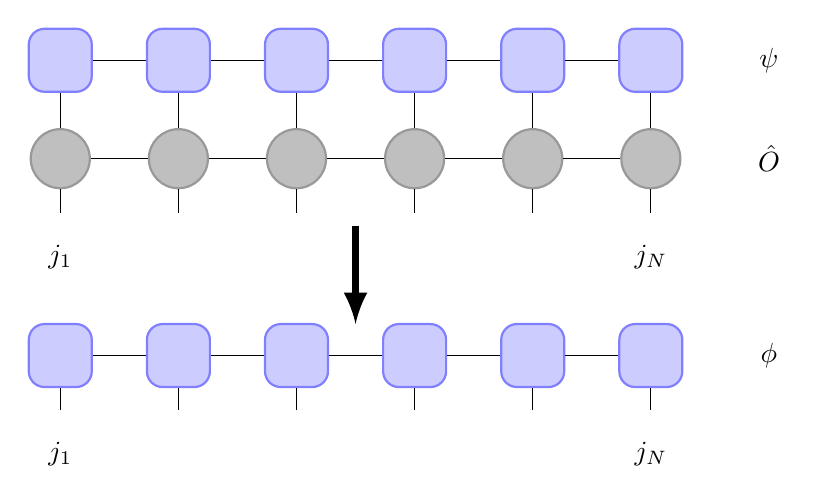
\begin{tikzpicture}[inner sep=1mm]
	\def \numb {6};
	\def \hdist {1.5};
	\def \vdist {1.25};

    \foreach \i in {1,...,\numb} {
        \node[tensor] (t\i) at (\i*\hdist, 0) {};
        \node[operator] (o\i) at (\i*\hdist, -\vdist) {};
        
        \node (b\i) at (\i*\hdist, -\vdist-0.8) {};
        
        \draw[-] (t\i) -- (o\i);
        \draw[-] (o\i) -- (b\i); 
    };
    
    \foreach \i in {1,...,5} {
        \pgfmathtruncatemacro{\iplusone}{\i + 1};
        \draw[-] (t\i) -- (t\iplusone);
        \draw[-] (o\i) -- (o\iplusone);
    };
    
    \node (b1) at (1*\hdist, -2*\vdist) {$j_1$};
    \node (b\numb) at (\numb*\hdist, -2*\vdist) {$j_N$};
    
    \node (psi) at (\numb*\hdist+\hdist, 0) {$\ket{\psi}$};
    \node (O) at (\numb*\hdist+\hdist, -\vdist) {$\hat{O}$};
    
    
    \draw[->, line width=1mm] (\numb*\hdist/2 +\hdist/2 ,-2*\vdist + 0.4) -- (\numb*\hdist/2 +\hdist/2,-3*\vdist + 0.4);
    
    \foreach \i in {1,...,\numb} {
        \node[tensor] (t\i) at (\i*\hdist, -3*\vdist) {};
        
        \node (b\i) at (\i*\hdist, -3*\vdist-0.8) {};
        
        \draw[-] (t\i) -- (b\i); 
    };
    
    \foreach \i in {1,...,5} {
        \pgfmathtruncatemacro{\iplusone}{\i + 1};
        \draw[-] (t\i) -- (t\iplusone);
    };
    
    \node (b1) at (1*\hdist, -4*\vdist) {$j_1$};
    \node (b\numb) at (\numb*\hdist, -4*\vdist) {$j_N$};
    
    \node (phi) at (\numb*\hdist+\hdist, -3*\vdist) {$\ket{\phi}$};
\end{tikzpicture}
	\caption{\textit{Application of an MPO, $\hat{O}$, to an MPS, $\ket{\psi}$. Matching physical indices are contracted resulting in a new MPS, $\ket{\phi}$, with increased matrix dimensions.}}
	\label{fig:MPOcont}
\end{figure}
If the dimension of the MPS is $D$, and the dimension of the MPO is $D_W$, the total computational cost of the operation is $\mathrm{O}(L d^2 D_W ^2 D^2)$.\cite{schollwock, McCulloch2007}

\section{Correlation Functions and Measurement of Local Properties}
\label{sec:correlationFunctions}
Measuring local properties of a state is achieved by calculating the expectation value of local operators. Consider the local operator $\hat{O}^{[n]}$, where the square brackets denote the site, on which $\hat{O}$ operates. As $\hat{O}^{[n]}$ acts only on site $n$, it can be expressed in the local basis of said site
\begin{equation}
	\hat{O}^{[n]} = \sum_{j_n , j_n '} O^{j_n , j_n '} \ket{j_n} \bra{j_n '} \; .
	\label{eq:localOperator}
\end{equation}
Applying a local operator to a state implies applying the identity operator to all other sites. The full operator, $\hat{O} = \hat{I}^{[1]} \otimes \hat{I}^{[2]} \otimes \ldots \otimes \hat{O}^{[n]} \otimes \ldots \otimes \hat{I}^{[L]}$, can be expressed as an MPO and readily be applied to a matrix product state. However, the calculation is greatly simplified when considering an MPS in a mixed-canonical form, where the central tensor is located on site $n$. Thereby the entire tensor network on either side of site $n$ can be contracted without any calculation. The remaining network needed to be contracted is shown in figure \ref{fig:SingleSiteOperator}, which is simply the sum
\begin{equation}
	\bra{\psi} \hat{O}^{[n]} \ket{\psi} = \sum_{j_n , j_n '} O^{j_n , j_n '} \Tr \left( M^{j_n \dag} M^{j_n '} \right) 
\end{equation}
with the computational cost $\mathrm{O}(D^2 d^2)$ \cite{schollwock}.
\begin{figure}[h!]
\centering % <-- add this
\begin{subfigure}[b]{0.35\textwidth}
	\caption{}
  	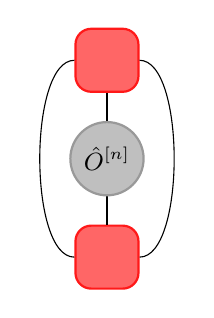
\begin{tikzpicture}[inner sep=1mm]
	\def \vdist {2.5}

	\node[tensorc] (tens1) at (1,0) {};
	\node[tensorc] (tens2) at (1,-\vdist) {}; 
	
	\draw[-] (tens1) -- (tens2);	
	
 	\node[operator] (op) at (1,-\vdist/2) {\small $\hat{O}^{[n]}$};
 	
 
    \draw[-] (tens1.west) .. controls (0, 0) and (0, -\vdist) .. (tens2.west);
    \draw[-] (tens1.east) .. controls (2, 0) and (2, -\vdist) .. (tens2.east);
\end{tikzpicture}
	\label{fig:SingleSiteOperator}
\end{subfigure}
\begin{subfigure}[b]{0.35\textwidth}
	\caption{}    
  	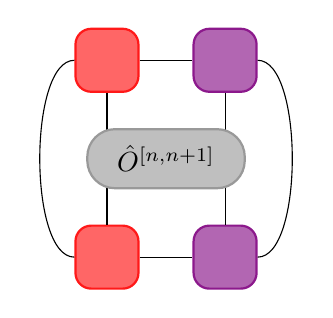
\begin{tikzpicture}[inner sep=1mm]
	\def \vdist {2.5}
	\def \hdist {1.5}
	\def \wid {2}

	\node[tensorc] (tens1) at (1,0) {};
	\node[tensorc] (tens2) at (1,-\vdist) {};
	\node[tensorr] (tens3) at (1 + \hdist,0) {};
	\node[tensorr] (tens4) at (1 + \hdist,-\vdist) {};

	\draw[-] (tens1) -- (tens2);
 	\draw[-] (tens3) -- (tens4);
 	\draw[-] (tens1) -- (tens3);
 	\draw[-] (tens2) -- (tens4);
	 
 	\node[twositeop, minimum width= \wid cm] (op) at (1 + \hdist/2 ,-\vdist/2) { $\hat{O}^{[n, n+1]}$};
 	
 
    \draw[-] (tens1.west) .. controls (0, 0) and (0, -\vdist) .. (tens2.west);
    \draw[-] (tens3.east) .. controls (2+\hdist, 0) and (2+\hdist, -\vdist) .. (tens4.east);
\end{tikzpicture}
	\label{fig:DoubleSiteOperator}
\end{subfigure}
\caption{\textit{Measurement of local properties of a matrix product state in the mixed-canonical form.}}
\end{figure}
Very similar is the case of multiple-site local operator. However, sites on which the operator act can not be contracted explicitly. Thus, the resulting tensor network will look like the example shown in figure \ref{fig:DoubleSiteOperator}, where a two-site operator is measured.\\

Correlation functions can also be calculated efficiently using matrix product states in the mixed-canonical form. Consider the correlation $\bra{\psi} \hat{O}^{[n]} \hat{Q}^{[n+k]} \ket{\psi}$, whose corresponding tensor network is shown in figure \ref{fig:CorrelationFunction}.
\begin{figure}[h!]
	\centering
	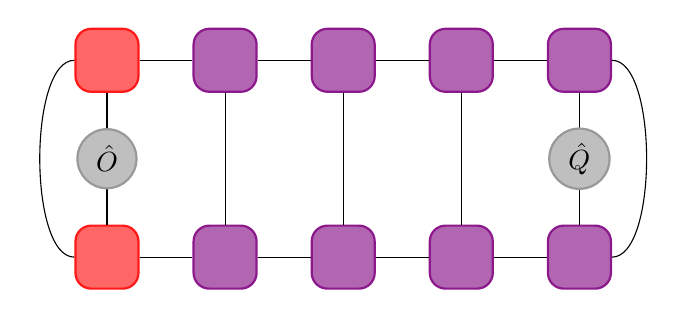
\begin{tikzpicture}[inner sep=1mm]
	\def \vdist {2.5};
	\def \hdist {1.5};
	\def \wid {2};
	\def \numb {5};

	\node[tensorc] (tt1) at (1*\hdist,0) {};
	\node[tensorc] (tb1) at (1*\hdist,-\vdist) {};
	
	 \foreach \i in {2,...,\numb} {
        \node[tensorr] (tt\i) at (\i*\hdist, 0) {};
		\node[tensorr] (tb\i) at (\i*\hdist,-\vdist) {};
           
        \draw[-] (tt\i) -- (tb\i);
    };
    
    \foreach \i in {2,...,4} {
        \pgfmathtruncatemacro{\iplusone}{\i + 1};
        \draw[-] (tt\i) -- (tt\iplusone);
        \draw[-] (tb\i) -- (tb\iplusone);
	};

	\draw[-] (tt1) -- (tb1);
 	\draw[-] (tt1) -- (tt2);
 	\draw[-] (tb1) -- (tb2);
 	 
 	\node[operator] (op1) at (1*\hdist,-\vdist/2) {$\hat{O}$};
	\node[operator] (op2) at (\numb*\hdist,-\vdist/2) { $\hat{Q}$};
  
 
    \draw[-] (tt1.west) .. controls (\hdist-1, 0) and (\hdist-1, -\vdist) .. (tb1.west);
    \draw[-] (tt\numb.east) .. controls (1+\numb*\hdist, 0) and (1+\numb*\hdist, -\vdist) .. (tb\numb.east);
\end{tikzpicture}
	\caption{\textit{Tensor network for the correlation function $\bra{\psi} \hat{O}^{[n]} \hat{Q}^{[n+4]} \ket{\psi}$. The outer parts of the network are implicitly contracted to identities following the mixed-canonical form of the MPS.}}
	\label{fig:CorrelationFunction}
\end{figure}
Bringing the MPS into a mixed-canonical form with the central tensor at site $m$ results in the outer parts of the network being explicitly contracted as identities. However, the otherwise right-normalized tensors between the two operators can not be contracted as identities, as the right-most operator breaks the canonical form. Thus, one has to contract a network of length $k+1$, which is done most efficiently following the optimal bracketing described in eq. \eqref{eq:optBracketsMPO}. The complexity of the entire contraction is of order $O(k D^3 d)$.

\subsection{Correlation length} \label{sec:CorrelationLength}
Although the MPS formalism excels at describing one dimensional systems, it struggles with describing long ranged correlations, due to how it is constructed.
Consider a general MPS in no particular canonical form, as described in eq. \eqref{eq:generalMPS}. The \textit{transfer operator} is defined as
\begin{equation}
	\hat{E}^{[n]} = \sum_{\alpha_{n-1}, \alpha_{n-1}'} \sum_{\alpha_{n}, \alpha_{n}'} E_{(\alpha_{n-1} \alpha_{n-1}'),(\alpha_{n}  \alpha_{n}')}^{[n]} \left( \ket{\alpha_{n-1}}\bra{\alpha_{n-1}'} \right) \left( \ket{\alpha_{n}}\bra{\alpha_{n}'} \right) \; ,
\end{equation}   
where $E^{[n]}$ are the matrix elements of the transfer operator
\begin{equation}
	E^{[n]} = \sum_{j_n} M^{[n] j_n *} \otimes M^{[n] j_n}  \; . \label{eq:transfermatrixelem1}
\end{equation}
The transfer operator is essentially a complete, positive map from operators defined on a block of the lattice of length $n-1$ to a block of length $n$, such that
\begin{equation}
	\{ \ket{\alpha_{n-1}}\bra{\alpha_{n-1}'} \} \to \{ \ket{\alpha_{n}}\bra{\alpha_{n}'} \} \; .
\end{equation}
The most important property of the transfer matrix is that all its eigenvalues $|\lambda_k| \leq 1 $ if the corresponding state is either left- or right-normalized \cite{schollwock}. \\
Generalizing the transfer operator matrix elements \eqref{eq:transfermatrixelem1} to contraction with an operator $\hat{O}$ at site $n$ yields 
\begin{equation}
	E_{O}^{[n]} = \sum_{j_n , j_n '} O^{j_n , j_n '} M^{[n] j_n *} \otimes  M^{[n] j_n '} \; . \label{eq:transfermatrixelem2}
\end{equation}
Thereby, correlation functions can be expressed using only the transfer matrices of eq. \eqref{eq:transfermatrixelem1} and \eqref{eq:transfermatrixelem2}. Assuming a translational invariant transfer matrices for a left-normalized state, whereby the correlation can be expressed as  
\begin{align}
	\bra{\psi} \hat{O}^{[i]} \hat{O}^{[j]} \ket{\psi} &= \Tr E^{[1]} \ldots E^{[i-1]} E_{O}^{[i]} E^{[i+1]} \ldots E^{[j-1]} E_{O}^{[j]} E^{[j+1]} \ldots E^{[L]} \nonumber \\
	&= \Tr E_{O}^{[i]} E^{j-i-1} E_{O}^{[j]} E^{L-j+i-1} \nonumber \\ 
	&= \sum_{l , k} \bra{l} E_{O}^{[i]} \ket{k} \lambda_{k}^{j-i-1} \bra{k} E_{O}^{[j]} \ket{l} \lambda_{l}^{L-j+i-1} \nonumber \\ 
	&= \sum_{k} \bra{1} E_{O}^{[i]} \ket{k} \lambda_{k}^{j-i-1} \bra{k} E_{O}^{[j]} \ket{1} \qquad (\mathrm{for } L \to \infty)
\end{align}
where $\ket{k}$ and $\ket{l}$ are eigenstates of the transfer operator with eigenvalues $\lambda$. Since $|\lambda_k| \leq 1 $, only the leading eigenvalue $\lambda_1 = 1$ remains as $L \to \infty$. Defining the distance between two sites as $r = |j - i -1|$ and the correlation  length as $\xi_k = -1/\ln \lambda_k$, the correlation function can be written as
\begin{equation}
	\frac{\bra{\psi} \hat{O}^{[i]} \hat{O}^{[j]} \ket{\psi}}{\braket{\psi | \psi}} = c_1 + \sum_{k = 2} c_k e^{-r/ \xi_k} \; , \label{eq:corrfunction}
\end{equation}
where $c_k = \bra{1} E_{O}^{[i]} \ket{k} \bra{k} E_{O}^{[j]} \ket{1}$. \cite{schollwock} \\
According to eq. \eqref{eq:corrfunction}, correlation functions are given by a linear combination of exponential functions in the MPS description. Therefore, matrix product states struggle describing long range correlations, such as the superfluid single-particle correlations. While single-particle correlations decay exponentially for the Mott-Insulator, it decays following a power-law for superfluids
\begin{equation}
	\braket{\hat{a}_{i}^{\dag} \hat{a}_{j}} \sim |i - j|^{-K_b /2} \; ,
	\label{eq:superfluidCorrelation}
\end{equation}
where $K_b$ is the Tomonaga-Luttinger parameter \cite{characPhases}. For short distances eq. \eqref{eq:corrfunction} is able to accurately approximate a power-law, however, only the slowest exponential decay will survive as distances grow larger. Hence, the correlation turns into a pure exponential decay with $\xi = -1/ \ln \lambda$, where $\lambda$ is the largest eigenvalue of $\hat{E}$ contributing to the correlation.\\
To demonstrate the correlation properties of matrix product states, consider figure \ref{fig:DensityMatrices}.
\begin{figure}[h!]
    \centering
    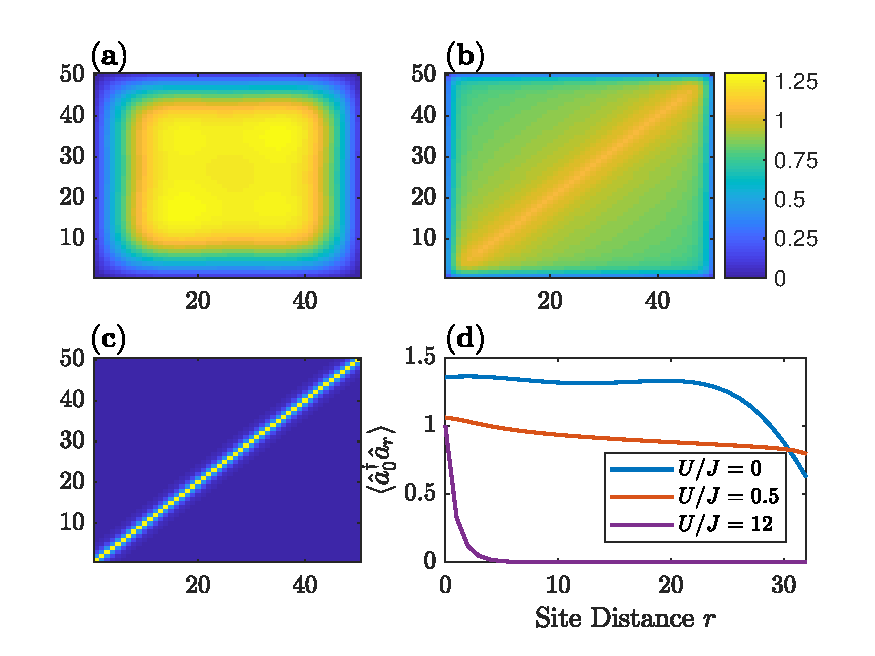
\includegraphics[width=0.8\textwidth]{Figures/DensityMatrices.pdf}
    \caption{\textit{\textbf{(a-c)} Density matrices of a 50 site system for $U/J = 0, \; 0.5, \; 12$. \textbf{d} entries of the 15th row of the density matrices plotted as a function of distance from the diagonal, $r$. }}
    \label{fig:DensityMatrices}
\end{figure}
The figure depict the density matrix with entries $\rho_{i,j} = \bra{\psi} \hat{a}_{i}^{\dag} \hat{a}_{j} \ket{\psi}$ for the ground state of a Bose-Hubbard system with $L = 50$ sites and unit occupancy. The ground state was found at various fractions of $U/J$ using the DMRG algorithm detailed in Section \ref{sec:DMRG}.
Figures \ref{fig:DensityMatrices}.a and \ref{fig:DensityMatrices}.c show the density matrix plotted for the superfluid and the Mott-Insulator limit respectively. In the superfluid limit, long-range correlations are present, which is seen by large off-diagonal elements. However, since all correlations decay exponentially in the MPS description, the algorithm has difficulty approximating the very long range correlations of the system. This is visualized in figure \ref{fig:DensityMatrices}.d, where the correlation function is plotted against distance from the diagonal. The superfluid graph has a hump on it, which is an artifact of the MPS description and DMRG algorithm. Due to the very long correlation length, the graph should be almost flat except for the rapid drop in the end, which is due to the closed boundary conditions.\\
In the Mott-Insulator limit no interaction takes place between sites, and the correlation length is zero. Hence, the correlation matrix contains only diagonal elements of equal magnitude. Figure \ref{fig:DensityMatrices}.c shows some off-diagonal elements of non-zero magnitude, since the system is not a pure Mott-Insulator at $U/J = 12$. Nevertheless, the correlations are well described by only a single exponential function, as seen by the figure.\\
Finally, figure \ref{fig:DensityMatrices}.ii illustrates the density matrix for a system with $U/J = 0.5$, which is primarily a superfluid. The particles are not completely de-localized, which is noticeable from the well defined diagonal. Plotting the correlation function reveals the best approximation being a power-law, confirming the system is indeed a superfluid. 

\chapter{Tensor Network Algorithms}
Although matrix product states enables analytical treatment of certain classes of quantum states \cite{Baxter1968,Affleck1987}, their real power becomes evident when performing numerical computations. These computations require algorithms capable of exploiting the properties of the matrix product states. The Density-Matrix Renormalization Group (DMRG) was developed as the most powerful numerical method to study one-dimensional quantum lattice systems \cite{White1992,White1993}. The DMRG algorithm is a variational ground state search method, which owes its effectiveness to the entanglement area law scaling of most ground states in one-dimensional lattice systems. Therefore, the DMRG method only has to search a tiny corner of the otherwise exponentially large Hilbert space \cite{Cramer}, which enables its application on systems much larger  than what is accessible through exact diagonalization.

Years later the connection between the DMRG method and matrix product states was made, as these two approaches share many features \cite{Ostlund1995, Dukelsky1998}. Formulating the DMRG method in the MPS language made several extensions to the algorithm possible, which would otherwise have been very difficult to express within the DMRG framework \cite{schollwock}. Among these extensions one finds the tDMRG algorithm \cite{Vidal2003,Vidal2004,Daley2004}, which borrows elements from DMRG in order to perform time-evolution of a matrix product state.
Due to the light-cone-like propagation of information within the quantum system \cite{Lauchli2008,Bravyi2006}, a state initially following an area law will continue to do so for longer times \cite{Bravyi2006,Eisert2006}, although the prefactor of the area law scales exponentially with the system size \cite{Schuch2008}. Therefore, tensor-network methods are capable of efficiently simulating out-of-equilibrium dynamics for short time-scales \cite{Eisert2015}.


\section{Variational Ground State Search}
For large systems exact diagonalization of the Hamiltonian is impossible, whereby one must resort to variational methods in order to find ground states. A variational search involves finding the state, $\ket{\psi}$, which minimizes
\begin{equation}
	E = \frac{\bra{\psi} \hat{H} \ket{\psi}}{\braket{\psi | \psi}} \; .
	\label{eq:variational}
\end{equation}
The Hamiltonian must be expressed as a matrix product operator to be applied to the state. An example is given in Appendix \ref{chap:buildMPO}, where the Bose-Hubbard Hamiltonian is formulated through tensors. Furthermore, in a variational search the state is repeatedly modified until the expectation value of the Hamiltonian is minimized. Therefore, the tensor network corresponding to eq. \ref{eq:variational} must be contracted efficiently in order for the search to be viable.


\subsection{Efficient Application of a Hamiltonian to an MPS}
Section \ref{sec:MPO} detailed the application of a matrix product operator to a state, however, even further reductions to the computational cost are needed, as the overlap with the Hamiltonian is evaluated many times during the ground state search. The DMRG variational search algorithm updates only a single tensor of the state at a time, whereby most of the tensor network describing the operator overlap remains constant. Hence, most of the network can be stored and used for multiple calculations, which is one of the key properties of the DMRG algorithm.\\ 
Consider a matrix product state in a mixed-canonical form
\begin{align}
	\ket{\psi} &= \sum_{\boldsymbol{j}} A^{j_1} \ldots A^{j_{n-1}} \Psi^{j_n} B^{j_{n+1}} \ldots B^{j_{L}} \ket{\boldsymbol{j}} \nonumber \\
	&= \sum_{\alpha_{n-1} , \alpha_{n}} \Psi_{\alpha_{n-1} , \alpha_{n}}^{j_n} \ket{\alpha_{n-1}}_A \ket{j_n}  \ket{\alpha_{n}}_L \; ,
	\label{eq:MPSmixedsingle}
\end{align}
where $\Psi^{j_n}$ are the matrices of the central site, and $\ket{\alpha_{n-1}}_A$ and $\ket{\alpha_{n}}_B$ are block states introduced in eq. \eqref{eq:mixedA} and \eqref{eq:mixedB} respectively. In the basis $\{ \ket{\alpha_{n-1} } \; , \; \ket{ j_n } \; , \; \ket{\alpha_{n} } \}$ the individual matrix elements of the Hamiltonian can be expressed as
\begin{equation*}
	\bra{\alpha_{n-1} j_n \alpha_{n}} \hat{H} \ket{\alpha_{n-1} ' j_n ' \alpha_{n} '} = \sum_{\boldsymbol{j} , \boldsymbol{j'}}  W^{j_1 , j_1 '} \ldots W^{j_L , j_L '}  \braket{\alpha_{n-1} j_n \alpha_{n} | \boldsymbol{j}} \braket{\boldsymbol{j'} | \alpha_{n-1} ' j_n ' \alpha_{n} '} \; . 
\end{equation*}
Since the basis of local states $\{ \ket{\boldsymbol{j}} \}$ shares a state with the basis $\{ \ket{\alpha_{n-1} } \; , \; \ket{ j_n } \; , \; \ket{\alpha_{n} } \}$, the above expression can be re-written using $\sum_{\boldsymbol{j}} \braket{j_n | \boldsymbol{j}} = \sum_{\boldsymbol{j *}} \ket{ \boldsymbol{j *}}$, where "$\boldsymbol{*}$" means "excluding $j_n$". Thus,
\begin{align}
&	\bra{\alpha_{n-1} j_n \alpha_{n}} \hat{H} \ket{\alpha_{n-1} ' j_n ' \alpha_{n} '} = \nonumber \\
 &= \sum_{\boldsymbol{j *} , \boldsymbol{j' * }}  W^{j_1 , j_1 '} \ldots W^{j_n , j_n '} \ldots W^{j_L , j_L '} \nonumber \\
	& \qquad \times \braket{\alpha_{n-1} | j_1 \ldots j_{n-1}} \braket{\alpha_{n} | j_{n+1} \ldots j_{L}} \braket{j_1 ' \ldots j_{n-1} ' | \alpha_{n-1} '} \braket{j_{n+1} ' \ldots j_{L} ' | \alpha_{n} '} \nonumber \\
	&= \sum_{\boldsymbol{j *} , \boldsymbol{j' * }}  W^{j_1 , j_1 '} \ldots W^{j_n , j_n '} \ldots W^{j_L , j_L '} \nonumber \\
	& \qquad \times \left( A^{j_1} \ldots A^{j_{n-1}} \right)_{1 , \alpha_{n-1}}^{*} \left( B^{j_{n+1}} \ldots B^{j_{L}} \right)_{ \alpha_{n} , 1}^{*} \left( A^{j_1 '} \ldots A^{j_{n-1} '} \right)_{1 , \alpha_{n-1} '} \left( B^{j_{n+1} '} \ldots B^{j_{L} '} \right)_{ \alpha_{n} ' , 1} \nonumber \\
	&= \sum_{\alpha_n , \beta_n , \alpha_n '}
	\left( \sum_{j_1 , j_1 '} A_{1 , \alpha_1}^{j_1 *} W_{1, \beta_1}^{j_1 , j_1 '} A_{1 , \alpha_1 '}^{j_1 '} \right)
	\left( \sum_{j_2 , j_2 '} A_{\alpha_1 , \alpha_2}^{j_2 *} W_{\beta_1, \beta_2}^{j_2 , j_2 '} A_{\alpha_1 ' , \alpha_2 '}^{j_2 '} \right)
	\ldots W_{\beta_{n_1}, \beta_n}^{j_n , j_n '} \nonumber \\
	& \qquad \times \left( \sum_{j_{n+1} , j_{n+1} '} B_{\alpha_n , \alpha_{n+1}}^{j_{n+1} *} W_{\beta_n, \beta_{n+1}}^{j_{n+1} , j_{n+1} '} B_{\alpha_n ', \alpha_{n+1} '}^{j_{n+1} '} \right)
	\left( \sum_{j_{L} , j_{L} '} B_{\alpha_{L-1} , 1}^{j_{L} *} W_{\beta_{L-1}, 1}^{j_{L} , j_{L} '} B_{\alpha_{L-1}' , 1 }^{j_{L} '} \right)  \; .
\end{align}  
While this expression may seem terrible complicated due to all the indices, it is actually rather easy to understand. First, the matrix element is written excluding the local basis states $\ket{j_n}$. Next, the Hamilton MPO is projected into the block states of A, $\ket{\alpha_{n-1}}_A$, and B, $\ket{\alpha_{n}}_B$. Finally, the matrices are grouped according to their expansion in the local basis. Working with the above expression appears cumbersome, but it is merely a decoupling of the system into three distinct parts, which can be seen in figure \ref{fig:singleElemHamil}.
\begin{figure}[h!]
	\centering
	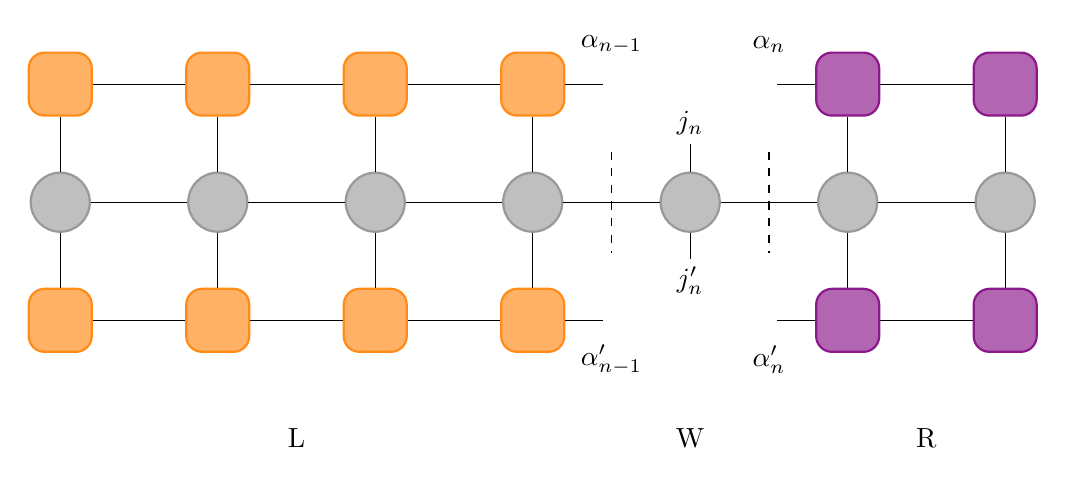
\begin{tikzpicture}[inner sep=1mm]
    \foreach \i in {1,...,4} {
        \node[tensorl] (tt\i) at (2* \i -1, 0) {};
        \node[operator] (o\i) at (2* \i -1, -1.5) {};
        \node[tensorl] (tb\i) at (2* \i -1, -3) {};
        
        
        \draw[-] (tt\i) -- (o\i);
        \draw[-] (o\i) -- (tb\i);
    };
    \foreach \i in {6,...,7} {
        \node[tensorr] (tt\i) at (2* \i -1, 0) {};
        \node[operator] (o\i) at (2* \i -1, -1.5) {};
        \node[tensorr] (tb\i) at (2* \i -1, -3) {};
        
        
        \draw[-] (tt\i) -- (o\i);
        \draw[-] (o\i) -- (tb\i);
    };
        \foreach \i in {1,...,3} {
        \pgfmathtruncatemacro{\iplusone}{\i + 1};
        \draw[-] (tt\i) -- (tt\iplusone);
        \draw[-] (tb\i) -- (tb\iplusone);
        \draw[-] (o\i) -- (o\iplusone);
    };
    \draw[-] (tt6) -- (tt7);
    \draw[-] (tb6) -- (tb7);
    \draw[-] (o6) -- (o7);
    
    
       
	\node[operator] (o5) at (2* 5 -1, -1.5) {};    
    
    \node (a1) at (8,0.5) {$\alpha_{n-1}$};
    \node (a2) at (10,0.5) {$\alpha_{n}$};
    \node (a1p) at (8,-3.5) {$\alpha_{n-1} '$};
    \node (a2p) at (10,-3.5) {$\alpha_{n} '$};
    \node (j) at (9,-0.5) {$j_n$};
    \node (jp) at (9,-2.5) {$j_n '$};
    
    \node (a1d) at (8,0) {};
    \node (a2d) at (10,0) {};
    \node (a1pd) at (8,-3) {};
    \node (a2pd) at (10,-3) {};
    
    \draw[-] (tt4) -- (a1d);
    \draw[-] (tt6) -- (a2d);
    \draw[-] (tb4) -- (a1pd);
    \draw[-] (tb6) -- (a2pd);
    \draw[-] (o5) -- (j);
    \draw[-] (o5) -- (jp);
    \draw[-] (o5) -- (o4);
    \draw[-] (o5) -- (o6);
    
    \node (d1) at (8,-0.75) {};
    \node (d2) at (8,-2.25) {};
   	\draw[dashed] (d1) -- (d2);
   	\node (d3) at (10,-0.75) {};
    \node (d4) at (10,-2.25) {};
   	\draw[dashed] (d3) -- (d4);
   	
   	
   	\node (L) at (4,-4.5) {L};
   	\node (W) at (9,-4.5) {W};
   	\node (R) at (12,-4.5) {R};
\end{tikzpicture}
	\caption{Representation of the matrix element $\bra{\alpha_{n-1} j_n \alpha_{n}} \hat{H} \ket{\alpha_{n-1} ' j_n ' \alpha_{n} '}$ as an tensor network. The network can be factorize into three distinct parts: The left (L) and right (R) environments consisting of the contracted network to the left and right of the operator tensor, $W^{[n]}$, respectively.}
	\label{fig:singleElemHamil}
\end{figure}
Since both the left and right side of the network is connected, one can contract these parts into two separate tensors $L$ and $R$ called \textit{environments}:
\begin{align}
	L_{\alpha_{n}, \beta_{n} , \alpha_{n} '} &= \sum_{ \substack{ \{ \alpha_i \beta_i \alpha_i ' \} \\ i < n}} \left( \sum_{j_1 , j_1 '} A_{1 , \alpha_1}^{j_1 *} W_{1, \beta_1}^{j_1 , j_1 '} A_{1 , \alpha_1 '}^{j_1 '} \right) \ldots \left( \sum_{j_{n} , j_{n} '} A_{\alpha_{n-1} , \alpha_{n}}^{j_{n} *} W_{\beta_{n-1}, \beta_{n}}^{j_{n} , j_{n} '} A_{\alpha_{n-1} ' , \alpha_{n} '}^{j_{n} '} \right) \label{eq:Ltensor} \\
	R_{\alpha_{n} ,\beta_{n} , \alpha_{n} '} &= \sum_{ \substack{ \{ \alpha_i \beta_i \alpha_i ' \} \\ i > n}} \left( \sum_{j_{n+1}  j_{n+1} '} B_{\alpha_n , \alpha_{n+1}}^{j_{n+1} *} W_{\beta_n, \beta_{n+1}}^{j_{n+1} , j_{n+1} '} B_{\alpha_n ', \alpha_{n+1} '}^{j_{n+1} '} \right) \ldots \nonumber \\
	& \qquad \qquad \qquad \qquad \qquad \qquad \qquad \times \left( \sum_{j_{L} , j_{L} '} B_{\alpha_{L-1} , 1}^{j_{L} *} W_{\beta_{L-1}, 1}^{j_{L} , j_{L} '} B_{\alpha_{L-1}' , 1 }^{j_{L} '} \right) \label{eq:Rtensor}
\end{align}
From these contractions, the tripartite structure of the Hamiltonian matrix elements, as seen in figure \ref{fig:singleElemHamil}, can be written in a compact way
\begin{equation}
	\bra{\alpha_{n-1} j_n \alpha_{n}} \hat{H} \ket{\alpha_{n-1} ' j_n ' \alpha_{n} '} = \sum_{\beta_{n-1} , \beta_{n}} L_{\alpha_{n-1}, \beta_{n-1} , \alpha_{n-1} '} \; W_{\beta_{n_1}, \beta_n}^{j_n , j_n '} \; R_{\alpha_{n} ,\beta_{n} , \alpha_{n} '} \; .
\end{equation}
Finally, applying the Hamiltonian in the $\{ \ket{\alpha_{n-1} } \; , \; \ket{ j_n } \; , \; \ket{\alpha_{n} } \}$ basis to the MPS of eq. \eqref{eq:MPSmixedsingle} yields \cite{schollwock}
\begin{equation}
	\hat{H} \ket{\psi} = \sum_{\beta_{n-1} , \beta_{n}} \sum_{\alpha_{n-1}' , j_n ', \alpha_{n}'} L_{\alpha_{n-1}, \beta_{n-1} , \alpha_{n-1} '} \; W_{\beta_{n_1}, \beta_n}^{j_n , j_n '} \; R_{\alpha_{n} ,\beta_{n} , \alpha_{n} '} \; \Psi_{\alpha_{n-1} ' , \alpha_{n} '}^{j_n '} \ket{\alpha_{n-1}}_A \ket{j_n} \ket{\alpha_{n}}_B \; .
	\label{eq:HPsi}
\end{equation}
Expressing $\hat{H}$ in the basis of the block states exposes the central site of the MPS such that it can be varied in a ground state search. Evaluating $\hat{H} \ket{\psi}$ must be done many times during a variational search of the ground state, hence this operation must be executed as fast as possible. Examining eq. \eqref{eq:HPsi} one will notice that while the boundaries of $L$ and $R$ will change depending on which site is being optimized, the bulk of the two tensors remain constant through most of the calculations. Instead of calculating $L$ and $R$ from eq. \eqref{eq:Ltensor} and \eqref{eq:Rtensor} for every evaluation of eq. \eqref{eq:HPsi}, one can iteratively build them, since they only change by one column of the network at a time. Thus, a large number of computations can be reused.\\
Consider the construction of the tensor $L^{[i]}$, which can be built iteratively from the left by contracting the previous left-tensor $L^{[i-1]}$ with the i'th column of the network consisting of $A^{[i]}$, $W^{[i]}$ and $A^{[i] \dag}$
\begin{equation}
	L_{\alpha_i , \beta_i , \alpha_i '}^{[i]} = \sum_{\substack{ j_i , j_i ' \\ \alpha_{i-1} , \beta_{i-1} , \alpha_{i-1} '}} W_{\beta_{i-1} , \beta_i}^{[i] j_i , j_i '} \left( A^{[i] j_i \dag} \right)_{\alpha_i , \alpha_{i-1}} L_{\alpha_{i-1} , \beta_{i-1} , \alpha_{i-1} '}^{[i-1]} A_{\alpha_{i-1} ' , \alpha_i '}^{[i] j_i '} \; .
\end{equation}
The iterative update of $L^{[i]}$ can be seen illustrated in figure \ref{fig:buildLTensor}. The square-bracket notation has been re-introduced to keep track of the tensors relation to the physical sites. In order to remain consistent with notation, the dummy scalars $L_{\alpha_0 , \beta_0 , \alpha_0 '}^{[0]}  = 1  = \alpha_0 , \beta_0 , \alpha_0 '$ have been introduced.\\
\begin{figure}[h!]
	\centering
	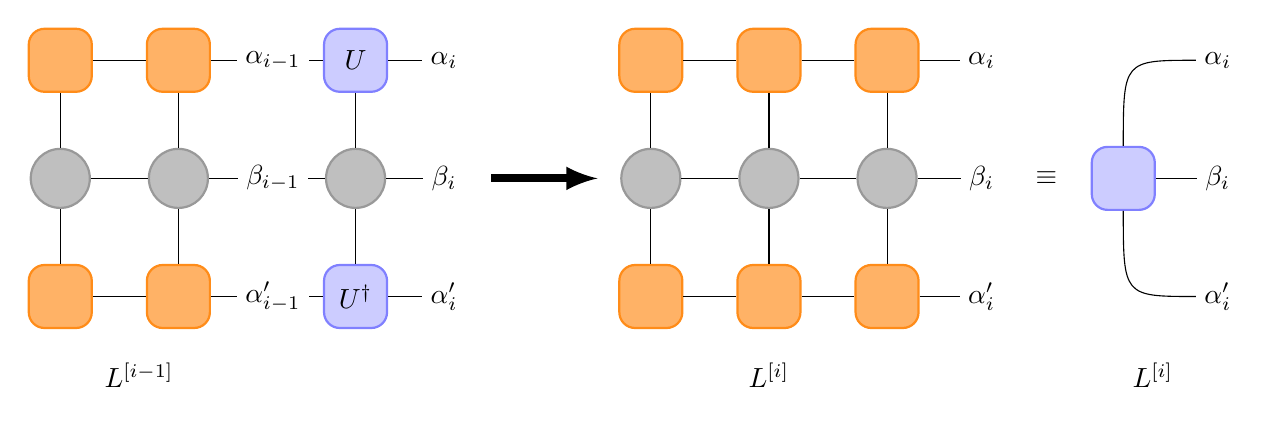
\begin{tikzpicture}[inner sep=1mm]
	\def \numb {2};
	\def \hdist {1.5};
	\def \offset {6};

    \foreach \i in {1,...,\numb} {
        \node[tensorl] (tt\i) at (\i*\hdist, 0) {};
        \node[operator] (o\i) at (\i*\hdist, -1.5) {};
        \node[tensorl] (tb\i) at (\i*\hdist, -3) {};  
        
        \draw[-] (tt\i) -- (o\i);
        \draw[-] (o\i) -- (tb\i);
    };
    \foreach \i in {1,...,1} {
        \pgfmathtruncatemacro{\iplusone}{\i + 1};
        \draw[-] (tt\i) -- (tt\iplusone);
        \draw[-] (tb\i) -- (tb\iplusone);
        \draw[-] (o\i) -- (o\iplusone);
    };
    \foreach \i in {\offset,...,8} {
        \node[tensorl] (tt\i) at (\i*\hdist, 0) {};
        \node[operator] (o\i) at (\i*\hdist, -1.5) {};
        \node[tensorl] (tb\i) at (\i*\hdist, -3) {};  
        
        \draw[-] (tt\i) -- (o\i);
        \draw[-] (o\i) -- (tb\i);
    };
    \foreach \i in {\offset,...,7} {
        \pgfmathtruncatemacro{\iplusone}{\i + 1};
        \draw[-] (tt\i) -- (tt\iplusone);
        \draw[-] (tb\i) -- (tb\iplusone);
        \draw[-] (o\i) -- (o\iplusone);
    };
    
    \node[tensor] (tt) at (\numb*\hdist+1.5*\hdist, 0) {$U$};
    \node[operator] (o) at (\numb*\hdist+1.5*\hdist, -1.5) {};
    \node[tensor] (tb) at (\numb*\hdist+1.5*\hdist, -3) {$U^{\dag}$};

	\draw[-] (tt) -- (o);
	\draw[-] (tb) -- (o);
    
    \node (at1) at (\numb*\hdist+0.8*\hdist, 0) {$\alpha_{i-1}$};
    \node (at2) at (\numb*\hdist+2.25*\hdist, 0) {$\alpha_{i}$};
    \node (ab1) at (\numb*\hdist+0.8*\hdist, -3) {$\alpha_{i-1} '$};
    \node (ab2) at (\numb*\hdist+2.25*\hdist, -3) {$\alpha_{i} '$};
    \node (b1) at (\numb*\hdist+0.8*\hdist, -1.5) {$\beta_{i-1}$};
    \node (b2) at (\numb*\hdist+2.25*\hdist, -1.5) {$\beta_{i}$};
    
    \draw[-] (tt\numb) -- (at1);
    \draw[-] (tb\numb) -- (ab1);
    \draw[-] (o\numb) -- (b1);
    \draw[-] (tt) -- (at1);
    \draw[-] (tb) -- (ab1);
    \draw[-] (o) -- (b1);
    \draw[-] (tt) -- (at2);
    \draw[-] (tb) -- (ab2);
    \draw[-] (o) -- (b2);
    
    
    \draw[->, line width=1mm] (\numb*\hdist+2.65*\hdist,-1.5) -- (\numb*\hdist+3.55*\hdist,-1.5);
    
    \node (at3) at (\offset*\hdist+\numb*\hdist+0.8*\hdist, 0) {$\alpha_{i}$};
    \node (ab3) at (\offset*\hdist+\numb*\hdist+0.8*\hdist, -3) {$\alpha_{i} '$};
    \node (b3) at (\offset*\hdist+\numb*\hdist+0.8*\hdist, -1.5) {$\beta_{i}$};
    \draw[-] (tt8) -- (at3);
    \draw[-] (tb8) -- (ab3);
    \draw[-] (o8) -- (b3);
    
    \node (L1) at (2.5,-4) {$L^{[i-1]}$};
    \node (L2) at (\offset*\hdist+\hdist,-4) {$L^{[i]}$};

    
    \node (eq) at (\offset*\hdist+\numb*\hdist+1.35*\hdist,-1.5) {$\equiv$};
    

    \node (dummy1) at (\offset*\hdist+\numb*\hdist+2.8*\hdist,0) {$\alpha_{i}$};
 	\node (dummy2) at (\offset*\hdist+\numb*\hdist+2.8*\hdist,-3) {$\alpha_{i} '$};
 	\node (dummy3) at (\offset*\hdist+\numb*\hdist+2.8*\hdist,-1.5) {$\beta_{i}$};
	\node[tensor] (mat) at (\offset*\hdist+\numb*\hdist+2*\hdist , -1.5) {};    
    
    \draw[-] (dummy1.west) .. controls (\offset*\hdist+\numb*\hdist+2*\hdist, 0) .. (mat.north);
    \draw[-] (dummy2.west) .. controls (\offset*\hdist+\numb*\hdist+2*\hdist, -3) .. (mat.south);
	\draw[-] (mat) -- (dummy3);   
	
	
	\node (L3) at (\offset*\hdist+\numb*\hdist+2.25*\hdist,-4) {$L^{[i]}$}; 
\end{tikzpicture}
	\caption{\textit{Iterative update from $L^{[i-1]}$ to $L^{[i]}$ through a contraction of $L^{[i-1]}$ with $A^{[i]}$, $W^{[i]}$ and $A^{[i] \dag}$. The result is a tensor with three horizontal legs.}}
	\label{fig:buildLTensor}
\end{figure}
It is important to store every iteration of $L^{[i]}$, since $L$ will grow and shrink constantly throughout the variational search of the ground state, whereby every iteration of $L^{[i]}$ will be used multiple times.
The same applies when building the right environment, $R$. Here one starts from the right and moves left when iteratively contracting the tensor. By applying optimal bracketing, the computational cost of updating the environments scales as $\mathcal{O}(d D^3 D_W)$.
  

\subsection{Iterative Ground State Search and the DMRG Algorithm} \label{sec:DMRG}
In order to find the ground state of the system on can introduce a Lagrangian multiplier, $\lambda$, and extremize
\begin{equation}
	\bra{\psi} \hat{H} \ket{\psi} - \lambda \braket{\psi | \psi} \; ,
	\label{eq:lagrange}
\end{equation}
whereby the desired ground state, $\ket{\psi}$, and ground state energy, $\lambda^0$, will be reached.\\
Trying to optimize an entire MPS at once is a highly non-linear problem involving an extremely large number of variables. However, the problem can be linearised by only considering the variables of a single tensor (site) at a time, while keeping the rest of the MPS constant. By varying just a single tensor at a time, one will continuously find states lower in energy, until convergence is reached. However, this procedure is very prone to getting stuck in a local extrema. To circumvent this, one can consider two sites at a time and optimize with regards to a two-site tensor, created by momentarily merging the two sites \cite{White1993}.

Consider the variation of the tensors $M^{[n]}$ and $M^{[n+1]}$. Expressing the minimization problem of eq. \eqref{eq:lagrange} in terms of the left and right environments (as done in eq. \eqref{eq:HPsi}) yields
\begin{align}
	\bra{\psi} \hat{H} \ket{\psi} &= \sum_{\substack{j_n , j_n ' \\ j_{n+1} , j_{n+1} '}} \sum_{\alpha_{n-1} ' , \alpha_n ', \alpha_{n+1} '} \sum_{\alpha_{n-1} , \alpha_n , \alpha_{n+1}} \sum_{\beta_{n-1} , \beta_n , \beta_{n+1}} L_{\alpha_{n-1}, \beta_{n-1} , \alpha_{n-1} '}^{[n-1]} \; W_{\beta_{n_1}, \beta_n}^{j_n , j_n '} \; W_{\beta_{n}, \beta_{n+1}}^{ j_{n+1} , j_{n+1} '} \nonumber \\
	& \qquad \times R_{\alpha_{n+1} ,\beta_{n+1} , \alpha_{n+1} '}^{[n+2]} \; M_{\alpha_{n-1} , \alpha_{n}}^{j_n } \; M_{\alpha_{n-1} ' , \alpha_{n} '}^{j_n ' *} \; M_{\alpha_{n} , \alpha_{n+1}}^{j_{n+1} } \; M_{\alpha_{n} ' , \alpha_{n+1} '}^{j_{n+1} ' *}  \label{eq:twositeHamil}
\end{align}
with the overlap
\begin{align}
	\braket{\psi | \psi} &= \sum_{j_n , j_{n+1} } \sum_{\substack{\alpha_{n-1} ' \\ \alpha_n ', \alpha_{n+1} '}} \sum_{\alpha_{n-1} , \alpha_n ,\alpha_{n+1}} \Psi_{\alpha_{n-1},\alpha_{n-1}'}^{A} \; M_{\alpha_{n-1} , \alpha_{n}}^{ j_n } \; M_{\alpha_{n-1} ' , \alpha_{n} '}^{j_n ' *} \nonumber \\
	& \qquad \times M_{\alpha_{n} , \alpha_{n+1}}^{j_{n+1} } \; M_{\alpha_{n} ' , \alpha_{n+1} '}^{j_{n+1} ' *} \; \Psi_{\alpha_{n+1},\alpha_{n+1}'}^{B} \; , \label{eq:twositeOverlap}
\end{align}
where the Hamiltonian from eq. \eqref{eq:HPsi} has been re-ordered to accommodate examining two sites, $n$ and $n+1$, at a time, and 
\begin{align}
\Psi_{\alpha_{n-1},\alpha_{n-1}'}^{A} &= \sum_{j_1 , \ldots , j_{n-1}} \left( M^{j_{n-1} \dag} \ldots M^{j_{1} \dag} M^{j_1} \ldots M^{j_{n-1}} \right) _{\alpha_{n-1} , \alpha_{n-1} '} \label{eq:psiA} \\
\Psi_{\alpha_{n+1},\alpha_{n+1}'}^{B} &= \sum_{j_{n+2} , \ldots , j_{L}} \left( M^{j_{n+2} } \ldots M^{j_{L} } M^{j_L \dag} \ldots M^{j_{n+2} \dag} \right) _{\alpha_{n+1} ', \alpha_{n+1} } \; .
\end{align}
Further simplifications can be made for mixed-canonical forms, if sites $1$ through $n-1$ are left-normalized, and sites $n+2$ through $L$ are right-normalized, whereby
\begin{equation}
	\Psi_{\alpha_{n-1},\alpha_{n-1}'}^{A} = \delta_{\alpha_{n-1},\alpha_{n-1}'} \qquad , \qquad \Psi_{\alpha_{n+1},\alpha_{n+1}'}^{B} = \delta_{\alpha_{n+1},\alpha_{n+1}'} \; .
\end{equation}
Finding the extremum of eq. \eqref{eq:lagrange} with respect to $M_{\alpha_{n-1} ' , \alpha_{n} '}^{[n] j_n ' } \; M_{\alpha_{n} ' , \alpha_{n+1} '}^{[n+1] j_{n+1} ' }$ is done through the following sequence:

\subsubsection{Two-site update for iterative ground state search}
\begin{enumerate}
\item
\textbf{Merge:} Contract the two matrices $M^{[n]}$ and $M^{[n+1]}$ over the bond $\alpha_{n}$ creating a two-site tensor
\begin{equation}
\Theta_{\alpha_{n-1} , \alpha_{n+1}}^{j_n , j_{n+1}} = \sum_{\alpha_n} M_{\alpha_{n-1} , \alpha_{n}}^{[n] j_n } \;  M_{\alpha_{n} , \alpha_{n+1}}^{[n+1] j_{n+1} } 
\end{equation}

\item
\textbf{Solve eigenproblem:} This yields an eigenvalue problem, which can be seen by reshaping
\begin{align}
	H_{( \alpha_{n-1}  j_n  j_{n+1}, \alpha_{n+1}),(\alpha_{n-1}'  j_n '  j_{n+1}', \alpha_{n+1}')} &= \nonumber \\
	= \; \sum_{\substack{\beta_{n-1} , \beta_n \\ \beta_{n+1}}} L_{\alpha_{n-1}, \beta_{n-1} , \alpha_{n-1} '}^{[n-1]} & \; W_{\beta_{n_1}, \beta_n}^{[n] j_n , j_n '} \; W_{\beta_{n}, \beta_{n+1}}^{[n+1] j_{n+1} , j_{n+1} '}\;  R_{\alpha_{n+1} ,\beta_{n+1} , \alpha_{n+1} '}^{[n+2]} 
\end{align}
and
\begin{equation}
	v_{ \alpha_{n-1} j_n j_{n+1} \alpha_{n+1}} = \; \Theta_{\alpha_{n-1} , \alpha_{n+1}}^{j_n , j_{n+1}}
\end{equation}
such that
\begin{equation}
	H v - \lambda v = 0 \; .
	\label{eq:eigprob}
\end{equation}
Solving eq. \eqref{eq:eigprob} for the lowest eigenvalue $\lambda_0$ yields $v_{ \alpha_{n-1} j_n j_{n+1} \alpha_{n+1}}^0$, which can be reshaped back to the now optimized two-site tensor, $\tilde{\Theta}_{\alpha_{n-1} , \alpha_{n+1}}^{j_n , j_{n+1}}$.

\item
\textbf{Unmerge:} Reshape the updated $\tilde{\Theta}_{\alpha_{n-1} , \alpha_{n+1}}^{j_n , j_{n+1}}$ to a matrix and perform an SVD yielding
\begin{equation}
	\tilde{\Theta}_{(j_n \alpha_{n-1} ) ,(j_{n+1}  \alpha_{n+1} )} = \sum_{\alpha_n} U_{\alpha_{n-1} , \alpha_{n}}^{j_n} S_{\alpha_n , \alpha_n} (V^{\dag})_{\alpha_{n} , \alpha_{n+1}}^{j_{n+1}} \; .
\end{equation}
This causes the bond dimension to increase $D \rightarrow d D$, which must be truncated by keeping only the $D$ largest singular values of $S$. 

\item
\textbf{Update environments:} The last step depends on which direction, one is iterating trough the chain. Here, the left- and right-normalization of $U$ and $V^{\dag}$ is used to update the environments.\\
\textit{Going right}: Update the left environment
\begin{equation}
	\tilde{L}_{\alpha_{n}, \beta_{n} , \alpha_{n} '}^{[n]} = \sum_{\substack{ j_{n} , j_{n} ' \\ \alpha_{n-1} , \beta_{n-1} , \alpha_{n-1} '}} L_{\alpha_{n-1}, \beta_{n-1} , \alpha_{n-1} '}^{[n-1]} \; U_{\alpha_{n-1} , \alpha_{n}}^{j_n} \; W_{\beta_{n-1} , \beta_{n}}^{[n] j_n , j_n '} \; U_{\alpha_{n-1} ', \alpha_{n}'}^{j_n ' *} \; ,
\label{eq:updateLeft}
\end{equation}
and build the matrix of the right site
\begin{equation}
	\tilde{M}_{\alpha_{n} , \alpha_{n+1}}^{[n+1] j_{n+1} } = \sum_{\alpha_n}  S_{\alpha_n , \alpha_n} (V^{\dag})_{\alpha_{n} , \alpha_{n+1}}^{j_{n+1}} \; .
\end{equation}\\ 
\textit{Going left}: Update the right environment
\begin{equation}
	\tilde{R}_{\alpha_{n}, \beta_{n} , \alpha_{n} '}^{[n+1]} = \sum_{\substack{ j_{n+1} , j_{n+1} ' \\ \alpha_{n+1} , \beta_{n+1} , \alpha_{n+1} '}} R_{\alpha_{n+1}, \beta_{n+1} , \alpha_{n+1} '}^{[n+2]} \; \left( V^{\dag} \right)_{\alpha_{n} , \alpha_{n+1}}^{j_{n+1}} \; W_{\beta_{n} , \beta_{n+1}}^{[n+1] j_{n+1} , j_{n+1} '} \; \left( V^{\dag} \right)_{\alpha_{n} , \alpha_{n+1}}^{j_{n+1} *} \; ,
	\label{eq:updateRight}
\end{equation}
and build the matrix of the left site
\begin{equation}
	\tilde{M}_{\alpha_{n-1} , \alpha_{n}}^{[n] j_{n} } = \sum_{\alpha_n} U_{\alpha_{n-1} , \alpha_{n}}^{j_n} S_{\alpha_n , \alpha_n}  \; .
\end{equation} 
 
\end{enumerate}
This concludes the two-site update sequence, which is illustrated in figure \ref{fig:twoSiteUpdate}. After performing the sequence, one can move \textit{one site} to either left or right, depending on which direction one is iterating.

\renewcommand{\thesubfigure}{\arabic{subfigure}}
\begin{figure}[h!]
	\centering
	\begin{subfigure}{\textwidth}
		\centering
		\caption{\textbf{Merge:}}
		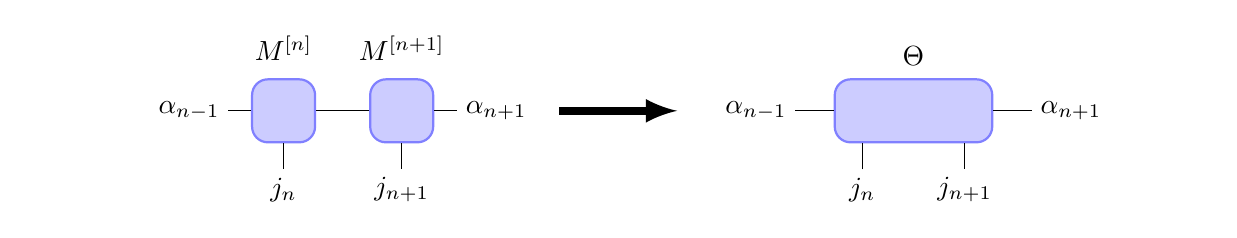
\begin{tikzpicture}[inner sep=1mm]
	\def \imgcenter {5.25};
	\def \imgwidth {15};
	\node[minimum width=\imgwidth cm] (fake) at (\imgcenter ,0) {};


    \node[tensor] (M1) at (1 , 0) {};
    \node[tensor] (M2) at (2.5 , 0) {};
	\node[tensor, minimum width=2cm] (sig) at (9, 0) {};
	
	\node (j1) at (1 ,-1) {$j_n$};
	\node (j2) at (2.5 ,-1) {$j_{n+1}$};
	\node (a1) at (-0.2 ,0) {$\alpha_{n-1}$};
	\node (a2) at (3.7 ,0) {$\alpha_{n+1}$};    
    
	\draw[-] (M1) -- (j1);
	\draw[-] (M1) -- (a1);
	\draw[-] (M1) -- (M2);
	\draw[-] (M2) -- (j2);
	\draw[-] (M2) -- (a2);
	
	
	\node (node1) at (8.35, -1) {$j_n$};
	\node (node2) at (9.65, -1) {$j_{n+1}$};
	\node (as1) at (7 ,0) {$\alpha_{n-1}$};
	\node (as2) at (11 ,0) {$\alpha_{n+1}$};
	
	\draw[-] (node1) -- (node1 |-  sig.south);
	\draw[-] (node2) -- (node2 |-  sig.south);
	\draw[-] (sig) -- (as1);
	\draw[-] (sig) -- (as2);		
	
	\draw[->, line width=1mm] (4.5,0) -- (6,0);
	
	\node (Mlab1) at (1,0.8) {$M^{[n]}$};
	\node (Mlab2) at (2.5,0.8) {$M^{[n+1]}$};
	\node (Siglab) at (9,0.7) {$\Theta$};
	
	
\end{tikzpicture}
	\end{subfigure}\\[.25cm]
	
	\begin{subfigure}{\textwidth}
		\centering
		\caption{\textbf{Solve eigenprobem:}}
		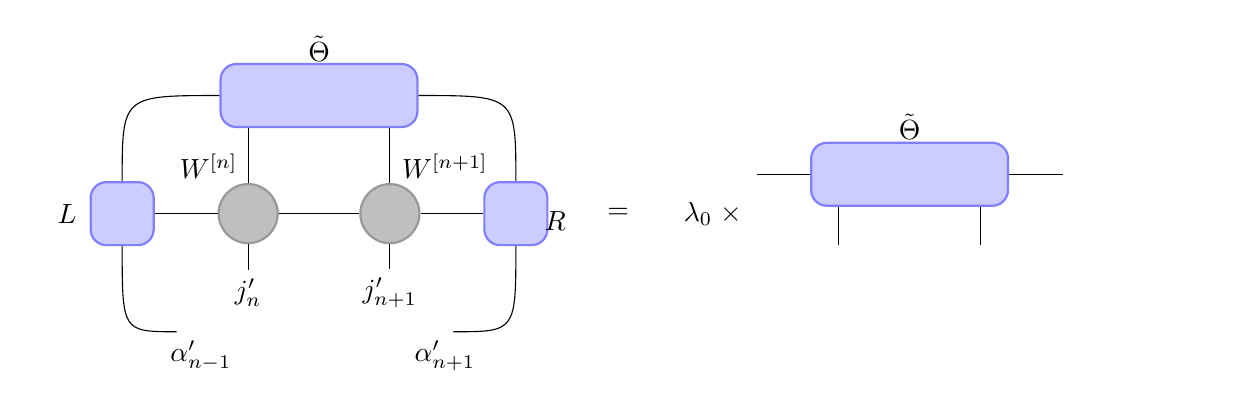
\begin{tikzpicture}[inner sep=1mm]
	\def \imgcenter {5.8};
	\def \imgwidth {15};
	\node[minimum width=\imgwidth cm] (fake) at (\imgcenter ,0) {};	
	
	
	\node[tensor, minimum width=2.5cm] (theta) at (2, 0) {};
	\node[operator] (W1) at (1.1,-1.5) {};
	\node[operator] (W2) at (2.9,-1.5) {};	
	
	\node (dummy1) at (0.3,-3) {};
 	\node (dummy2) at (3.6,-3) {};
	\node[tensor] (L) at (-0.5 , -1.5) {};
	\node[tensor] (R) at (4.5 , -1.5) {};    
    
    \draw[-] (dummy1.west) .. controls (-0.5, -3) .. (L.south);
    \draw[-] (dummy2.east) .. controls (4.5, -3) .. (R.south);
    \draw[-] (theta.west) .. controls (-0.5, 0) .. (L.north);
    \draw[-] (theta.east) .. controls (4.5, 0) .. (R.north);
	
	\draw[-] (L) -- (W1);
	\draw[-] (W1) -- (W2);
	\draw[-] (W2) -- (R);
	\draw[-] (W1) -- (W1 |-  theta.south);
	\draw[-] (W2) -- (W2 |-  theta.south);
	
	\node (j1) at (1.1 , -2.5) {$j_{n}'$};
	\node (j2) at (2.9 , -2.5) {$j_{n+1}'$};
	\draw[-] (W1) -- (j1);
	\draw[-] (W2) -- (j2);
	
	\node (a1) at (0.5 , -3.3) {$\alpha_{n-1}'$};
	\node (a2) at (3.6 , -3.3) {$\alpha_{n+1}'$};
	\node (Llab) at (-1.2 , -1.5) {$L$};
	\node (Rlab) at (5 , -1.6) {$R$};	
	\node (Thetalab) at (2 , 0.6) {$\tilde{\Theta}$};
	\node (W1lab) at (0.6 , -0.9) {$W^{[n]}$};
	\node (W2lab) at (3.6 , -0.9) {$W^{[n+1]}$};
	
	
	\def \offsetx {7.5};
	\def \offsety {-1};
	\node[tensor, minimum width=2.5cm] (theta2) at (2+\offsetx, \offsety) {};
	\node (d1) at (1.1 +\offsetx, -1+ \offsety) {};
	\node (d2) at (2.9 +\offsetx, -1 + \offsety) {};
	\node (d3) at (2+\offsetx - 1.25 - 0.8, 0+\offsety) {};
	\node (d4) at (2+\offsetx + 1.25 + 0.8, 0+\offsety) {};
	
	\draw[-] (d1) -- (d1 |-  theta2.south);
	\draw[-] (d2) -- (d2 |-  theta2.south);
	\draw[-] (d3) -- (theta2);
	\draw[-] (d4) -- (theta2);
	
	\node (Thetalab2) at (2 +\offsetx, 0.6 + \offsety) {$\tilde{\Theta}$};
	
	
	\node (eq) at (5.8 , -1.5) {$=$};
	\node (lambda) at (7 , -1.5) {$\lambda_0 \;  \times$};	
\end{tikzpicture}
	\end{subfigure}\\[.25cm]

	\begin{subfigure}{\textwidth}
		\centering
		\caption{\textbf{Unmerge:}}
		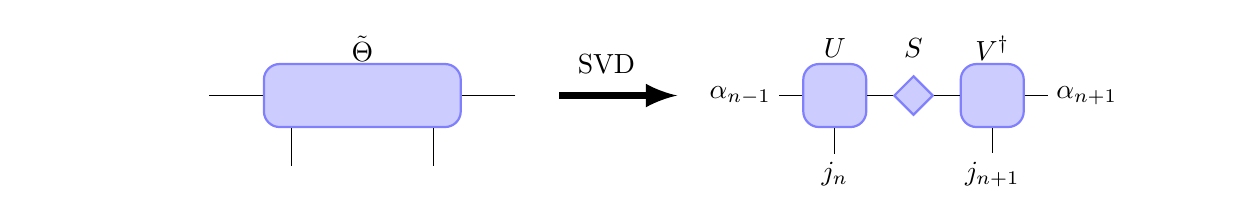
\begin{tikzpicture}[inner sep=1mm]	
	\def \center {2};
	\def \width {2.5};
	\def \offsetx {8};
	\def \xspace {1};
	\def \imgcenter {\offsetx -2.75};
	\def \imgwidth {15};
	\node[minimum width=\imgwidth cm] (fake) at (\imgcenter ,0) {};
	
	
	\node[tensor, minimum width=\width cm] (theta) at (\center, 0) {};
	
	\node (d1) at (\center - \width/2 + 0.35,-1) {};
	\node (d2) at (\center + \width/2 - 0.35,-1) {};
	\node (d3) at (\center - \width/2 - 0.8, 0) {};
	\node (d4) at (\center + \width/2 + 0.8, 0) {};
	
	\draw[-] (d1) -- (d1 |-  theta.south);
	\draw[-] (d2) -- (d2 |-  theta.south);
	\draw[-] (d3) -- (theta);
	\draw[-] (d4) -- (theta);	
	
	\node (thetalab) at (\center , 0 + 0.6) {$\tilde{\Theta}$};
	
	
	\node[tensor] (U) at (\offsetx , 0) {};
	\node[matrix] (S) at (\offsetx + \xspace, 0) {};
    \node[tensor] (V) at (\offsetx + 2*\xspace , 0) {};
	
	
	\node (j1) at (\offsetx ,-1) {$j_n$};
	\node (j2) at (\offsetx + 2*\xspace ,-1) {$j_{n+1}$};
	\node (a1) at (\offsetx -1.2 ,0) {$\alpha_{n-1}$};
	\node (a2) at (\offsetx + 2*\xspace +1.2 ,0) {$\alpha_{n+1}$};    
    
	\node (Ulab) at (\offsetx , 0.6) {$U$};
	\node (Slab) at (\offsetx + \xspace , 0.6) {$S$};
	\node (Vlab) at (\offsetx + 2*\xspace , 0.6) {$V^{\dag}$};    
    
	\draw[-] (U) -- (j1);
	\draw[-] (U) -- (a1);
	\draw[-] (U) -- (S);
	\draw[-] (V) -- (S);
	\draw[-] (V) -- (j2);
	\draw[-] (V) -- (a2);
	
	\draw[->, line width=1mm] (\offsetx-3.5 ,0) -- (\offsetx-2,0);
	\node (SVD) at (\offsetx-2.9 ,0.4) {SVD};
\end{tikzpicture}
	\end{subfigure}\\[.25cm]

	\begin{subfigure}{\textwidth}
		\centering
		\caption{\textbf{Update environments:}}
		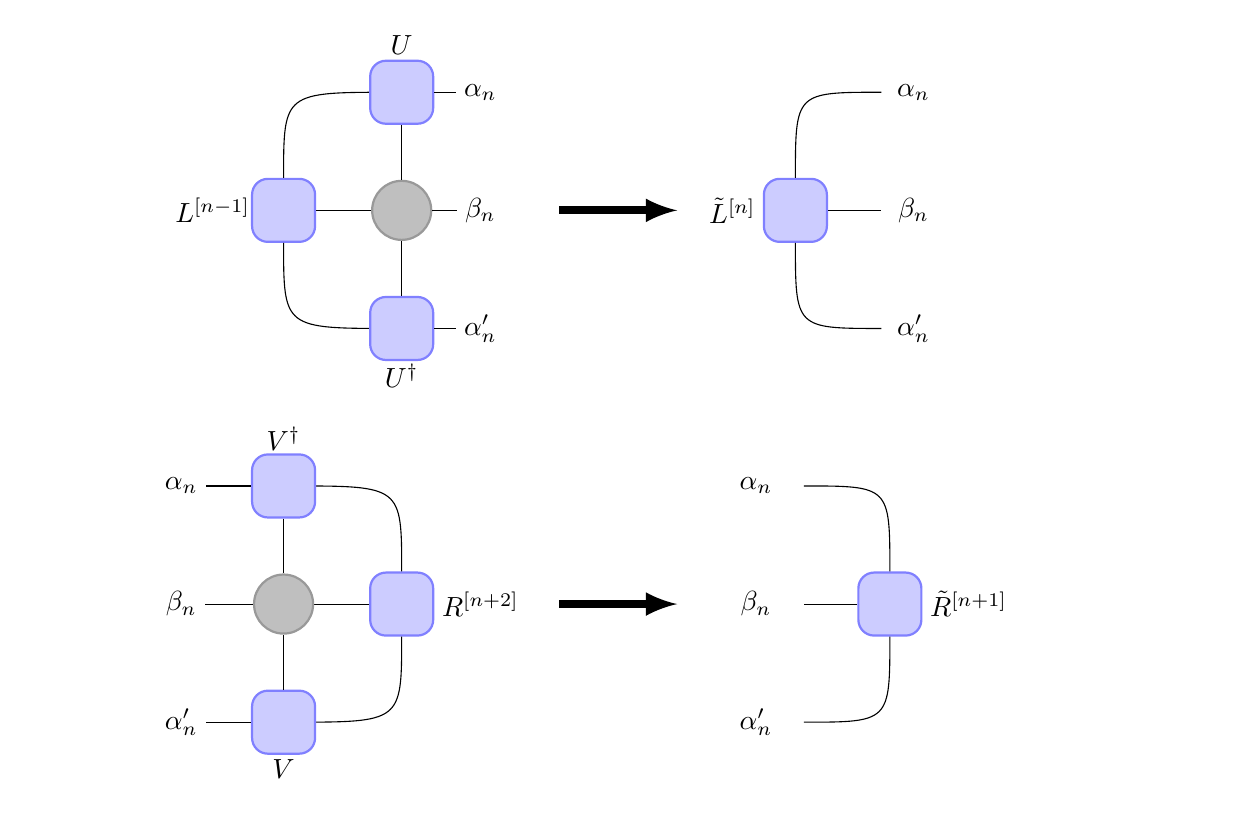
\begin{tikzpicture}[inner sep=1mm]
	\def \offsetx {6};
	\def \offsety {-5};
	\def \imgcenter {\offsetx -2.25};
	\def \imgwidth {15};
	\node[minimum width=\imgwidth cm] (fake) at (\imgcenter ,0) {};
	

	\Left{-0.5}{-1.5}{1.5};
	\node[tensor] (U1) at (1,0) {};	
	\node[tensor] (U2) at (1,-3) {};	
	\node[operator] (W) at (1,-1.5) {};

	\node (a1) at (2,0) {$\alpha_n$};
	\node (a2) at (2,-3) {$\alpha_n '$};
	\node (b) at (2,-1.5) {$\beta_n$};
	
	\draw[-] (U1) -- (W);
	\draw[-] (U2) -- (W);
	\draw[-] (U1) -- (a1);
	\draw[-] (U2) -- (a2);
	\draw[-] (W) -- (b);
	
	\node (L1) at (-1.4,-1.5) {$L^{[n-1]}$};
	\node (U1lab) at (1,0.6) {$U$};
	\node (U2lab) at (1,-3.6) {$U^{\dag}$};
	
	
	\draw[->, line width=1mm] (\offsetx-3 ,-1.5) -- (\offsetx-1.5,-1.5);
	
	
	\Left{\offsetx}{-1.5}{1.2};
	\node (L2) at (\offsetx -0.8,-1.5) {$\tilde{L}^{[n]}$};
	\node (a1) at (\offsetx+1.5,0) {$\alpha_n$};
	\node (a2) at (\offsetx+1.5,-3) {$\alpha_n '$};
	\node (b) at (\offsetx+1.5,-1.5) {$\beta_n$};
	
	%%----------------%%
	
	\Right{1}{-1.5 + \offsety}{1.5};
	\node[tensor] (U1) at (-0.5,0 + \offsety) {};	
	\node[tensor] (U2) at (-0.5,-3 + \offsety) {};	
	\node[operator] (W) at (-0.5,-1.5 + \offsety) {};

	\node (a1) at (-1.8,0 + \offsety) {$\alpha_{n}$};
	\node (a2) at (-1.8,-3 + \offsety) {$\alpha_{n} '$};
	\node (b) at (-1.8,-1.5 + \offsety) {$\beta_{n}$};
	
	\draw[-] (U1) -- (W);
	\draw[-] (U2) -- (W);
	\draw[-] (U1) -- (a1);
	\draw[-] (U2) -- (a2);
	\draw[-] (W) -- (b);
	
	\node (R1) at (2,-1.5 + \offsety) {$R^{[n+2]}$};
	\node (V1lab) at (-0.5,0.6 + \offsety) {$V^{\dag}$};
	\node (V2lab) at (-0.5,-3.6 + \offsety) {$V$};
	
	
	\draw[->, line width=1mm] (\offsetx-3 ,-1.5 + \offsety) -- (\offsetx-1.5,-1.5 + \offsety);
	
	
	\Right{\offsetx + 1.2}{-1.5 + \offsety}{1.2};
	\node (R2) at (\offsetx +2.2,-1.5 + \offsety) {$\tilde{R}^{[n+1]}$};
	\node (a1) at (\offsetx -0.5,0 + \offsety) {$\alpha_{n}$};
	\node (a2) at (\offsetx -0.5,-3 + \offsety) {$\alpha_{n} '$};
	\node (b) at (\offsetx -0.5,-1.5 + \offsety) {$\beta_{n}$};
\end{tikzpicture}
	\end{subfigure}
	
	
	\caption{\textit{Diagrammatic representation of the two-site update sequence for iterative ground state search. Step \textbf{(2)} optimizes with regard to two sites, but only a single site is updated to avoid getting stuck. In step \textbf{(4)}, when iterating left-to-right in the lattice, the left environment, $L^{[n]}$, is updated. The right environment, $R^{[n]}$, is updated when moving right-to-left.}}
	\label{fig:twoSiteUpdate}
\end{figure}

Some comments regarding the sequence are in order: The matrices of the eigenvalue problem have dimensions $( d^2 D^2 \times d^2 D^2)$, which is generally too much for exact diagonalization, however, since only the lowest eigenvalue is of interest, one can use an iterative eigensolver \cite{Lanczos}. Furthermore, if the MPS is not in the proper mixed-canonical form, the eigenvalue problem turns into a generalized eigenvalue problem, which can be numerically quite demanding. Thus, updating the left and right environments in step (4) is necessary, since it leads to great simplifications in step (2). Lastly, one could also consider just a single site when updating, however, this method is very prone to getting stuck \cite{White2005}. By updating two sites at once, one actually optimizes the bond between them. Hence, after updating the two sites, one must only iterate a single site. Optimization is done with regards to the current configuration, whereby it depends on previous updates. To compensate for this, one must sweep through the entire system multiple times, which leads to the following algorithm for iterative ground state search, which follows the structure of the DMRG algorithm:

\begin{algorithm}
\begin{algorithmic}
\caption{Iterative ground state search (DMRG)}
\State Choose $\ket{\psi}$ right-normalized.
\State Calculate tensor $R^{[i]}$ iteratively for $i = L \ldots 1$.
\While{Stopping criteria not met} 
	\For{$n = 1 \ldots L-1$} \Comment{Left sweep}
		\State Perform two-site update on $M^{[n]}$ and $M^{[n+1]}$.
		\State Update $L^{[n]}$ according to eq. \eqref{eq:updateLeft}
	\EndFor
	\For{$n = L-1 \ldots 1$} \Comment{Right sweep}
		\State Perform two-site update on $M^{[n]}$ and $M^{[n+1]}$.
		\State Update $R^{[n]}$ according to eq. \eqref{eq:updateRight}
	\EndFor
\EndWhile
\end{algorithmic}
\end{algorithm}


\subsection{Applications of DMRG Algorithm on Bose-Hubbard Systems} \label{chap:CondFrac}
The DMRG algorithm has proven itself to be one of the most powerful methods for describing ground states in one-dimensional systems. This will be illustrated here by characterizing equilibrium properties of the Bose-Hubbard phases. First, the DMRG algorithm is compared to exact diagonalization methods applied on small systems, where the eigenstates of the Hamiltonian are extracted directly by diagonalizing the Hamilton matrix. However, exact diagonalization is only applicable on small systems, due to the exponential scaling of the Hilbert space \cite{Vidal2003}. Referring back to eq. \eqref{eq:HilberSpaceScaling}, a Bose-Hubbard system with 10 sites and unit occupation has a Hilbert space dimension around $D_{\mathcal{H}}^{(L = 10)} = 9.2 \cdot 10^{4}$. The corresponding Hamiltonian matrix has a size of $D_{\mathcal{H}} \times D_{\mathcal{H}}$, although it is quite sparse, which enables sparse eigensolvers to find the ground state through exact diagonalization.
However, a 20-site Bose-Hubbard system will have a Hilbert space dimension of $D_{\mathcal{H}}^{(L = 20)} = 6.9 \cdot 10^{10}$, which is far outside the reach of exact diagonalization. Meanwhile, the DMGR algorithm can comfortably find very accurate ground states in such large Hilbert spaces. In fact, for the analysis presented here, systems up to 50 lattice sites are examined. Such systems have Hilbert spaces of astronomical dimensions $D_{\mathcal{H}}^{(L = 50)} = 5.0 \cdot 10^{28}$, however, as long as the ground state obeys an area law, the DMRG algorithm can easily find it in only a few sweeps through the lattice.


\subsubsection{Approximating critical point through condensate fraction}

According to the Penrose-Onsager criterion, a system is in the superfluid phase if and only if the largest eigenvalue, $\lambda_1$, of the single-particle density matrix, $\rho^{(1)}$, is macroscopic
\begin{equation}
	f_c = \frac{\lambda_1}{N_p} > 0 \; ,
	\label{eq:condensateFraction}
\end{equation} 
where $f_c$ is the condensate fraction \cite{PenroseOnsager}. The entries of the density matrix are given by the single-particle correlations
\begin{equation}
	\rho_{i,j}^{(1)} = \bra{\psi} \hat{a}_{i}^{\dag} \hat{a}_{j} \ket{\psi} \; ,
	\label{eq:DensityMatrixEntry}
\end{equation}
where $\ket{\psi}$ is the ground state of the system. The ground state of the system was found using both a version of the DMRG algorithm implemented in the ITensor library \cite{ITensor} and an exact diagonalization script also used in \cite{MajaJulie}. If the state is parameterized through a tensor network, the correlations can be efficiently evaluated using the procedures detailed in Section \ref{sec:correlationFunctions}.

The condensate fraction can be used to determine which phase dominates the system, as
\begin{align}
	\lim_{N_p \to \infty} f_{c}^{\mathrm{SF}} &\to 1 \label{eq:SF_lim} \\
	\lim_{N_p \to \infty} f_{c}^{\mathrm{MI}} &\to 0 \; , \label{eq:MI_lim}
\end{align}
when the filling-fraction, $n = N_p/L$, is held constant. Thus, one should be able to recognize the phase of a Bose-Hubbard system at a given point $U/J$ from the corresponding condensate fraction.
Therefore, the condensate fraction was calculated using ground state at various fractions $U/J$ for a series of system sizes. The results of this calculation are shown in figure \ref{fig:CondensateFraction}.
\begin{figure}[h!]
    \centering
    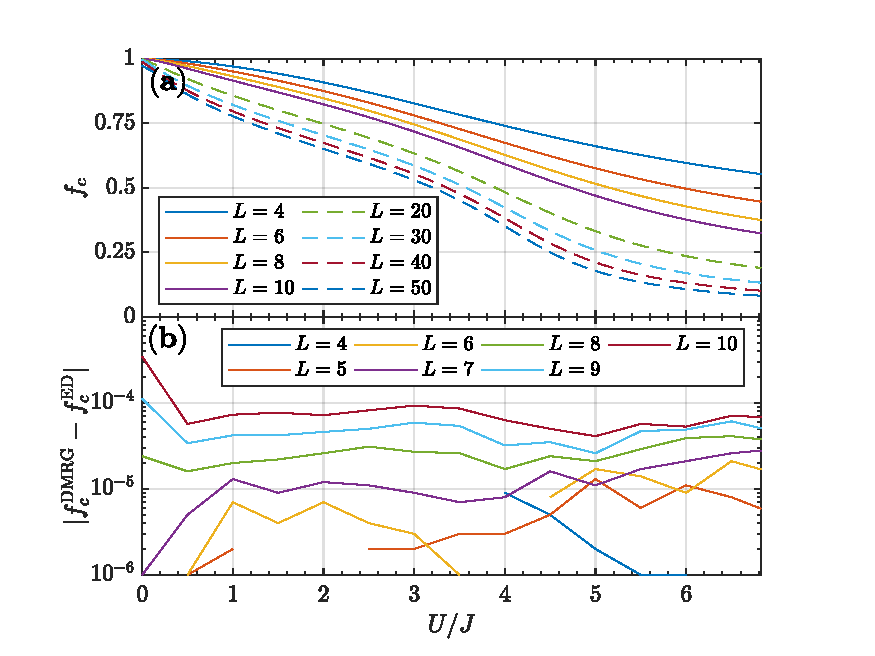
\includegraphics[width=0.9\textwidth]{Figures/CondensateFractionCompare.pdf}
 \caption{Condensate fraction of Bose-Hubbard system as function of $U/J$ for various system sizes. \textbf{(a)} Condensate fraction calculated using DMRG algorithm with a maximum bond dimension $D = 200$. The results were achieved through 5 DMRG sweeps, with exception of the $U/J \sim 0$ limit, where 20 sweeps were used. The dashed lines mark system sizes outside the scope of exact diagonalization. \textbf{(b)} Absolute difference between condensate fractions obtained through DMRG and exact diagonalization.}
 \label{fig:CondensateFraction}
\end{figure}

In order to confirm the accuracy of the DMRG algorithm, the condensate fraction calculated for system sizes $L =  4 , \ldots , 10 $ were compared to results obtained through exact diagonalization, which can be seen in figure \ref{fig:CondensateFraction}(b). Clearly, the two methods produce very similar results when applied to small systems.

Meanwhile, figure \ref{fig:CondensateFraction}(a) displays the condensate fraction for various $U/J$ calculated using the DMRG algorithm. In the limit $U/J = 0$, the condensate fraction is unit for the smaller systems, confirming the system is indeed in the superfluid phase. The condensate fraction never reaches zero as $U/J$ increases, since this is only achieved in the thermodynamic limit. However, the condensate fraction does decrease as the particle number increases, which is the behavior expected from eq. \eqref{eq:MI_lim}.
Note, in the superfluid limit the condensate fraction does not quite reach unit for the largest, $L = 50$, system. For large systems the superfluid phase is gapless, whereby the ground state no longer follows an area law. A small interaction will cause the spectrum of the superfluid to become gapped for small system, as the otherwise gapless spectrum is a consequence of particles delocalizing over \textit{many} sites. However, in the $U/J = 0$ limit for large systems, the spectrum will have exponentially small gaps, whereby the area laws will break down. Hence, the DMRG algorithm has to search a much larger part of the Hilbert space for the ground state, which greatly reduces its efficiency. A possible solution to this issue is using more sweeps in the ground state search. Figure \ref{fig:sweepdependence} displays the condensate fraction in the superfluid limit as a function of number of sweeps. Allowing the DMRG algorithm to perform additional search-sweeps clearly causes an improvement in the ground state description.\\ 
\begin{figure}[h!]
    \centering
    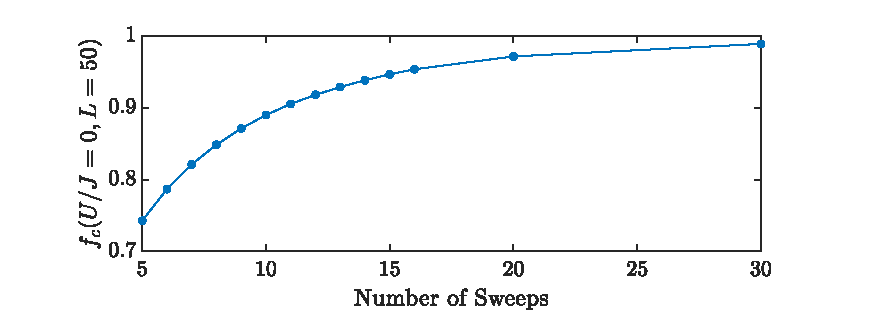
\includegraphics[width=0.9\textwidth]{Figures/CFsweeps.pdf}
    \caption{Condensate fraction as a function of number of sweeps of the DMRG algorithm in the superfluid limit. A max bond dimension of $D = 250$ was used.}
    \label{fig:sweepdependence}
\end{figure}

In \cite{Kuhner2000} the critical point of the phase transition between the superfluid and Mott-insulator was determined as $\left( {U}/{J} \right)_{crit} = 3.37$ by examining the correlations of the systems. Alternatively, one could determine the critical point through the condensate fraction. In the thermodynamic limit one would expect the condensate fraction to drop to zero, as the critical point is reached (as observed in 2D by \cite{Spielman2008}).
Due to the finite system-sizes examined here, no such sharp indication of a phase transition is present in figure \ref{fig:CondensateFraction}(a). Nevertheless, the condensate fraction does appear to decrease faster around $U/J \approx 4$. As this decrease becomes more pronounced for larger systems, it is reasonable to conclude from figure \ref{fig:CondensateFraction}(a) that $\left( {U}/{J} \right)_{crit} \in [ 2.5 , 5 ]$. While this is not an exact position of the critical point, it is already a much better approximation than the mean-field result of $\left( U/J \right)_{crit}^{MF} = 11.66$ derived in Section \ref{sec:MeanFieldDiagram}.


\subsubsection{Single-particle correlations of superfluid and Mott-insulator}

\begin{figure}[h!]
    \centering
    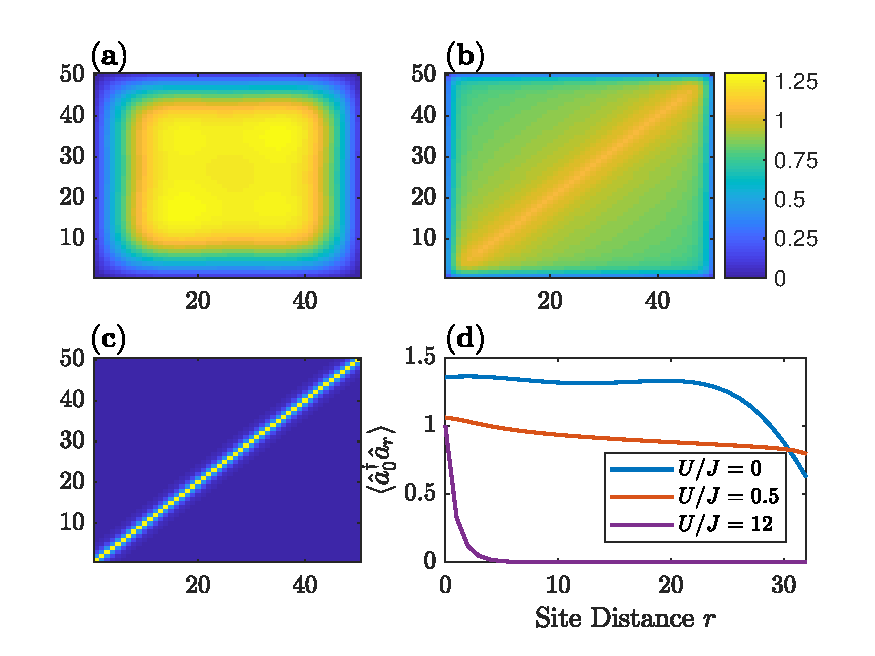
\includegraphics[width=0.9\textwidth]{Figures/DensityMatrices.pdf}
    \caption{Density matrices \eqref{eq:DensityMatrixEntry} of a 50 site system for \textbf{(a)} $U/J = 0$, \textbf{(b)} $U/J = 0.5$, and \textbf{(c)} $U/J = 12$. \textbf{(d)} Single-particle correlation function extracted from the entries of the 15th row of the density matrices. The correlations are plotted as a function of distance from the diagonal, $r$. }
    \label{fig:DensityMatrices}
\end{figure}

Correlation functions can be used to characterize quantum systems. Single-particle correlations decay exponentially in a Mott-insulator, while they for superfluids decay following a power-law 
\begin{equation}
	\braket{\hat{a}_{i}^{\dag} \hat{a}_{j}} \sim |i - j|^{-K_b /2} \; ,
	\label{eq:superfluidCorrelation}
\end{equation}
where $K_b$ is the Tomonaga-Luttinger parameter \cite{characPhases}. To illustrate the very different properties of the two Bose-Hubbard phases, the density matrices \eqref{eq:DensityMatrixEntry} for $U/J = 0, \; 0.5, \; 12$ and $L = 50$ were calculated using ground states obtained through the DMRG algorithm. 

Figure \ref{fig:DensityMatrices}(a) shows the density matrix in the superfluid limit $U/J = 0$. In the superfluid phase the energy of the system is minimized by de-localizing the particles across the entire lattice, whereby the atoms are essentially described by Bloch waves. Therefore, the single-particle correlations, $\bra{\psi} \hat{a}_{i}^{\dag} \hat{a}_{j} \ket{\psi}$, are very long-ranged. However, due to the open boundary conditions, particles can only tunnel in one direction at the outer sites, which effectively causes a depletion of their population. This can be seen from the diagonal of the density matrix, which describes the population at each site
\begin{equation}
	\bra{\psi} \hat{a}_{i}^{\dag} \hat{a}_{i} \ket{\psi} = \braket{\psi | \hat{n}_i | psi} \; .
\end{equation}
The depletion of population at the outer sites causes the single-particle correlations to exhibit a sharp decrease near the edges of the system.

Meanwhile, figure \ref{fig:DensityMatrices}(b) illustrates the density matrix for $U/J = 0.5$. The ground state is still in the superfluid phase, but the system now has finite interactions. The finite interactions causes the atoms to no longer condense into a single momentum state. This spread in momentum-space results in the atoms no longer being completely de-localized in real-space, which is noticeable from the visible diagonal of the density matrix. The stronger localization due to interactions results in a much smaller effect of boundary conditions compared to the non-interacting case. 

Finally, the density matrix plotted in figure \ref{fig:DensityMatrices}(c) belongs to a system in the Mott-insulating regime. Here, the particles are highly localized, which is apparent from the dominating diagonal elements. Furthermore, in the Mott-insulator limit, interactions between sites are highly suppressed, whereby the single-particle correlations decay exponentially. For ground states even deeper in the Mott regime, the correlations would be even further suppressed, whereby the correlation length would decrease to even fewer sites. 

To quantitatively compare the correlations of the different states, the single-particle correlation function were extracted from the density matrices. Figure \ref{fig:DensityMatrices}(d) displays the correlations as function of distance from a reference site in the lattice.
Starting with the $U/J = 0.5$ system, the ground state is clearly in the superfluid phase, as the correlations are very long-ranged and decay following a power law \eqref{eq:superfluidCorrelation}. This should also be the case in the $U/J = 0$ limit, however, the correlation function clearly does not exhibit a power-law behavior. The reason for this is two-fold: First, correlation functions are given by an exponential series in the MPS representation, which causes a poor description of very long-ranged correlation. This is further elaborated in Appendix \ref{sec:CorrelationLength}. Secondly, in the limit of large systems and negligible interactions the superfluid spectrum becomes gapless, whereby the DMRG algorithm fails to find the exact ground state. Finally, the correlation function for the $U/J = 12$ state is clearly exponential, therefore confirming that the state is in the Mott-insulator phase.



\section{Time Evolution of Matrix Product States}
Several algorithms for time evolving matrix product states exist, however, they all origin from the same ideas proposed in \cite{Vidal2003,Vidal2004}. The most widely used of these algorithms is the tDMRG algorithm \cite{Daley2004}, which gets its name from its similarity with the ground state search algorithm described in section \ref{sec:DMRG}. The tDMRG algorithm has been utilized in several instances to simulate the dynamics of one-dimensional systems \cite{Verstraete2004,Vznidarivc2008,Cazalilla2002}, and it has even been previously used in conjunction with the CRAB algorithm to perform optimal control of the superfluid to Mott-insulator phase transition \cite{FrankBloch,Doria2011}.

Although the standard algorithms for time evolution are quite efficient, further improvements can be made to the algorithms by tailoring them to the problem at hand. Therefore, a modified version of the tDMRG algorithm is proposed in Section \ref{sec:modTMDRG}, which directly utilizes the properties of the Bose-Hubbard Hamiltonian.


\subsection{The tDMRG Algorithm}
Consider the time evolution of a quantum state
\begin{equation}
	\ket{\psi (t)} = \hat{\mathcal{U}}(t) \ket{\psi (0)} \; ,
\end{equation}
where $\hat{\mathcal{U}}(t) = \e^{ - \im \hat{H} t }$ is the time evolution operator. 
Time evolution of matrix product states is similarly to the ground state search, as the bonds between the tensors are evolved rather than the tensors themselves \cite{Vidal2003,Vidal2004}. Thus, the time evolution operator must be decomposed into two-site tensors. The simplest realization of this is achieved by considering a Hamiltonian containing only nearest-neighbour interactions.
Assume the Hamiltonian is a sum of two-site operators of the form $\hat{H} = \sum_{n} \hat{h}^{[n , n+1]}$. One can decompose this into a sum over even and odd bonds \cite{Vidal2004}
\begin{equation}
	\hat{H} = \hat{H}_{\mathrm{odd}} \; + \; \hat{H}_{\mathrm{even}} = \sum_{n \; \mathrm{odd}} \hat{h}^{[n , n+1]} \; + \; \sum_{n \; \mathrm{even}} \hat{h}^{[n , n+1]} \; .
\end{equation}  
Exponentiating the Hamiltonian is non-trivial due to the non-commutativity of the operators
\begin{equation}
	[ \hat{h}_{\mathrm{odd}}^{[n , n+1]} \; , \; \hat{h}_{\mathrm{even}}^{[n , n+1]} ] \neq 0 \; .
\end{equation}
Considering a small time slice, $\Delta t$, the exponentiation can be achieved through the Trotter-Suzuki expansion \cite{Suzuki1991}. To first order this reads
\begin{equation}
	\e^{- \im \hat{H} \; \Delta t} = \e^{- \im \hat{H}_{\mathrm{odd}} \; \Delta t } \e^{- \im \hat{H}_{\mathrm{even}} \; \Delta t} \; + \; \;  \mathrm{O}(\Delta t^2) \; ,
\end{equation}
where the error is due to the non-commutativity of the bond Hamiltonians. Thus, the time evolution operator can be expressed as the product
\begin{equation}
	\hat{\mathcal{U}}(\Delta t) \approx \left( \prod_{n \; \mathrm{odd}} \hat{\mathcal{U}}^{[n,n+1]} (\Delta t) \right) \left( \prod_{n \; \mathrm{even}} \hat{\mathcal{U}}^{[n,n+1]} (\Delta t) \right) \; , \label{eq:SuzukiTrotter1stOrder}
\end{equation}
where
\begin{equation}
	\hat{\mathcal{U}}^{[n,n+1]} (\Delta t) = \e^{- \im \hat{h}^{[n , n+1]} \; \Delta t } \; .
\end{equation}
The result is an MPO performing an infinitesimal time step on the odd bonds, and another MPO evolving the even bonds. An illustration of eq. \eqref{eq:SuzukiTrotter1stOrder} is shown in Figure \ref{fig:oddevenops}.
\begin{figure}[h!]
	\centering
	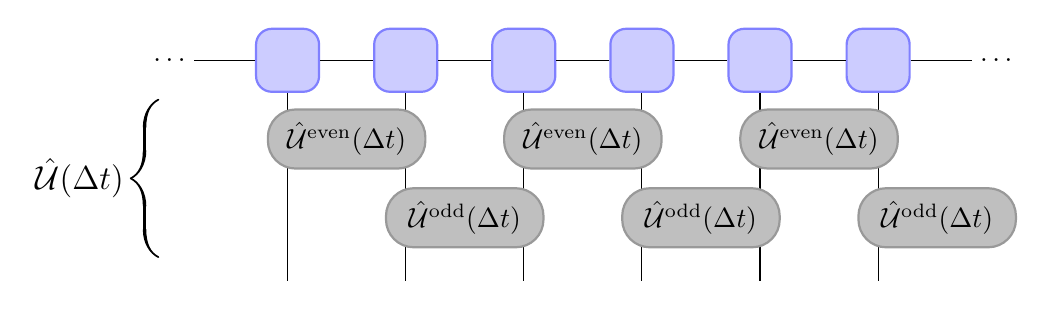
\begin{tikzpicture}[inner sep=1mm]
	\def \reldist {1.5};
	\def \numb {6};
	\def \wid {2}

	\foreach \i in  {1,...,\numb} {
		\node[tensor] (t\i) at (\i * \reldist, 0) {};
		\draw[-] (t\i) -- (\i * \reldist , -2.8);	
	};
	
	\foreach \i in {1,...,5} {
        \pgfmathtruncatemacro{\iplusone}{\i + 1};
        \draw[-] (t\i) -- (t\iplusone);
	};
	
	\foreach \i in {1,3,5} {
        \node[twositeop, minimum width= \wid cm] (op\i) at (\reldist*\i + \wid/2 -0.25,-1) {$\hat{\mathcal{U}}^{\mathrm{even}} (\Delta t)$};
	};
	
	\foreach \i in {2,4,6} {
        \node[twositeop, minimum width= \wid cm] (op\i) at (\reldist*\i + \wid/2 -0.25,-2) {$\hat{\mathcal{U}}^{\mathrm{odd}} (\Delta t)$};
	};	
	
	\node (dot1) at (0,0) {$\dots$};
	\node (dot2) at (\numb * \reldist + \reldist,0) {$\dots$};
	\draw[-] (t1) -- (dot1);
	\draw[-] (t\numb) -- (dot2);
	
	\draw[decoration={calligraphic brace,amplitude=10pt}, decorate, line width=1.25pt, xshift=-4pt, yshift=0pt]
(0, -2.5) -- (0,-0.5) node [black,midway,xshift=-1.0cm] 
{\large $\hat{\mathcal{U}} ( \Delta t)$};
	
\end{tikzpicture}
	\caption{Approximation of each time step $\Delta t$ using a Trotter-Suzuki expansion, such that the time evolution operator is expressed as a product of unitary two-site operators.}
	\label{fig:oddevenops}
\end{figure}
The tDMRG algorithm describes the most efficient and accurate way of contracting the tensor network detailed in figure \ref{fig:oddevenops}. The algorithm gets its name from its similarity with the DMRG algorithm detailed in section \ref{sec:DMRG}. In fact, the merge and unmerge procedure of the two algorithms are completely identical, whereby they only differ in the steps of applying the operator and proceeding to the next site. The following procedure details a time evolution step of the $n$'th bond \cite{schollwock}.

\subsubsection{Infinitesimal time-step update for tDMRG}
\begin{enumerate}
\item
\textbf{Merge:} Contract tensors $M^{[n]}$ and $M^{[n+1]}$ over the bond $\alpha_{n}$ creating a two-site tensor $\Theta^{j_n , j_{n+1}}$.

\item
\textbf{Apply unitary:} The two-site time evolution operator, $\hat{\mathcal{U}}^{[n, n+1]}$, is applied to $\Theta^{j_n , j_{n+1}}$
\begin{equation}
	\tilde{\Theta}_{\alpha_{n-1} , \alpha_{n+1}}^{j_n , j_{n+1} } = \sum_{j_n ', j_{n+1}'} \mathcal{U}^{j_n  j_{n+1} , j_n '  j_{n+1}'} \; \Theta_{\alpha_{n-1} , \alpha_{n+1}}^{j_n ', j_{n+1} ' } \; .
\end{equation}

\item
\textbf{Unmerge:} Reshape $\tilde{\Theta}_{\alpha_{n-1} , \alpha_{n+1}}^{j_n ', j_{n+1} '}$ to a matrix and decompose it through an SVD. Applying $\hat{\mathcal{U}}^{[n, n+1]}$ causes an increase in bond dimension, $D \rightarrow d^2 D$, which must be truncated by keeping only the $D$ largest singular values from the SVD. 

\item
\textbf{Progress:}  Next, the center cite of the MPS must be shifted by two, in order to update the next even (odd) bond. This is achieved by merging tensors $M^{[n+1]}$ and $M^{[n+2]}$ and performing a second SVD, while reshaping the resulting $U$-matrices to left-normalised tensors to retain the canonical form. The product of the second SVD must be truncated as well, however, no loss of information will occur, as the Schmidt rank of the matrix $S$ will be at most $D$ following the first SVD. 
\end{enumerate}
Following the procedure above will leave the MPS in position for application of the unitary $\hat{\mathcal{U}}^{[n+2 , n+3]}$. The efficiency of the tDMRG algorithm depends on the sequence in which bonds are evolved. A simple, yet effective way is iterating from left to right when evolving even bonds, while iterating right to left when evolving odd bonds. Thereby, the centered cite of the mixed-canonical form is moved continuously through the MPS, rather than having to be reset when reaching the end of the system.

It has been shown that the area law scaling of entanglement of an initial state will remain true even for longer times \cite{Bravyi2006,Eisert2006}. Simultaneously, the pre-factor of the area-law is expected to grow exponentially \cite{Schuch2008}. Therefore, the maximum bond dimension, $D$, kept in each iteration of the tDMRG algorithm must be chosen sufficiently high in order to properly capture the relevant dynamics of the system. Alternatively, one can truncate the bond dimensions of the tensors according to some eigenstate-contribution threshold, $\epsilon_t$. While this will ensure a consistent description of the state throughout the simulation, the bond dimension may grow very large thereby causing a significant decrease in the efficiency of the algorithm. Thus, analyzing the evolution of the bond dimension is imperative for the success of the simulation when examining phenomena of high entanglement such as phase transitions.

Although the tDMRG algorithm is a very powerful algorithm, an even higher efficiency can be achieved when tailoring the algorithm to the system - in this case the Bose-Hubbard model. Thus, the Hamiltonian contains both nearest-neighbour and on-site terms. Furthermore, the Hamiltonian is time dependent, since the lattice depth is varied when driving a phase transition, whereby the propagator at each time step is different. The following algorithm is a modification of the tDMRG algorithm, which is tailored for conducting optimal control using the Bose-Hubbard Hamiltonian.


\subsection{Modified Time Evolution Algorithm for Bose-Hubbard Model}
\label{sec:modTMDRG}
The control problem solved in this thesis consist of dynamically transferring a superfluid ground state to a Mott-insulating ground state. Thus, the Hamiltonian is time-dependent, whereby it must be exponentiated for every time-step to create the propagators required for the time-evolution. Furthermore, any optimization of the control sequence will require the corresponding propagators to be re-calculated. Thus, the computational time of the propagators must be taken into account. Typically, operators are exponentiated through series expansions, however, this is in general a rather expensive operation. Therefore, choosing control-Hamiltonians which are easy to exponentiate is often an advantage.

The phase of the Bose-Hubbard model depends on the ratio $U/J$, where $U$ is the interaction matrix element \eqref{eq:BHparamU}, and $J$ is the tunneling matrix element \eqref{eq:BHparamJ}. Both parameters are dependent of the lattice depth, which therefore has been used as control function in previous studies \cite{FrankBloch,Doria2011}. Exponentiating the tunneling Hamiltonian is non-trivial, however, the interaction Hamiltonian is diagonal, whereby the propagator can be computed by simply exponentiating the elements of the matrix. Thus, choosing the ratio $U/J$ as the control function and working in units of $J$ significantly simplifies the calculation of propagators, as the tunneling propagator remains constant. Employing a second-order Suzuki-Trotter expansion
\begin{equation}
	\exp\left( \text{-}i ( \hat{H}_J + \hat{H}_U  ) \Delta t \right) = \exp\left( \text{-} i \hat{H}_U \Delta t /2  \right) \exp\left( \text{-} i \hat{H}_J \Delta  t \right) \exp\left( \text{-} i \hat{H}_U \Delta t /2  \right) + O(\Delta t^3) \; ,
	\label{eq:SuzukiTrotter}
\end{equation}
allows separate exponentiation of the two parts of the Bose-Hubbard Hamiltonian, whereby only the interaction needs to be updated. Again, the error is due to the non-commutativity of operators. Thereby, the expanded propagator reads
\begin{equation}
	\hat{\mathcal{U}} (\Delta t) = \left( \prod_{i = 1}^{L} \hat{\mathcal{U}}_{U}^{[i]} \right) \left( \prod_{i \; \mathrm{odd}}^{L} \hat{\mathcal{U}}_{J}^{[i,i+1]}  \right) \left( \prod_{i \; \mathrm{even}}^{L} \hat{\mathcal{U}}_{J}^{[i,i+1]}  \right) \left( \prod_{i = 1}^{L} \hat{\mathcal{U}}_{U}^{[i]} \right) \; ,
\end{equation}
where the site-specific propagators, or gates, are given by
\begin{align}
	\hat{\mathcal{U}}_{J}^{[i,i+1]} &= \exp \left( \text{-} i J ( \hat{a}_{i}^{\dag} \hat{a}_{i+1} + \hat{a}_{i+1}^{\dag} \hat{a}_{i} ) \Delta t \right) \\
	\hat{\mathcal{U}}_{U}^{[i]} &= \exp \left( \text{-} i \frac{U}{2} \hat{n}_i (\hat{n}_i -1) \Delta t /2 \right) \; .
\end{align}
\begin{figure}[h!]
	\centering
	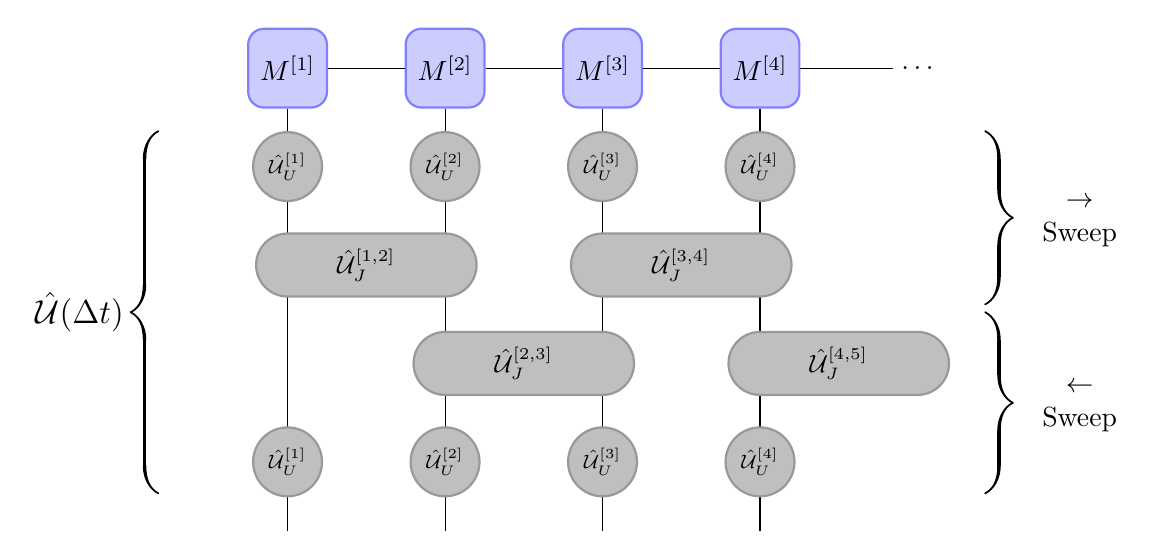
\begin{tikzpicture}[inner sep=1mm]
\def \reldist {2};
\def \numb {4};
\def \wid {2.8};
\def \size {1.0};
\def \hi {0.8};
\def \vert {1.25};
\def \rad {0.4};

	
\foreach \i in  {1,...,\numb} {
	\node[tensor,minimum width= \size cm,minimum height= \size cm, rounded corners = 0.2cm] (A\i)
	at (\i * \reldist, 0) {$M^{[ \i ]}$};
	\draw[-] (A\i) -- (\i * \reldist , -4.7*\vert);	
};

\foreach \i in {1,...,3} {
    \pgfmathtruncatemacro{\iplusone}{\i + 1};
    \draw[-] (A\i) -- (A\iplusone);
};


\foreach \i in  {1,...,\numb} {
	\node[operator,minimum width= \hi cm,minimum height= \hi cm] (op\i)
	at (\i * \reldist, -\vert )
	{\scriptsize $\hat{\mathcal{U}}_{U}^{[ \i ]}$};	
};

\foreach \i in {1,...,\numb} {
	\pgfmathtruncatemacro{\j}{\i + 1};
    \node[twositeop, minimum width= \wid cm,minimum height= \hi cm,rounded corners = \rad cm] (eop\i)
    at (\reldist*\i + \reldist/2, {-2*\vert - Mod(\j,2) *\vert })
    {\small $\hat{\mathcal{U}}_{J}^{[ \i , \j ]} $};
};

\foreach \i in  {1,...,\numb} {
	\node[operator,minimum width= \hi cm,minimum height= \hi cm] (op\i)
	at (\i * \reldist, -4*\vert )
	{\scriptsize $\hat{\mathcal{U}}_{U}^{[ \i ]}$};	
};




\draw[decoration={calligraphic brace,amplitude=10pt}, decorate, line width=1.25pt, xshift=-4pt, yshift=0pt]
(0.5, -4*\vert -0.4) -- (0.5,-0.8) node [black,midway,xshift=-1.0cm] 
{\large $\hat{\mathcal{U}} ( \Delta t)$};


\draw[decoration={calligraphic brace,amplitude=10pt,mirror}, decorate, line width=1.25pt, xshift=-4pt, yshift=0pt]
(\numb * \reldist + 3, -2*\vert -0.5) -- (\numb * \reldist + 3,-0.8) node [black,midway,xshift=1.2cm] 
{\normalsize \begin{tabular}{c}
				$\rightarrow$ \\
				Sweep \\
			  \end{tabular} };


\draw[decoration={calligraphic brace,amplitude=10pt,mirror}, decorate, line width=1.25pt, xshift=-4pt, yshift=0pt]
(\numb * \reldist + 3, -4*\vert -0.4) -- (\numb * \reldist + 3,-2*\vert -0.6) node [black,midway,xshift=1.2cm] 
{\normalsize \begin{tabular}{c}
				$\leftarrow$ \\
				Sweep \\
			  \end{tabular} };


\node (dot2) at (\numb * \reldist + 2,0) {$\dots$};
\draw[-] (A\numb) -- (dot2);
	
	
\end{tikzpicture}
	\caption{Tensor diagram depicting a single time step of the modified tDMRG algorithm. The tensors of the upper part of the network are contracted with the MPS while sweeping from left to right, whereas the lower part is applied with a right-to-left sweep.}
	\label{fig:ModifiedTEBD}
\end{figure}
A single time step, $\Delta t$, using the expanded operator is represented diagrammatically in figure \ref{fig:ModifiedTEBD}. At first glance, the tensor network resulting from the Suzuki-Trotter expansion may seem rather extensive, however, it can be contracted in a very efficient manner. The upper part of the network is contracted in a left-to-right sweeping manner, where the position of the center cite, and thereby the normalization of the MPS, is pushed to the right following each step. Likewise, the lower part of the network is contracted though a right-to-left sweep such that the MPS returns to its original form centered on the first site after applying the final operator. Thereby, the MPS is immediately ready for the subsequent time-propagation.\\
\begin{figure}[h!]
\centering % <-- add this
\begin{subfigure}[b]{0.4\textwidth}
	\caption{}  
  	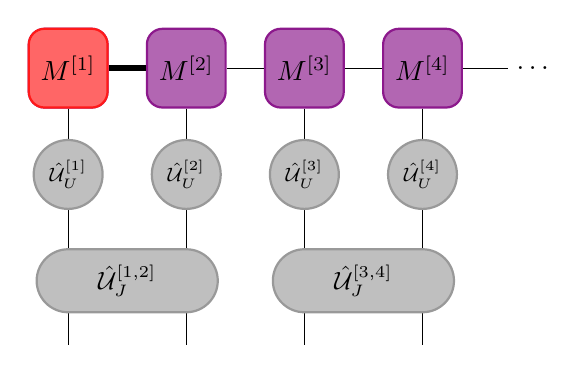
\begin{tikzpicture}[inner sep=1mm]
\def \reldist {1.5};
\def \numb {4};
\def \wid {2.3};
\def \size {1.0};
\def \hi {0.8};
\def \rad {0.4};
\def \vert {1.35};


\foreach \i in  {1,...,\numb} {
	\node[tensorr,minimum width= \size cm,minimum height= \size cm, rounded corners = 0.2cm] (A\i)
	at (\i * \reldist, 0) {$M^{[ \i ]}$};
	\draw[-] (A\i) -- (\i * \reldist , -2.5*\vert);	
};

\foreach \i in {1,...,3} {
    \pgfmathtruncatemacro{\iplusone}{\i + 1};
    \draw[-] (A\i) -- (A\iplusone);
};

\node[tensorc,minimum width= \size cm,minimum height= \size cm, rounded corners = 0.2cm] (C) at (1 * \reldist, 0) {$M^{[1]}$};


\foreach \i in  {1,...,\numb} {
	\draw[-] (A\i) -- (\i * \reldist , -2.6 *\vert);	
};

\draw[-,line width=0.8mm] (A1) -- (A2);

\foreach \i in  {1,...,\numb} {
	\node[operator,minimum width= \hi cm,minimum height= \hi cm] (op\i)
	at (\i * \reldist, -\vert)
	{\scriptsize $\hat{\mathcal{U}}_{U}^{[ \i ]}$};	
};

\foreach \i in {1,3} {
	\pgfmathtruncatemacro{\j}{\i + 1};
    \node[twositeop, minimum width= \wid cm,minimum height= \hi cm,rounded corners = \rad cm] (top\i)
    at (\reldist*\i + \reldist/2, -2*\vert)
    {\small $\hat{\mathcal{U}}_{J}^{[ \i , \j ]} $};
};


\node (dot2) at (\numb * \reldist + 1.4,0) {$\dots$};
\draw[-] (A\numb) -- (dot2);
	
	
\end{tikzpicture}
\end{subfigure}
\hspace{10mm}
\begin{subfigure}[b]{0.4\textwidth}
	\caption{}    
  	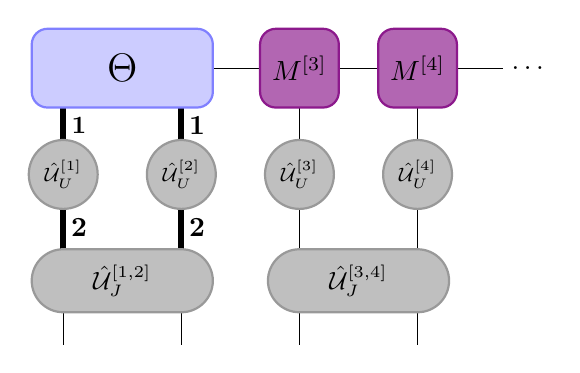
\begin{tikzpicture}[inner sep=1mm]
\def \reldist {1.5};
\def \numb {4};
\def \wid {2.3};
\def \size {1.0};
\def \hi {0.8};
\def \rad {0.4};
\def \vert {1.35};


\foreach \i in  {1,...,\numb} {
	\node[operator] (A\i)
	at (\i * \reldist, 0) {};
	\draw[-] (A\i) -- (\i * \reldist , -2.5*\vert);	
};

\foreach \i in {1,...,3} {
    \pgfmathtruncatemacro{\iplusone}{\i + 1};
    \draw[-] (A\i) -- (A\iplusone);
};


\foreach \i in  {1,...,\numb} {
	\draw[-] (A\i) -- (\i * \reldist , -2.6 *\vert);	
};

\node[operator] (d1) at (1 * \reldist, -\vert) {};
\node[operator] (d2) at (2 * \reldist, -\vert) {};
\node[operator] (dd1) at (1 * \reldist, -2*\vert) {};
\node[operator] (dd2) at (2 * \reldist, -2*\vert) {};


\draw[-,line width=0.8mm] (A1) -- (d1);
\draw[-,line width=0.8mm] (A2) -- (d2);
\draw[-,line width=0.8mm] (dd1) -- (d1);
\draw[-,line width=0.8mm] (dd2) -- (d2);

\foreach \i in  {1,...,\numb} {
	\node[operator,minimum width= \hi cm,minimum height= \hi cm] (op\i)
	at (\i * \reldist, -\vert)
	{\scriptsize $\hat{\mathcal{U}}_{U}^{[ \i ]}$};	
};

\foreach \i in {1,3} {
	\pgfmathtruncatemacro{\j}{\i + 1};
    \node[twositeop, minimum width= \wid cm,minimum height= \hi cm,rounded corners = \rad cm] (top\i)
    at (\reldist*\i + \reldist/2, -2*\vert)
    {\small $\hat{\mathcal{U}}_{J}^{[ \i , \j ]} $};
};


\node (dot2) at (\numb * \reldist + 1.4,0) {$\dots$};
\draw[-] (A\numb) -- (dot2);

\foreach \i in  {3,...,\numb} {
	\node[tensorr,minimum width= \size cm,minimum height= \size cm, rounded corners = 0.2cm] (B\i)
	at (\i * \reldist, 0) {$M^{[ \i ]}$};
};
\node[tensor,minimum width= \wid cm,minimum height= \size cm, rounded corners = 0.2cm] (AA) at (\reldist*1 + \reldist/2, 0) {\Large $\Theta$};



	\node (node1) at (\reldist +0.2, -0.5*\vert -0.05) {\small \textbf{1}};
	\node (node2) at (2*\reldist +0.2, -0.5*\vert -0.05) {\textbf{1}};
	\node (node3) at (\reldist +0.2, -1.5*\vert) {\textbf{2}};
	\node (node4) at (2*\reldist +0.2, -1.5*\vert) {\textbf{2}};	
	
\end{tikzpicture}
\end{subfigure}
\\ % <-- add this
\vspace{5mm}
\begin{subfigure}[b]{0.4\textwidth}
	\caption{}    	
  	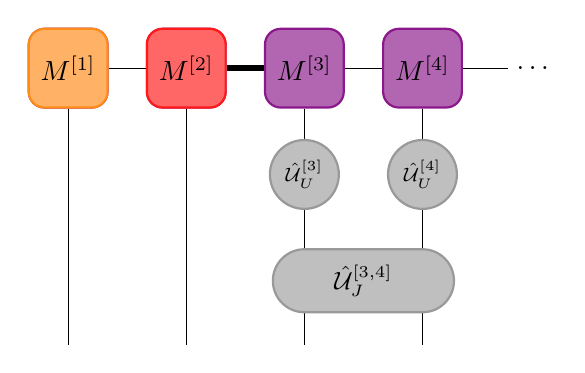
\begin{tikzpicture}[inner sep=1mm]
\def \reldist {1.5};
\def \numb {4};
\def \wid {2.3};
\def \size {1.0};
\def \hi {0.8};
\def \rad {0.4};
\def \vert {1.35};


\foreach \i in  {1,...,\numb} {
	\node[tensorr,minimum width= \size cm,minimum height= \size cm, rounded corners = 0.2cm] (A\i)
	at (\i * \reldist, 0) {$M^{[ \i ]}$};
	\draw[-] (A\i) -- (\i * \reldist , -2.5*\vert);	
};

\foreach \i in {1,...,3} {
    \pgfmathtruncatemacro{\iplusone}{\i + 1};
    \draw[-] (A\i) -- (A\iplusone);
};

\node[tensorl,minimum width= \size cm,minimum height= \size cm, rounded corners = 0.2cm] (L) at (1 * \reldist, 0) {$M^{[1]}$};

\node[tensorc,minimum width= \size cm,minimum height= \size cm, rounded corners = 0.2cm] (C) at (2 * \reldist, 0) {$M^{[2]}$};


\foreach \i in  {1,...,\numb} {
	\draw[-] (A\i) -- (\i * \reldist , -2.6 *\vert);	
};

\draw[-,line width=0.8mm] (A2) -- (A3);

\foreach \i in  {3,...,\numb} {
	\node[operator,minimum width= \hi cm,minimum height= \hi cm] (op\i)
	at (\i * \reldist, -\vert)
	{\scriptsize $\hat{\mathcal{U}}_{U}^{[ \i ]}$};	
};

\foreach \i in {3} {
	\pgfmathtruncatemacro{\j}{\i + 1};
    \node[twositeop, minimum width= \wid cm,minimum height= \hi cm,rounded corners = \rad cm] (top\i)
    at (\reldist*\i + \reldist/2, -2*\vert)
    {\small $\hat{\mathcal{U}}_{J}^{[ \i , \j ]} $};
};


\node (dot2) at (\numb * \reldist + 1.4,0) {$\dots$};
\draw[-] (A\numb) -- (dot2);
	
	
\end{tikzpicture}
\end{subfigure}
\hspace{10mm}
\begin{subfigure}[b]{0.4\textwidth}
	\caption{}  
  	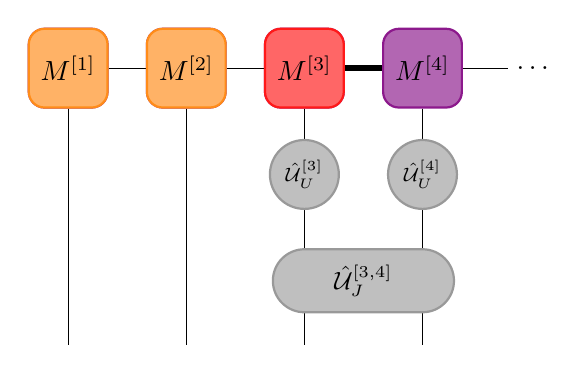
\begin{tikzpicture}[inner sep=1mm]
\def \reldist {1.5};
\def \numb {4};
\def \wid {2.3};
\def \size {1.0};
\def \hi {0.8};
\def \rad {0.4};
\def \vert {1.35};


\foreach \i in  {1,...,\numb} {
	\node[tensorr,minimum width= \size cm,minimum height= \size cm, rounded corners = 0.2cm] (A\i)
	at (\i * \reldist, 0) {$M^{[ \i ]}$};
	\draw[-] (A\i) -- (\i * \reldist , -2.5*\vert);	
};

\foreach \i in {1,...,3} {
    \pgfmathtruncatemacro{\iplusone}{\i + 1};
    \draw[-] (A\i) -- (A\iplusone);
};

\node[tensorl,minimum width= \size cm,minimum height= \size cm, rounded corners = 0.2cm] (L1) at (1 * \reldist, 0) {$M^{[1]}$};

\node[tensorl,minimum width= \size cm,minimum height= \size cm, rounded corners = 0.2cm] (L2) at (2 * \reldist, 0) {$M^{[2]}$};

\node[tensorc,minimum width= \size cm,minimum height= \size cm, rounded corners = 0.2cm] (C) at (3 * \reldist, 0) {$M^{[3]}$};


\foreach \i in  {1,...,\numb} {
	\draw[-] (A\i) -- (\i * \reldist , -2.6 *\vert);	
};

\draw[-,line width=0.8mm] (A3) -- (A4);

\foreach \i in  {3,...,\numb} {
	\node[operator,minimum width= \hi cm,minimum height= \hi cm] (op\i)
	at (\i * \reldist, -\vert)
	{\scriptsize $\hat{\mathcal{U}}_{U}^{[ \i ]}$};	
};

\foreach \i in {3} {
	\pgfmathtruncatemacro{\j}{\i + 1};
    \node[twositeop, minimum width= \wid cm,minimum height= \hi cm,rounded corners = \rad cm] (top\i)
    at (\reldist*\i + \reldist/2, -2*\vert)
    {\small $\hat{\mathcal{U}}_{J}^{[ \i , \j ]} $};
};


\node (dot2) at (\numb * \reldist + 1.4,0) {$\dots$};
\draw[-] (A\numb) -- (dot2);
	
	
\end{tikzpicture}
\end{subfigure}
\caption{\textit{Sequence of contractions for modified tDMRG algorithm during left to right sweep. Step \textbf{(1)}: MPS is centered on site 1. Tensors $M^{[1]}$ and $M^{[2]}$ are contracted. Step \textbf{(2)}: Two-site tensor, $\Theta$, is contracted with operators in numbered sequence. The propagated two-site tensor is split using an SVD in step \textbf{(3)}, followed by a contraction to the right. Lastly, in step \textbf{(4)}, the two-site tensor of $M^{[2]}$ and $M^{[3]}$ is split using another SVD, whereby the center (and thereby the normalisation) is pushed to site 3.}}
\label{fig:TEBDContraction}
\end{figure}
The sequence of contractions of the left-to-right sweep is shown in figure \ref{fig:TEBDContraction}. The MPS is initially centered on the first tensor, while its remaining tensors are right-normalised. By contracting the bonds marked with a bold line shown in step 1 and 2, the operators are efficiently applied to the MPS. In the third step, the two-site tensor, $\Theta$, is split using an SVD, where the bond dimension of the tensors is truncated. This is crucial in order to maintain a reduced dimensionality, which would otherwise result in a significant increase in contraction time. In the final and fourth step, the central cite of the MPS is moved to the start of the next two-site operator through another site merge and subsequent SVD. This step is exactly as in the original tDMRG algorithm. Thereby the normalization of the MPS is "pushed" to the right and contained in a single site, which makes it easy to deal with in the end of the time evolution step.\\
As the center reaches the end of the MPS, the direction of the sweep is reversed. The right-to-left sweep is very similar to the sequence described above. The main difference is in the order of contractions, as the $\hat{\mathcal{U}}_{J}^{[i,i+1]}$-propagator is applied before $\hat{\mathcal{U}}_{U}^{[i]}$. As the sweep, and thereby the central cite, reaches the first site of the MPS, the central site is divided by its norm. Thereby the MPS is normalized and in the same configuration as before the time step. Thus, further propagations can be performed readily.\\ 
Additional precision is achieved when evaluating the control at the beginning and end points of the time interval \cite{Steck2007}. Thus, the left-to-right sweep applies the operator $\hat{\mathcal{U}}_{U(t)}^{[i]} $, while the right-to-left sweep applies $\hat{\mathcal{U}}_{U(t + \Delta t)}^{[i]}$.

The time-evolution algorithm described here shares many traits with one proposed in \cite{Daley2004}, which was tested on the Bose-Hubbard model. The algorithm displayed weak convergence with the maximum bond dimension, $D$, whereby precise results can be obtained using only small bond dimensions. Further improvements to the method were suggested in \cite{Daley2004}, which included utilizing even higher-order expansions of the propagator. By evaluating the parameters of the propagator at specific points in the time interval, $\Delta t$, many algorithmic sweeps can be combined, greatly reducing the computational cost \cite{Yoshida1990,Krech1998}.


\subsubsection{Time complexity of time-evolution algorithms}
\begin{figure}[h!]
    \centering
    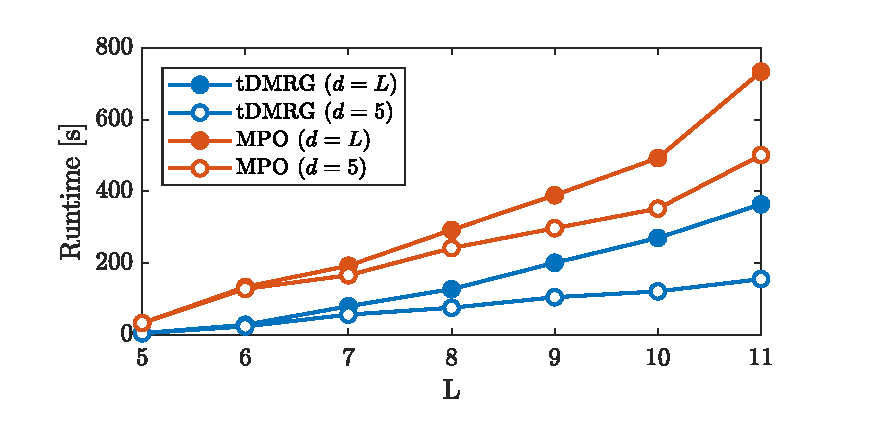
\includegraphics[width=0.7\textwidth]{Figures/CompareRuntime.pdf}
    \caption{\textit{Runtime of performing 100 time steps with two different algorithms in Bose Hubbard system with unit occupancy. The methods are tested on systems with both full and truncated Fock spaces.}}
    \label{fig:CompareRuntime}
\end{figure}
Figure \ref{fig:CompareRuntime} compares runtimes between the modified tDMRG algorithm and the default time evolution method of the ITensor library \cite{ITensor} for various lattice sizes with unit occupancy. The latter method builds the entire propagator as a single layer MPO following \cite{Pollmann2015}, and the resulting MPO is applied to the MPS according to eq. \eqref{eq:optBracketsMPO}. The two methods are tested using local Fock space dimensions, $d$, equal to the length of the lattice, $L$, and set at a constant value of $d = 5$.

In Section \ref{sec:MPO} the cost of applying an MPO to an MPS was given by $\mathcal{O}(L d^2 D_W ^2 D^2)$. Since the tDMRG propagator consists of multiple gates rather than a connected layer, the operator bond dimension, $D_W$, is unit. Thus, the tDMRG algorithm has a cubic scaling with system size. However, a much better scaling can be achieved by truncating the local Hilbert space such that $d$ is kept constant, resulting in a runtime scaling linearly with the system size.
In the case of the Bose Hubbard model, eq. \eqref{BHhamil}, the interaction term scales quadratically with the number of particles at a given site, which causes a huge energy penalty. Thus, for large systems with unit occupation, neglecting contributions from states with a majority of the particles at a single site is a reasonable approximation \cite{Daley2004}.
Therefore, the modified tDMRG algorithm can be applied efficiently to very large systems, if the dimension of the physical index of the MPS is restricted to a reasonable fraction of the number of particles. A similar practice was reported in \cite{Braun2015}, analyzing time-evolution of the Bose-Hubbard model across its phase transition. The study utilized a maximum occupation of 6 was used for systems of sizes $L,N_p = 20 \: \text{to} \: 44$.   
\chapter{Quantum Optimal Control Theory}
The fundamental problem of Quantum Optimal Control Theory is to steer the dynamics of a quantum system in a desired way through external fields \cite{Rice2000,Shapiro2003}. Often, the goal is the transfer from an initial state, $\ket{\psi_0}$, to a desired target-state, $\ket{\psi_{\mathrm{target}}}$. The fields responsible for controlling the dynamics of the system are parametrized by a set of control parameters or functions. Optimal control theory determines the parameters, which lead to the desired dynamics of the system \cite{Werschnik2007}.\\ 
In control problems, the Hamiltonian of the system is given as
\begin{equation}
	\hat{H} =  \hat{H}_0 + \sum_{n = 1}^{m}  \hat{H}_n (u_n(t)) \; ,
	\label{eq:ControlHamiltonians}
\end{equation} 
where $\hat{H}_0$ is an uncontrollable drift, $\hat{H}_n$ are the controllable fields, and $u_n(t)$ are the control functions. A quantum system is completely controllable if every unitary operator, $\hat{U}$, is accessible from the identity operator, $\hat{I}$, via a path $\gamma (t) = \hat{U}(t, t_0)$ satisfying \cite{Schirmer2001}
\begin{equation}
	i \partial_t \hat{U}(t, t_0) = \hat{H} \hat{U}(t, t_0) \; .
\end{equation} 
For an $N$-dimensional Hilbert space, a sufficient condition for complete controllability of a quantum system is that the Lie algebra generated by the Hamiltonians in eq. \eqref{eq:ControlHamiltonians},
\begin{equation}
	L_0 = \mathrm{Lie} \left( i \hat{H}_0, i \hat{H}_1 , \ldots , i \hat{H}_m \right) \; ,
\end{equation}
is of dimension $N^2$ \cite{Ramakrishna1995}.\\
Extending these conditions to infinite-dimensional Hilbert spaces and constrained controls is non-trivial \cite{Huang1983}.


\section{The Gradient-Ascent Pulse Engineering Method - GRAPE} \label{sec:GRAPE}
The control problem presented in this thesis is steering the system from an initial state in the superfluid phase to a target-state in the Mott-Insulator phase. This is achieved by varying the lattice depth, which therefore can be considered the control parameter.\\
The optimal control problem can be stated as follows: 
Suppose the system is initially described by the state $\ket{\psi_0} = \ket{\psi (0)}$, and the potential is varied in the time interval $[ 0 , T]$. The goal is finding the set of control parameters, $\boldsymbol{u}(t)$, which brings the initial state as close as possible to the target-state, $\ket{\psi_{\mathrm{target}}}$. This is expressed in terms of a cost function
\begin{equation}
	J_T = \frac{1}{2} \left( 1-|\braket{\psi_{\mathrm{target}} | \psi (T)}|^2 \right) \; ,
	\label{eq:infidelityCost}
\end{equation}
which is given as half the infidelity between the target and the state at $t=T$. The cost function becomes zero, when the terminal state matches the target state up to an arbitrary phase. Hence, the optimal control problem can be formulated as a minimization problem of eq. \eqref{eq:infidelityCost} \cite{Jager2014}.\\
Large variations in the control parameter is often hard to achieve experimentally. Therefore, an extra term is added to the cost function, which penalizes strong variations in the control. The new cost function reads
\begin{equation}
	J = J_T + J_R = J_T + \frac{\gamma}{2} \sum_{n=1}^{m} \int_{0}^{T} \left( \pdv{u_n}{t} \right)^2 \mathrm{d}t \; ,
	\label{eq:grapeCost}
\end{equation}
where $\gamma$ weighs the relative importance between matching states and smoothness of the control \cite{Jager2014}. As the state transfer is considered the highest priority, $\gamma \ll 1$ such that $J_T$ dominates the cost function of eq. \eqref{eq:grapeCost}.\\

A powerful way of performing optimal control is the Gradient-Ascent Pulse Engineering (GRAPE) method. Through GRAPE, the gradient of the cost function \eqref{eq:grapeCost} can be evaluated and used to update the existing set of controls \cite{Khaneja2005}. Thereby, one achieves an optimization of the cost function.\\
The gradient of the cost function can be derived in multiple ways. A common method is introducing a Lagrange multiplier \cite{Hohenester2007, Winckel2008, BECcontrol}, which forces the dynamics to obey the Schrödinger equations. This method considers the states and the control as continuous functions, which must be discretized after the derivation of the gradient for numerical purposes. However, postponing the discretization until the very last step causes a loss of accuracy, as a series of higher order corrections due to the discretization are lost.
Here, an alternative derivation following \cite{Khaneja2005, deFouquieres2011} is presented in which the discretization is introduced immediately. \\
Assume the transfer time, $T$, is discretized in steps of $\Delta t = T/N$. Subjecting the control to a similar discretized yields
\begin{equation}
	u_n = \left( u_n (t_1) , \ldots , u_n (t_N)  \right)  \; .
\end{equation}
The time-evolution of the system during the time step $j$ is given by the propagator
\begin{equation}
	\hat{\mathcal{U}}_j \equiv \hat{\mathcal{U}} (u(t_j)) = \exp \bigg\{ -i \left(  \sum_{n = 1}^{m}  \hat{H}_n (u_n(t_j))  \right) \Delta t \bigg\} \; . 
\end{equation} 
Thereby, the cost function \eqref{eq:grapeCost} becomes
\begin{equation}
	J = \frac{1}{2} \left( 1 - |\braket{\psi_{\mathrm{target}} | \prod_{j = 1}^{N} \hat{\mathcal{U}}_j | \psi (0)}|^2 \right) + \frac{\gamma}{2} \sum_{n = 1}^{m} \sum_{j = 1}^{N-1} \left( \frac{\Delta u_n (t_j)}{\Delta t} \right)^2 \Delta t \; ,
	\label{eq:discreteCost}
\end{equation}
where $\Delta u_n (t_j) =  u_n (t_{j+1}) - u_n (t_j)$. The full gradient of the cost, $\nabla J(\boldsymbol{u})$, is a vector of partial derivatives $\frac{\partial J(\boldsymbol{u})}{\partial u_n (t_j)}$, which can be derived analytically.\\
First, consider the derivative of the regularization
\begin{align}
	\frac{\partial J_R}{\partial u_n (t_j)} &= \frac{\gamma}{2} \left( 2 \frac{u_n (t_j) - u_n (t_{j-1})}{\Delta t^2} - 2 \frac{u_n (t_{j+1}) - u_n (t_j)}{\Delta t^2} \right) \Delta t \nonumber \\
	&= \frac{\gamma}{\Delta t} \left( 2 u_n (t_j) - u_n (t_{j+1}) - u_n (t_{j-1}) \right) \; . \label{eq:regularizationGrad}
\end{align}
The part of the gradient related to the regularization depends only on the control, whereby it can be calculated without considering the state of the system.\\ 
Next, consider the derivative of $J_T$. Defining the transfer probability amplitude $\tau \equiv \braket{\psi_{\mathrm{target}} | \psi (T)}$, the derivative of the final infidelity with respect to the control can be written as 
\begin{equation}
	\frac{\partial J_T}{\partial u_n (t_j)} = - \frac{1}{2} \frac{\partial}{\partial u_n (t_j)}  \tau^* \tau   = - \Re \left( \tau^* \frac{\partial \tau}{\partial u_n (t_j)} \right) \; .
	\label{eq:dJTdu}
\end{equation}
From eq. \eqref{eq:dJTdu} it is evident that the derivative of the infidelity depends only on the derivative of the transfer probability amplitude, $\frac{\partial \tau}{\partial u_n (t_j)}$. This derivative can be rewritten as
\begin{align}
	\frac{\partial \tau}{\partial u_n (t_j)} &= \frac{\partial }{\partial u_n (t_j)} \Braket{\psi_{\mathrm{target}} | \prod_{j = 1}^{N} \hat{\mathcal{U}}_j | \psi (0)} \nonumber \\
	&= \Braket{\psi_{\mathrm{target}} | \hat{\mathcal{U}}_N \ldots \hat{\mathcal{U}}_{j+1} \frac{\partial \hat{\mathcal{U}}_{j}}{\partial u_n (t_j)} \hat{\mathcal{U}}_{j-1} \ldots \hat{\mathcal{U}}_{1} | \psi (0)}
	\label{eq:dcdu}
\end{align}
Multiplying eq. \eqref{eq:dcdu} with $\tau^*$ to recreate the result of eq. \eqref{eq:dJTdu} yields
\begin{align}
	\tau^* \frac{\partial \tau}{\partial u_n (t_j)} &=  \braket{\psi(T) | \psi_{\mathrm{target}}} \Braket{\psi_{\mathrm{target}} | \prod_{j' = j +1}^{N} \hat{\mathcal{U}}_{j '} \frac{\partial \hat{\mathcal{U}}_{j}}{\partial u_n (t_j)} \prod_{j' = 1}^{ j-1} \hat{\mathcal{U}}_{j '} | \psi (0)} \\
	&= i \Braket{\chi (T) | \prod_{j' = j +1}^{M} \hat{\mathcal{U}}_{j '} \frac{\partial \hat{\mathcal{U}}_{j}}{\partial u_n (t_j)} \prod_{j' = 1}^{ j-1} \hat{\mathcal{U}}_{j '} | \psi (0)} \\
	&= i \Braket{\chi (t_j) |  \frac{\partial \hat{\mathcal{U}}_{j}}{\partial u_n (t_j)} | \psi (t_{j-1})} \; ,
	\label{eq:gradientForBack}
\end{align}
where $\ket{\chi (T)} \equiv i \ket{\psi_{\mathrm{target}}} \braket{\psi_{\mathrm{target}} | \psi (T)}$ is the projection of the final state unto the target state. Notice how in eq. \eqref{eq:gradientForBack} the state $\ket{\chi (T)}$ has been propagated backwards in time.\\ 
The derivative of the propagator, $\hat{\mathcal{U}}_{j}$, is non-trivial, due to possible non-commutativity between the Hamiltonian and its derivative. This results in a series of higher order corrections to the derivative of propagator.
Expanding the propagator as a Taylor series before taking the derivative gives
\begin{align}
	\frac{\partial \hat{\mathcal{U}}_{j}}{\partial u_n (t_j)} &= \frac{\partial}{\partial u_n (t_j)}  \exp \left( -i \hat{H} \Delta t \right) \nonumber \\
	&= \sum_{p = 0}^{\infty} \frac{( -i \Delta t  )^p}{p!} \frac{\partial \hat{H}^p}{\partial u_n (t_j)} \; .  
	\label{eq:derivTaylorExp}
\end{align}
As mentioned before the Hamiltonian may not commute with its derivative. Therefore, one must be careful when taking the derivative of $\hat{H}^p$. Retaining the ordering of the operators while taking the derivative yields
\begin{align}
	\frac{\partial \hat{\mathcal{U}}_{j}}{\partial u_n (t_j)} &= \sum_{p=1}^{\infty} \frac{ \left( -i \Delta t \right) ^p }{p!} \sum_{q=0}^{p-1} \hat{H}^q \frac{\partial \hat{H}}{\partial u_n (j)} \hat{H}^{p-q-1} \nonumber \\
	&= \sum_{p=0}^{\infty} \sum_{q=0}^{\infty} \frac{A^p B A^q}{(p+q+1)!} \; , \label{eq:derivTaylorExp2}
\end{align} 
where $A \equiv -i \hat{H} \Delta t$ and $B \equiv -i \partial \hat{H}/\partial u_n (t_j) \Delta t$ have been defined for notational convenience. Through the standard relations of the gamma function, $\Gamma (z)$, one can derive the identity
\begin{equation}
	\frac{1}{(p+q+1)!} = \frac{1}{p! q !} \int_{0}^{1} (1-\alpha)^p \alpha^q \mathrm{d}\alpha \; .
\end{equation}
Thereby eq. \eqref{eq:derivTaylorExp2} can be expressed as
\begin{align}
	\frac{\partial \hat{\mathcal{U}}_{j}}{\partial u_n (t_j)} &= \sum_{p=0}^{\infty} \sum_{q=0}^{\infty} \frac{A^p B A^q}{p! q !}  \int_{0}^{1} (1-\alpha)^p \alpha^q \mathrm{d}\alpha \nonumber \\
	&= \int_{0}^{1} \sum_{p=0}^{\infty} \sum_{q=0}^{\infty} \frac{(A (1- \alpha))^p}{p!} B \frac{(A \alpha)^q}{q!}  \mathrm{d}\alpha \nonumber \\
	&= \int_{0}^{1} e^{ (1- \alpha) A} B e^{ \alpha A} \mathrm{d}\alpha \nonumber \\
	 &= e^A \int_{0}^{1} e^{ - \alpha A} B e^{ \alpha A} \mathrm{d}\alpha \; , \label{eq:eq:derivTaylorExp3}
\end{align}
where the expansion of the exponential function has been used to eliminate the sums. Although eq. \eqref{eq:eq:derivTaylorExp3} looks rather simple, evaluating the integral in its current form is a fairly hard task. Instead, the integral can be explicitly solved by applying the Baker–Campbell–Hausdorff expansion 
\begin{equation}
	e^X Y e^{-X} = \sum_{k = 0}^{\infty} \frac{ [ X,Y  ]_k }{k!} = Y + [ X,Y  ] + \frac{1}{2!} [ X , [ X,Y  ]] + \frac{1}{3!} [X, [ X , [ X,Y  ]]  ] + ...
\end{equation}
where $[ X , Y ]_k = [ X ,[ X , Y]]_{k-1}$ and $[X,Y]_0 = Y$ is the definition of the recursive commutator \cite{Wilcox1967}. Thus, eq. \eqref{eq:eq:derivTaylorExp3} reads
\begin{align}
	\frac{\partial \hat{\mathcal{U}}_{j}}{\partial u_n (t_j)} &=  e^A \int_{0}^{1} \sum_{k = 0}^{\infty } \alpha^{k} \frac{(-1)^k}{k!} [ A,B  ]_k \mathrm{d}\alpha \nonumber \\
	&= e^A  \sum_{k = 0}^{\infty }  \frac{(-1)^k}{(k+1)!} [ A,B  ]_k \; .
\end{align}
Inserting this final expression for the derivative of the propagator into eq. \eqref{eq:dJTdu}, one finds the exact derivative of the infidelity 
\begin{align}
\frac{\partial J_T}{\partial u_n (t_j)} &=  - \Re  \Braket{\chi (t_j) | i e^{-i \hat{H} \Delta t}  \sum_{k = 0}^{\infty }  \frac{(-1)^k}{(k+1)!} \left[ -i \hat{H} \Delta t , -i \frac{\partial \hat{H}}{\partial u_n (t_j)} \Delta t  \right]_k | \psi (t_{j-1})}  \nonumber \\
	&=  - \Re  \Braket{\chi (t_{j-1}) | \sum_{k = 0}^{\infty }  \frac{i^{k} \Delta t^{k+1}}{(k+1)!} \left[ \hat{H} , \frac{\partial \hat{H}}{\partial u_n (t_j)}  \right]_k | \psi (t_{j-1})}  \; . \label{eq:higherOrderGradient}
\end{align}
For small time-steps the higher order corrections can be neglected, however, choosing a larger time-step reduces the run-time of the time-evolution, which is critical when describing many-body systems. Therefore, when using large time-steps, higher-order correlations should be included to preserve accuracy. Computing the higher order corrections can be done efficiently by analytically deriving the commutators beforehand. In section \ref{sec:modTMDRG} an alternative propagator is constructed using the Suzuki-Trotter expansion, which causes the gradient to be exact to zeroth order.\\
Finally, combining the derivatives of eq. \eqref{eq:regularizationGrad} and \eqref{eq:higherOrderGradient} produces the entries of the gradient vector for the cost function
\begin{align}
	\frac{\partial J (\boldsymbol{u})}{\partial u_n (t_j)}  &= - \Re \Braket{\chi (t_{j-1}) | \left( i \frac{\partial \hat{H}}{\partial u_n (t_j)} \Delta t + \mathrm{h.o.} \right)  | \psi (t_{j-1})}  \nonumber \\
	& \quad + \frac{\gamma}{\Delta t} \left( 2 u_n (t_j) - u_n (t_{j+1}) - u_n (t_{j-1}) \right) \; .
	\label{eq:costGradient}
\end{align}
Here $\mathrm{h.o.}$ denotes all higher order terms ($k > 0$).\\ 
Through the analytically derived gradient, the cost can be iteratively updated using gradient-based optimization methods until a desired threshold is reached. This forms the framework of the Gradient-Ascent Pulse Engineering (GRAPE) algorithm \cite{Khaneja2005}.
\begin{algorithm}
\begin{algorithmic}
\caption{GRAPE Algorithm}
\State Choose initial control $\boldsymbol{u}^{(1)}$.
\While{$ J > J_{\mathrm{threshold}}$}
	\State Calculate $\ket{\psi (t_k)} = \prod_{j=1}^{k} \hat{\mathcal{U}}_j \ket{\psi (0)}$ for $k = 1 \ldots N$.
	\State Calculate $\ket{\chi (t_k)} = \prod_{j=N}^{k} \hat{\mathcal{U}}_{j}^{\dag} \ket{\chi (T)}$ for $k = N \ldots 1$. 
	\State Evaluate $\frac{\partial J}{\partial u_n (t_k)}$ for $k = 1 \ldots N$ and $n = 1 \ldots m$ according to eq. \eqref{eq:costGradient}.
	\State Update controls using gradient such that $J^{(i + 1)} < J^{(i)}$. 
\EndWhile
\end{algorithmic}
\end{algorithm}
The cost is minimized under the initial and terminal condition
\begin{align}
	\boldsymbol{u}(0) &= \text{fixed value} \label{eq:firstBound} \\
	\boldsymbol{u}(T) &= \text{fixed value} \\
	\ket{\psi (0)} &= \ket{\psi_0} \\
	\ket{\chi (T)} &= i \ket{\psi_{\mathrm{target}}} \braket{\psi_{\mathrm{target}} | \psi (T)} \; .  \label{eq:lastBound}
\end{align}
Although the starting guess of the control, $\boldsymbol{u}^{(1)}$, can be completely random, both faster convergence and lower convergence value is achieved by choosing a good starting seed. Clearly, there is no guarantee that the algorithm will converge to the global optimum, as it is based on a gradient ascent procedure \cite{Khaneja2005}. Nevertheless, the algorithm can be made to search a large portion of the parameter space by executing it multiple time for various seeds.  

In practice, the GRAPE algorithm requires a lot of computer memory, as the gradient of the cost requires the inner product of the states $\ket{\psi}$ and $\ket{\chi}$ at all times, $t_k$. The two states cannot be time-evolved simultaneously, as $\ket{\chi}$ is derived from the final state. To efficiently evaluate the gradient, the state $\ket{\psi}$ must be stored at each time-step, while entries of the gradient \eqref{eq:costGradient} are calculated at each step of the back-propagation of $\ket{\chi}$. Thus, a total of $N$ states must be kept in each iteration of the GRAPE algorithm. For complex many-body systems this may become an issue, as tensor-network descriptions of states (described in chapter \ref{chap:MPS}) require a lot of storage. A possible workaround is proposed in \cite{Mennemann2015}, which involves calculating the final state, $\ket{\psi (T)}$, without storing the state at every step. Subsequently, the two states $\ket{\psi (T)}$ and $\ket{\chi (T)}$ are both propagated backwards simultaneously, and the elements of the gradient \eqref{eq:costGradient} are calculated at each step. This eliminates the need for storing a large amount of information, as a maximum of two states will be kept in the memory at a time. However, this memory-preserving version of the GRAPE algorithm requires an additional time-evolution of $\ket{\psi}$ in each iteration resulting in an increased runtime.


\subsection{Gradient of Suzuki-Trotter Propagator}
In section \ref{sec:GRAPE} the derivative of the cost function with regards to the control was derived for a general propagator. However, expanding the propagator using the Suzuki-Trotter expansion while having a diagonal control Hamiltonian causes all higher order contributions to the gradient to drop out. Instead, the precision of the gradient is solely determined by the order of the expansion.\\
Consider the gradient entries for the cost function derived in section \ref{sec:GRAPE}
\begin{equation}
	\frac{\partial J}{\partial u_n (t_j)} = - \Re \Braket{\chi (t_j) | i \frac{ \partial \hat{\mathcal{U}}_{j}}{\partial u_n (t_j)} | \psi (t_{j-1})} \; ,
\end{equation}
where the derivative of a general propagator with respect to the control is given by
\begin{equation}
	\frac{\partial \hat{\mathcal{U}}_{j}}{\partial u_n (t_j)} = e^{-i \hat{H} (u_n (t_j)) \Delta t}  \sum_{k = 0}^{\infty }  \frac{i^{k-1} \Delta t^{k+1}}{(k+1)!} \left[ \hat{H} (u_n (t_j)) , \frac{\partial \hat{H} (u_n (t_j))}{\partial u_n (t_j)}  \right]_k \;.
\end{equation}
The algorithm in this instance employs a Suzuki-Trotter expansion of the propagator while considering the control at both start and end of the step. For cleaner notation the Hamiltonian, which in this case is the Bose-Hubbard Hamiltonian of eq. \eqref{BHhamil}, will be parametrized as $\hat{H}(U(t_j)) \equiv \hat{H}_J + U(t_j) \hat{H}_U$. Note, that the control in this instance is the interaction strength, $u_n (t_j) \equiv U (t_j)$. Thus, the full propagator reads
\begin{equation}
	\hat{\mathcal{U}}_{j}^{\mathrm{ST}} = \exp \left( -i U(t_j) \hat{H}_U \Delta t /2 \right) \exp \left( -i \hat{H}_J \Delta t \right) \exp \left( -i  U(t_{j-1}) \hat{H}_U  \Delta t /2 \right)  \equiv \hat{\mathcal{U}}_{j}^{U} \hat{\mathcal{U}}_{j}^{J} \hat{\mathcal{U}}_{j-1}^{U} \; .
\end{equation}
Since the control at times $t_j$ and $t_{j-1}$ contribute to $\hat{\mathcal{U}}_{j}^{\mathrm{ST}}$, the elements of the cost gradient are
\begin{equation}
	\frac{\partial J}{\partial U (t_j)} = - \Re \Braket{\chi (t_j) | i  \frac{\partial \hat{\mathcal{U}}_{j}^{\mathrm{ST}}}{\partial U (t_j)} | \psi (t_{j-1})} - \Re \Braket{\chi (t_{j+1}) | i \frac{ \partial \hat{\mathcal{U}}_{j+1}^{\mathrm{ST}}}{\partial U (t_j)} | \psi (t_{j})} \; . \label{eq:STcostderiv}
\end{equation}
Further examining the derivative of the first propagator reveals
\begin{align}
	\frac{\partial \hat{\mathcal{U}}_{j}^{\mathrm{ST}}}{\partial U (t_j)} &=  \frac{\partial \hat{\mathcal{U}}_{j}^{U}}{\partial U (t_j)} \hat{\mathcal{U}}_{j}^{J} \hat{\mathcal{U}}_{j-1}^{U} \nonumber \\
	&=  \exp \left( -i U (t_j) \hat{H}_U  \Delta t /2 \right)  \sum_{k = 0}^{\infty }  \frac{i^{k-1} \Delta t^{k+1}}{(k+1)!} \left[ U (t_j) \hat{H}_U  ,  \hat{H}_U \right]_k \hat{\mathcal{U}}_{j}^{J} \hat{\mathcal{U}}_{j-1}^{U} \nonumber \\
	&= \left( -i \hat{H}_U \Delta t /2 \right) \exp \left( -i U(t_j) \hat{H}_U  \Delta t /2 \right)   \hat{\mathcal{U}}_{j}^{J} \hat{\mathcal{U}}_{j-1}^{U} \nonumber \\
	&= \left( -i \hat{H}_U \Delta t /2 \right) \hat{\mathcal{U}}_{j}^{\mathrm{ST}} \; . \label{eq:STpropderiv1}
\end{align}
Since $\hat{H}_U$ is diagonal, the following relation apply for the recursive commutator 
\begin{equation}
	\left[ U (t_j) \hat{H}_U  ,  \hat{H}_U \right]_k =  
	\begin{cases}
    	\hat{H}_U, & \text{if $k = 0$}.\\
    	0, & \text{otherwise}.
  	\end{cases} \; ,
\end{equation}  
which causes all higher-order contributions to the derivative of the propagator to drop out.\\
Likewise, the derivative of the second propagator is
\begin{equation}
	\frac{\partial \hat{\mathcal{U}}_{j+1}^{\mathrm{ST}}}{\partial u_n (j)} =  \hat{\mathcal{U}}_{j+1}^{\mathrm{ST}} \left( -i \hat{H}_U \Delta t /2 \right) \; . \label{eq:STpropderiv2}
\end{equation}
Inserting the derivatives of eq. \eqref{eq:STpropderiv1} and \eqref{eq:STpropderiv2} into the derivative of the cost (eq. \eqref{eq:STcostderiv}) yields
\begin{align}
	\frac{\partial J}{\partial U (t_j)} &= - \Re \Braket{\chi (t_j) |   \left(  \hat{H}_U \Delta t /2 \right) \hat{\mathcal{U}}_{j}^{\mathrm{ST}} | \psi (t_{j-1})} - \Re \Braket{\chi (t_{j+1}) |  \hat{\mathcal{U}}_{j+1}^{\mathrm{ST}} \left(  \hat{H}_U \Delta t /2 \right) | \psi (t_{j})} \nonumber \\
	&= - \Re \Braket{\chi (t_j) |  \hat{H}_U \Delta t /2  | \psi (t_{j})} - \Re \Braket{\chi (t_{j}) |  \hat{H}_U \Delta t /2   | \psi (t_{j})} \nonumber \\
	&= - \Re \Braket{\chi (t_j) | \hat{H}_U \Delta t | \psi (t_{j})} \; . \label{eq:STcostgrad}
\end{align}  
Thus, the combination of the Suzuki-Trotter expansion and a diagonal control Hamiltonian eliminates all higher order contributions to the gradient. Thereby, the gradient of the cost is exact up to the order of the expansion.
\begin{figure}[!h]
    \centering
    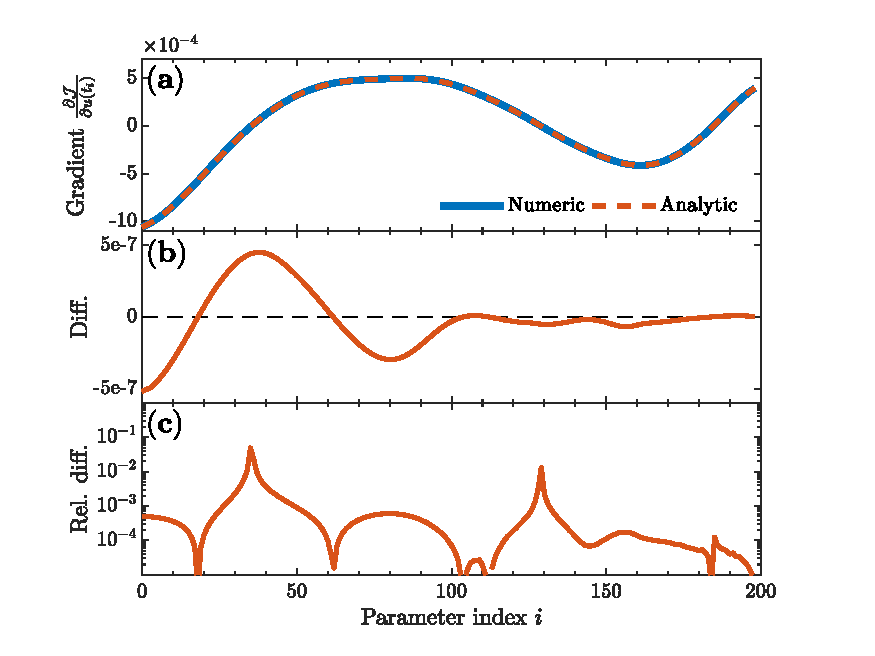
\includegraphics[width=0.8\textwidth]{Figures/CompareGradientsGRAPE.pdf}
    \caption{\textit{\textbf{(a)}: Numerical gradient along with gradient calculated via eq. \eqref{eq:STcostgrad}. \textbf{(b)}: Difference between the two gradients. \textbf{(c)}: Absolute relative difference between the two gradients.}}
    \label{fig:CompareGradientsGRAPE}
\end{figure}
A comparison between a numerically calculated gradient and the analytically derived gradient of eq. \eqref{eq:STcostgrad} can be seen in figure \ref{fig:CompareGradientsGRAPE}. The difference between the two gradients is largest at the beginning of the sequence, due to the accumulated error from the time evolution of $\ket{\chi (0)}$, which is derived from two time evolutions over the entire duration.


\section{Interior Point Methods} \label{sec:IntPoint}

The GRAPE method formulates the control problem as the minimization of the cost function \eqref{eq:grapeCost} while providing the derivative of the cost with respect to the control functions \eqref{eq:costGradient}. Thus, the optimal control can be found using well established methods from mathematical optimization theory. Generally, control problems are very hard to solve, as they are highly non-linear, have many control parameters (even when parametrized), and are often subjected to a series of constraints. An example of the latter can be seen when considering optimizations within the Bose-Hubbard model, as the model is valid only within the tight-binding limit. Thus, the control problem will be subject to the non-linear constraint
\begin{equation}
	 V_{0}^{\mathrm{min}} \leq c (u(t)) \leq V_{0}^{\mathrm{max}} \; ,
\end{equation}
where $c (u)$ is some constraint function dependent on the parameterization of the problem.\\
Interior point methods are currently considered some of the most powerful algorithms for large-scale non-linear programming. The methods update the control parameters using the derivatives of the cost function via Newtons method, from which they differ in many ways in order to accommodate the constraints. Interior point methods approach the solution from within the feasible region as opposed to other methods like Nelder-Mead, hence the name \textit{interior}. In addition, they provide efficient performance while having better theoretical properties than the standard simplex method \cite{wright}.\\

In this section the simplest version of non-linear interior point method is derived, however, many variants of the method exists with respect to update strategies, line searches, handling non-convexity and more.\\
Consider the general minimization problem of some objective $f(x)$
\begin{subequations}	
 \begin{align}
	\min_{x } 			\quad & f(x) 			\\
	\text{subject to} 	\quad & g(x) = 0  		\\ 
						   	  & h(x) \geq 0 	\; ,
\end{align}
\label{eq:GeneralOptProblem}
\end{subequations}
where $g(x)$ and $h(x)$ are a set of equality and inequality constraints. The Lagrangian for the general constrained optimization problem \eqref{eq:GeneralOptProblem} is defined as
\begin{equation}
	\mathcal{L}(x,\lambda,\zeta) = f(x) - \lambda^T g(x) - \zeta^T h(x)  \; ,
\end{equation}
where $\lambda$ and $\zeta$ are vectors of Lagrange multipliers of the equality and inequality constraints respectively. Thus, one must find a point $(x^*,\lambda^*,\zeta^*)$ minimizing the objective function while satisfying the constraints.

\subsection{Duality}
Duality theory describes how an alternative \textit{dual} problem can be derived from the original \textit{primal} problem and how the two problems are related. Thus, the dual problem can be regarded as a different perspective of the original problem. Much information regarding the original problem can be inferred from the solution of its dual, hence many non-linear optimization algorithms solve primal-dual problems.\\
The dual function is defined as
\begin{equation}
	q (\lambda , \zeta) = \inf_{x} \mathcal{L} (x,\lambda,\zeta) \; ,
\end{equation}
where the infimum is required to exist and be finite. Note how the Lagrange multipliers of the primal problem are the optimization parameters of its dual. The dual function always satisfies the condition of \textit{weak duality}
\begin{equation}
	f(x^*) \geq q (\lambda^* , \zeta^*) \; ,
	\label{eq:WeakDuality}
\end{equation} 
whereby it provides a lower bound on the solution of \eqref{eq:GeneralOptProblem}. In order for the direction of the inequality constraint to remain the same, it is necessary that all the inequality Lagrange multipliers fulfill $\zeta_i \geq 0$. This requirement can be considered a constraint of the dual, since the Lagrange multipliers are the variables of the dual function. Thus, the dual problem is defined as
\begin{subequations}	
 \begin{align}
	\max_{\lambda , \zeta} 	\quad 	& q(\lambda , \zeta) 				\\
	\text{subject to} 		\quad 	& \zeta \geq 0  			\; .
\end{align}
\label{eq:GeneralDualProblem}
\end{subequations}
A very nice property of the dual problem is that it is always convex regardless of $f(x)$. Thus, the dual problem is often easier to solve than the primal. Furthermore, the solutions of the dual problem are the optimal Lagrange multipliers of the original problem, which would otherwise be very hard to find.
Another useful feature in duality theory is the \textit{duality gap}, which is given by the difference between the primal and dual function, $f(x) - q(\lambda , \zeta )$. Considering the condition of weak duality \eqref{eq:WeakDuality}, the duality gap implies that
\begin{equation}
	f(x) - f(x^*) \leq f(x) - g(\lambda , \zeta) \; ,
	\label{eq:DualityGapIneq}
\end{equation}
whereby $x$ is primal optimal and $\lambda , \zeta$ are dual optimal, if the duality gap is zero. Thus, eq. \eqref{eq:DualityGapIneq} can be used as a stopping criteria for optimization algorithms, as the duality gap will tend towards zero for $x \to x^*$.


\subsection{Karush–Kuhn–Tucker Conditions}
The Karush–Kuhn–Tucker (KKT) conditions are a set of first-order necessary conditions for a point $(x^*,\lambda^*,\zeta^*)$ being an optimum. They only consider properties of the gradient of the objective and constraint function, hence the \textit{first-order} label. The KKT conditions are very important in optimization theory, as many algorithms (including interior point methods) can be interpreted as solving a set of equations directly derived from the conditions.    

\begin{theorem}
	Let the active constraints be all the equality constraints along with the set of inequality constraints fulfilling $h(x) = 0$ for some feasible $x$. Suppose that $x^*$ is a local solution of \eqref{eq:GeneralOptProblem} and the gradients of the active constraints are linearly independent at $x^*$. Then Lagrange multiplier vectors $\lambda$ and $\zeta$ exists, such that the following conditions are satisfied at $(x^*,\lambda^*,\zeta^*)$ \cite{wright}
\begin{subequations}	
\begin{align}
\nabla_x \mathcal{L}(x^*,\lambda^*,\zeta^*) &= 0 \; ,  	\\
g(x^*) &= 0 \; ,  \label{eq:KKTprimal1}					\\
h(x^*) &\geq 0 \; ,  \label{eq:KKTprimal2}				\\
\zeta^*  &\geq 0 \; , \label{eq:KKTdual}					\\ 
\zeta_{i}^* h_i (x^*) &= 0 \; , \quad \mathrm{for} \; i = 1 , \ldots , m \label{eq:KKTslack}
\end{align}
\label{eq:KKTconditions}
\end{subequations}	  
\end{theorem}
The first condition is called the \textit{stationary condition} and simply states that the point $(x^*,\lambda^*,\zeta^*)$ must be stationary point, which is a general requirement for a point to be considered an optimum. Next, the conditions \eqref{eq:KKTprimal1} and \eqref{eq:KKTprimal2} are the \textit{primal feasibility}, which coincide with the constraints originally stated in the problem \eqref{eq:GeneralOptProblem}. The following condition \eqref{eq:KKTdual} is the \textit{duality feasibility}, which is a constraint of the dual problem \eqref{eq:GeneralDualProblem} discussed earlier.
The last condition is the \textit{complementary slackness}, which arises from the requirement $\zeta^{*T} h(x^*) = 0$. The two previous conditions state that $\zeta_{i}^{*} h_i(x^*) \geq 0$, whereby the condition \eqref{eq:KKTslack} is needed for each inequality constraint.\\
If the point $(x^*,\lambda^*,\zeta^*)$ satisfies all the KKT conditions, then the point is the solution to the primal-dual problem.


\subsection{Basic Primal-Dual Interior Point Algorithm}
Interior point methods solve a set of equations derived directly from the KKT conditions using Newtons method. However, Newtons method is in general not compatible with inequality constraints, hence the original problem \eqref{eq:GeneralOptProblem} must be reformulated. Instead, the interior point methods solve barrier problems of the form 
\begin{subequations}	
 \begin{align}
	\min_{x,s} 			\quad & f(x) - \mu \sum_{i = 1}^{m} \log s_i \\
	\text{subject to} 	\quad & g(x) = 0  		\\ 
						   	  & h(x) - s  = 0 	\; ,
\end{align}
\label{eq:BarrierProblem}
\end{subequations}
where $\mu$ is the positive barrier parameter, and $s$ is a vector of slack variables, which transforms the inequality constraint into an equality at the cost of adding additional optimization variables. In order to ensure the direction of the inequality constraint, it is a requirement that $s \geq 0$. While this is an inequality constraint itself, it is enforced via the logarithmic barrier term, which diverges as any component of $s$ approaches zero. Furthermore, the barrier term does not add much complexity to the problem, as it convex and twice differentiable.\\
The step direction towards the KKT-point can be found through Newtons method, however, often one can only take a small step before violating the constraints, hence the pure Newton direction is dubbed the \textit{affine scaling direction}. The barrier approach consists of finding solutions of the barrier problem \eqref{eq:BarrierProblem} for a sequence of barrier parameters $\{ \mu_k \}$ converging to zero. Several strategies exist for updating the barrier parameters, however, their common goal is to bias the step direction of the algorithm, such that the longest possible steps can be taken. The solutions of the barrier subproblems can be denoted $(x(\mu),s(\mu), \lambda(\mu),\zeta(\mu))$, and the trajectory of these points is known as the \textit{primal-dual central path}, which converges to $(x^*,s^*, \lambda^*,\zeta^*)$ as $\mu \to 0$.\\

The KKT conditions of the barrier problem \eqref{eq:BarrierProblem} can be expressed in a single mapping 
\begin{equation}
	F \equiv 
	\begin{bmatrix}
  \nabla_x f(x) - A_{g}^{T}(x) \lambda  - A_{h}^{T}(x) \zeta \\
  S \zeta - \mu e \\
  g(x)		\\
  h(x) - s 
  \end{bmatrix}
  = 0 \; ,
  \label{eq:BarrierKKTmap}
\end{equation}
where $A_g (x)$ and $A_h (x)$ are the Jacobian matrices of the constraint functions $g(x)$ and $h(x)$. Additionally, $S$ and $Z$ are defined as diagonal matrices with entries given by the vectors $s$ and $\zeta$, while $e = (1 ,1 , \ldots , 1 )^T$. Note how the introduction of the slack variables and the barrier term has modified the original KKT conditions \eqref{eq:KKTconditions}. Transforming the constraints has removed the need for the duality feasibility \eqref{eq:KKTdual}, while barrier term "relaxes" the complementary slackness \eqref{eq:KKTslack}, whose original form is recovered as $\mu \to 0$.\\
Applying Newtons method to the set of non-linear equations \eqref{eq:BarrierKKTmap} yields
\begin{equation}
  \begin{bmatrix}
  \nabla_{xx} \mathcal{L} 	& 0 	& -A_{g}^{T}(x)	& -A_{h}^{T}(x)	\\
  0 						& Z 	& 0 			& S 			\\
  A_{g}(x) 					& 0 	& 0 			& 0				\\
  A_{h}(x) 					& -I	& 0				& 0				 
  \end{bmatrix}  
  \begin{bmatrix}
  p_x \\ p_s \\ p_{\lambda} \\ p_{\zeta} 
  \end{bmatrix}
  = - F
  \label{eq:ConNewtonMethod}
\end{equation}
where $p = ( p_x , p_s , p_{\lambda} , p_{\zeta} )$ is the constrained Newton step direction, and $\mathcal{L}$ denotes the Lagrangian of the barrier problem \eqref{eq:BarrierProblem}
\begin{equation}
	\mathcal{L}(x,s,\lambda,\zeta) = f(x) - \lambda^T g(x) - \zeta^T ( h(x) - s)  \; .
\end{equation}
After computing the step, the parameters are iterated according to 
\begin{equation}
\begin{bmatrix}
  x^{k+1} \\ s^{k+1} \\ \lambda^{k+1} \\ \zeta^{k+1} 
\end{bmatrix} 
=
\begin{bmatrix}
  x^{k} \\ s^{k} \\ \lambda^{k} \\ \zeta^{k} 
\end{bmatrix} 
+ \alpha \circ p \; ,
\label{eq:ConNewtonStep}
\end{equation}
where $\alpha$ is a vector of step-sizes for each of the parameters. The step-size is commonly determined via a line-search, although alternative methods exists.\\
Interior point methods are capable of finding optimal solutions of non-linear constrained point using the methods described above, which can be summarized in the following algorithm:
\begin{algorithm}
\begin{algorithmic}
\caption{Basic Primal-Dual Interior Point Algorithm}
\State REWRITE according to book

\State Choose $\mu_0 > 0$.
\State Choose initial point $(x_0 , s_0 ,  \lambda_0 , \zeta_0)$.
\While{stopping criteria not met}
	\State Solve eq. \eqref{eq:ConNewtonMethod} to obtain search direction $p$
	\State Compute step-size vector $\alpha$
	\State Update parameters according to eq. \eqref{eq:ConNewtonStep}	
	\State Set new barrier parameter $\mu$
\EndWhile
\end{algorithmic}
\end{algorithm}

\subsection{Implementation with GRAPE} \label{sec:IpoptGRAPE}
The interior point method is used here for minimizing the cost function \eqref{eq:grapeCost}, which is a function of a set of control parameters $u_n = \left( u_n (t_1) , \ldots , u_n (t_N)  \right)$. Examining the set of equations solved by the interior point method \eqref{eq:ConNewtonMethod} reveals that in order to compute the search direction, $p$, one needs the gradient of the objective function, $\nabla f(x)$, the Jacobian matrices of the constraints, $A_g (x)$ and $A_h (x)$, and finally the Hessian of both the objective and constraints contained in $\nabla_{xx} \mathcal{L}$.
The GRAPE method provides the gradient of the cost function through eq. \eqref{eq:costGradient}. 
Meanwhile, the constraints are dependent on the specific problem. In this case, the problem is crossing the phase transition between the superfluid and Mott-Insulator of the Bose-Hubbard model. As discussed in REF, the control is parametrized as the interaction matrix element, $U$, which is directly dependent of the lattice depth as illustrated in figure \ref{fig:UJparameters}. Thus, the control problem is constrained by 
\begin{equation}
	U_{\mathrm{min}} \leq U(t_j) \; , \quad \mathrm{for} \; j = 1 , \ldots , N \; ,
	\label{eq:BoseHubbardConstraint}
\end{equation} 
for some $U_{\mathrm{min}}$ chosen such that the lattice depth is not below the tight binding limit, whereby the Bose-Hubbard model remains valid throughout the optimization. In the GRAPE parametrization the constraint function \eqref{eq:BoseHubbardConstraint} is the control itself, whereby the constraint Jacobian is simply the identity matrix. 
Furthermore, the second derivatives of the constraints completely vanish. Nevertheless, the Hessian of the cost function is still required in order to solve the equations \eqref{eq:ConNewtonMethod}. Although the second derivative of the cost function \eqref{eq:grapeCost} is analytically derivable, the numerical cost of computing the gradient is already very high, whereby it is impractical to calculate the entire Hessian. Instead, Quasi-Newton methods can be used, where the Hessian can be approximated through various formulas. The implementation of the interior point algorithm used in this thesis is from the IPOPT library \cite{Wachter2006}, which approximates the Hessian through the L-BFGS algorithm, which builds the matrix using the gradients of previous iterations \cite{Liu1989}. The combination of interior point methods and the GRAPE algorithm works really well in practice, as interior point methods attempt to solve the problem using as few steps as possible, which is ideal, as the GRAPE gradient is very costly to compute.



\section{Control Parametrization via Chopped Basis} \label{sec:GROUP}
The convergence rate of gradient-based optimal control methods such as GRAPE have been shown to be much better than gradient-free methods for multiple problems \cite{Jager2014, JJ}
One of the main disadvantages of GRAPE is the dimension for the optimization. As the duration of the control pulse is discretized into $N$ time-steps, the control value at each time slice, $u_n (t_j)$, is considered an optimization parameter. For long durations or small time-steps the resulting dimension of the optimization ($N$) will be very large. Thus, this type of control parametrization can be considered having too many degrees of freedom for the optimization.\\
Employing a proper parametrization of the control can drastically reduce the optimization dimension \cite{Winckel2008}.
A common choice is employing a chopped basis, which parametrizes the control as
\begin{equation}
	u(t) = u_0 (t) + S(t) \sum_{n=1}^{M} c_n f_n (t) \; , \label{eq:controlParametrization}
\end{equation}   
where $f_n$ are the basis functions, and $c_n$ are the optimization coefficients. In addition, $u_0 (t)$ is the initial control function, and $S (t)$ is a shape function enforcing the boundary conditions of the control, whereby $S(0) = S(T) = 0$ CITE JJ ARTIKEL. The shape function used throughout this thesis consists of two steep sigmoids oriented such that $S$ is unit for most time steps. The basis functions, $f_n$, must be chosen based on physical insight of the system. For the control problem discussed in this thesis, employing a basis of sine functions has proven itself useful, as the sine functions are excellent at describing the smoothly varying control pulses desired CITE JJ. Thus, the basis functions read $f_n = \sin \left( \omega_n t / T \right)$, where $\omega_n = n \pi$ can be considered the Fourier components of the description.
An extension of this type of chopped basis was done in \cite{Doria2011,Caneva2011crab}, introducing random shifts to the frequencies resulting in the Chopped RAndom Basis or \textsc{CRAB}. In recent years the \textsc{CRAB} parametrization has been used together with the Nelder-Mead hill climbing algorithm to solve various control problems \cite{Doria2011,Caneva2011,FrankBloch,Lloyd2014}.\\
The great advantage of employing a reduced basis representation is the drastic reduction in the optimization space. However, artificial minima may be introduced, if the chosen basis is incapable of spanning the part of the optimization space containing the optimal solutions \cite{Rach2015}. Hence, the chopped basis dimension, $M$, must be chosen with consideration.


\subsection{Gradient-Optimization Using Parametrization - GROUP}
The Gradient-Optimization Using Parametrization or \textsc{GROUP} algorithm introduced in JJ CITE combines the chopped basis representation with the \textsc{GRAPE} algorithm. In JJREF a comparison between different optimization algorithms for optimal control demonstrated that \textsc{GROUP} outperformed both \textsc{GRAPE} and Nelder-Mead with \textsc{CRAB} in term of fidelity reached and number of function evaluations required for convergence. \\
Parameterizing the control alters the gradient of the cost function \eqref{eq:costGradient}. The new gradient can be derived using the chain rule
\begin{align}
	\frac{\partial J (c)}{\partial c_n} &= \sum_{j = 1}^{N} \frac{\partial J (u)}{\partial u(t_j)} \frac{\partial u(t_j)}{\partial c_n} \nonumber \\
	&= \sum_{j = 1}^{N} \frac{\partial J }{\partial u(t_j)} S(t_j) f_n(t_j) \; , \label{eq:GROUPgradient} 
\end{align}
where only a single control has been chosen for cleaner notation. The gradient in \textsc{GROUP} is more complicated than in \textsc{GRAPE}, however, the cost of computing the gradient is still dominated by the evaluation of the original derivative ${\partial J }/{\partial u(t_j)}$. Therefore, the increased computational cost of evaluating the gradient can be considered negligible.\\
In addition, the chopped basis parameterization changes the derivatives of the constraints as well. Thus, the new constraint Jacobian can be derived using the chain rule as well
\begin{align}
	(A_h (c))_{i,n}  &= \sum_{j = 1}^{N} \frac{\partial h(u (t_i)) }{\partial u(t_j)} \frac{\partial u(t_j)}{\partial c_n} \nonumber \\
	&= \sum_{j = 1}^{N} (A_h (u))_{i,j} S(t_j) f_n (t_j) \; , \label{eq:GROUPconstJacobian} 
\end{align}
where $h(u)$ are the constraint functions, and $(A_h (u))_{i,j} = {\partial h(u (t_i)) } / {\partial u(t_j)}$ are recognized as the elements of the GRAPE parametrized constraint Jacobian. As discussed in section \ref{sec:IpoptGRAPE}, the constraint Jacobian is simply the identity matrix for the control problem treated here, whereby 
\begin{equation}
	(A_h (c))_{i,n} = \sum_{j = 1}^{N} \delta_{i,j} S(t_j) f_n (t_j) = S(t_i) f_n (t_i) \; .
\end{equation} 
Thus, the elements of the parametrized $N \times M$ Jacobian matrix remain constant throughout the entire optimization process for this problem.\\
Lastly, the parameterization of the control also alters the Hessians of the control problem. However, the implementation of the interior point method used here \cite{Wachter2006} is capable of approximating both the objective and constraint Hessians from previous derivatives using the L-BFGS algorithm \cite{Liu1989}. Therefore, calculating the transformed derivatives is sufficient, and the general Hessians will not be derived here.


\section{Quantum Speed Limit}
A subtlety in the formulation of optimal control problems is that one is only searching for the control, $\boldsymbol{u}(t)$, which steers the initial state into the target-state at exactly the duration $t = T$. However, it is often desirable to obtain the desired state in the shortest timespan possible. If a solution exists at $t= T_1$, it might not exist at $t = T_2 < T_1$. The shortest duration for which a solution can be found is called the \textit{quantum speed limit} (QSL). The speed at which the system can evolve is determined by the relevant energy scales. If the system only has access to finite energies, a lower bound for how fast the system can evolve exists, which in turn leads to the QSL \cite{Caneva2009}.\\
The quantum speed limit can also be interpreted geometrically by examining how the state of the system moves through the Hilbert space. Considering the transfer $\ket{\psi} \to \ket{\chi}$, the fidelity $F = |\braket{\psi | \chi}|$ is a measure of the overlap of the states. The fidelity is zero if the two states are orthogonal, while its maximum value of one is obtained if the states are identical up to a global phase. The distance between the two states in the Hilbert space can be interpreted as an angle \cite{Wootters1981}
\begin{equation}
	\theta = \arccos \left( \sqrt{F} \right) \; ,
\end{equation}
where an angle of $\theta = \pi / 2 $ corresponds to orthogonal states, while states of unit fidelity are equivalent to $\theta = 0 $. The velocity of the state evolution can be defined as the rate of change of the angle, which is given by \cite{Aharonov}
\begin{equation}
	\dv{\theta}{t} = \Delta E \; ,
\end{equation}
where $\Delta E$ is the energy spread given by the variance of the Hamiltonian
\begin{equation}
	\Delta E  =  \sqrt{\Braket{\psi | \hat{H}^ 2 | \psi} - \Braket{\psi | \hat{H} | \psi} ^ 2 } \; .
\end{equation}
The energy spread must obey the Heisenberg time-energy uncertainty principle providing a fundamental limit to the velocity in the Hilbert space. The quantum speed limit for the transfer between two arbitrary states $\ket{\psi}$ and $\ket{\chi}$ separated by the angle $\theta$ was derived in \cite{Mandelstam1991} as
\begin{equation}
	T_{\mathrm{QSL}} = \frac{\theta}{\Delta E} \; . \label{eq:Mandelstam}
\end{equation}
However, the derivation of \eqref{eq:Mandelstam} assumes a time-independent Hamiltonian, which is very rarely the case in optimal control problems. The quantum speed limit for a time-dependent energy spread can be derived using arguments from differential geometry \cite{Aharonov,beyondQSL}
\begin{equation}
	\int_{0}^{T} \Delta E(t) \mathrm{d}t \geq \theta \; . \label{eq:HilbertPath}
\end{equation}
Eq. \eqref{eq:HilbertPath} states that the path length transversed in the Hilbert space is bounded by the initial angle $\theta$. The quantum speed limit is reached when the time-dependent Hamiltonian realizes the most direct path in the Hilbert space between the states $\ket{\psi}$ and $\ket{\chi}$. Note that eq. \eqref{eq:HilbertPath} does not directly provide the quantum speed limit, as the control functions corresponding to the shortest path are not known in general. Hence, determining the quantum speed limit from eq. \eqref{eq:HilbertPath} is an optimization problem in itself.\\

To determine the quantum speed limit, one can examine the relative motion of $\ket{\psi (t)}$ in the Hilbert space. Assuming the state is evolved according the optimal Hamiltonian realizing the equality of eq. \eqref{eq:HilbertPath}. Thus, the direct velocity in the Hilbert space is given by $Q_{\mathrm{opt}} (t) = \Delta E_{\mathrm{opt}}(t)$, and the obtained fidelity can be expressed as a function of duration \cite{beyondQSL}
\begin{equation}
	F(T) = \sin ^2 \left( \int_{0}^{T} Q_{\mathrm{opt}} (t) \mathrm{d} t \right) \; ,
	\label{eq:FidelityDurationSin1}
\end{equation}  
if the states $\ket{\psi}$ and $\ket{\chi}$ are orthogonal. Interpreting the state as moving along a geodesic in the Hilbert space between the two orthogonal states, the direct velocity is given by $Q_{\mathrm{opt}} (t) =  -\dv{\theta (t)}{t}$, whereby
\begin{equation}
	F(T) = \sin ^2 \left( \int_{0}^{T} - \dv{\theta (t)}{t} \mathrm{d} t \right) =  \sin ^2 \left( \eval{ - \theta(t)}_{0}^{T} \right) = \sin ^2 \left( \frac{\pi}{2} \frac{T}{T_{\mathrm{QSL}}} \right) \; .
	\label{eq:FidelityDurationSin2}
\end{equation}  
The relation $\theta (T) = \frac{\pi}{2} \left( 1 -  \frac{T}{T_{\mathrm{QSL}}} \right)$ is only valid if the state is moving on a geodesic, whereas eq. \eqref{eq:FidelityDurationSin1} is more general. A similar behavior to eq. \eqref{eq:FidelityDurationSin2} was reported in \cite{Caneva2011}, where a number of systems were shown to behave according to the relation.

For an example of optimal control see Appendix \ref{chap:LZexample}, which illustrates some of the consequences of the quantum speed limit.

\chapter{Results}

Performing optimal control of quantum many-body systems is typically extremely resource demanding \cite{Mennemann2015}. Hence, previous studies of optimization of Bose-Hubbard dynamics have abstained from using gradient-based techniques and instead opted for the gradient-free Nelder-Mead method combined with control parameterizations \cite{Doria2011,FrankBloch}. The framework presented in this thesis combines tensor description of lattice systems with parameterized optimal control methods and highly-developed gradient-based algorithms from mathematical optimization theory. Here, the framework is used for optimizing the ramp sequence for transitioning from a superfluid to a Mott-Insulator in a Bose-Hubbard system, however, the method can easily be extended to any system in a one-dimensional lattice.
Although the individual components of the framework are described in previous chapters, a summary of their unification is brought here:

The physical quantum system is represented using Matrix Product States described in Chapter \ref{chap:MPS}. Through the many Schmidt decompositions used for creating and modifying the tensor networks weakly contributing eigenstates are discarded, whereby one avoids the otherwise exponential scaling of the numerical representation with physical size of the system. For the purposes of this thesis, the ITensor library \cite{ITensor} has proven itself very useful for tensor-operations.
To simulate the dynamics of the system, a modified version of the tDMRG algorithm described in Section \ref{sec:modTMDRG} is employed. The algorithm efficiently time-evolves the tensor network states while maintaining an accurate description of the system.
In order to address the crossing of the phase transition in the Bose-Hubbard model, the state transfer is formulated as the minimization of a cost function \eqref{eq:grapeCost} through the optimal control framework of Chapter \ref{chap:OptimalControl}. The GRAPE method supplies derivatives of the cost function with respect to the control parameters \eqref{eq:STcostgrad}, whereby the optimization problem can be solved using gradient-based techniques. Further extensions are added through GROUP, which parametrizes the control through smooth functions \eqref{eq:controlParametrization} thereby reducing the dimension of the optimization space.
Due to limits of the physical model, the control problem is subjected to a series of constraints, which makes the optimization very difficult. 
Interior Point methods are considered some of the most powerful algorithms for solving non-linear, constrained problems. Using the gradient of the cost function, the algorithm approaches the optimal control values from within the feasible region. Thus, interior point methods require fewer, but more expensive, steps to converge, which is a beneficial feature when using the computationally expensive GRAPE gradient. The version of the Interior Point method used here is implemented in IPOPT library \cite{Wachter2006}.\\

In this chapter the performance and accuracy of the framework is analyzed. First, suitable optimization settings and boundary conditions are discussed.
Next, the framework is applied to a small Bose-Hubbard system of five sites and five particles, and its performance is compared to optimizations performed using the Nelder-Mead method.
Finally, the application of the framework on larger systems is discussed, and an analysis of the entanglement entropy during quenches past the critical point is made. 


\section{Determining Optimization Parameters}

As previously discussed in section \ref{sec:modTMDRG} the phase of Bose-Hubbard model is solely determined by the fraction $U/J$. Expressing the parameters in units of $J$, causes the tunneling part of the Hamiltonian to act as a drift, while the interaction matrix element, $U$, serves as the control function.\\
The time evolution is carried out using Suzuki-Trotter decomposed propagator, where the Trotter step has been chosen as $\Delta t = 10^{-2}$. The Trotter step is larger than in other studies \cite{Doria2011,FrankBloch,Braun2015}, however, any smaller step-size would result in numerical costs outside the scope of this thesis.


\subsection{Boundary Conditions and Constraints}
The Bose-Hubbard model is only well defined within the tight-binding limit. Below this limit the Wannier functions may start overlapping with the next-nearest neighbouring sites thereby facilitating two-site hopping, which is not accounted for in the model. Thus, the control function must be subjected to a lower boundary. In \cite{FrankBloch,Doria2011} initial lattice depths at $V_0 (0) = 3 E_{\mathrm{rec}}$ and $2 E_{\mathrm{rec}}$ were chosen, where it was argued that the model is still a decent approximation at this depth.
Taking a conservative approach, the control here is subjected to the constraint $U (t) \geq 2 J$, which corresponds to a lattice depth around three recoil energies for a gas of Rb-87 atoms and an optical lattice with wavelength $\lambda = 1064 \: \mathrm{nm}$. 
The initial control value was set slightly above the minimum value at $U (0) = 2.5 J$. Initially, the first control value was chosen to be equal to the lower bound, however, initiating the interior point algorithm at the edge of the feasible region caused to method to exhibit a poor convergence rate during its initial cycles.
The final control value was set to $U (T) = 50 J$, which roughly corresponds to the final lattice depth of $V_0 (T) = 14 E_{\mathrm{rec}}$ used in \cite{FrankBloch}.\\
The initial and target state were calculated from the control parameter at the start and end of the duration respectively using the DMRG algorithm. Thus, the states are insured to be the ground state at each end of the duration, whereby the optimized state transfer will bring be between two ground states.


\subsection{Seed Selection}
The success of an optimization process is often dependent on the quality of the initial starting point or seed. Poor seeding strategies can lead to failure in finding optimal solutions when conducting local searches in complex optimization landscapes \cite{Sorensen2016}. This has been demonstrated to occur in constrained quantum control problems \cite{Zhdanov2015}. Hence, the type of seed used for the optimization must be chosen carefully.\\ 
Different adiabatic lattice ramps from the superfluid to Mott-Insulator phase were examined in \cite{Zakrzewski2009}. The study concluded that ramping the lattice slowly around the point of the phase transition results in an improved final fidelity, which is very similar to the process of sweeping over an avoided crossing \cite{manybodyBloch}.\\
Therefore, a ramp sequence was proposed in \cite{Zakrzewski2009}, which has an initial sigmoid shape followed by a slow increase in the lattice depth around the phase transition point. Following this, the lattice follows an exponential ramp to its final depth. Examining other attempts of optimizing the ramp sequence of the Bose-Hubbard model \cite{Doria2011,FrankBloch} shows similar traits in their results. Therefore, choosing seeds with a slow ramp across the point of the phase transition followed by a rapid increase in lattice depth should yield good optimization results.
\begin{figure}[h!]
    \centering
    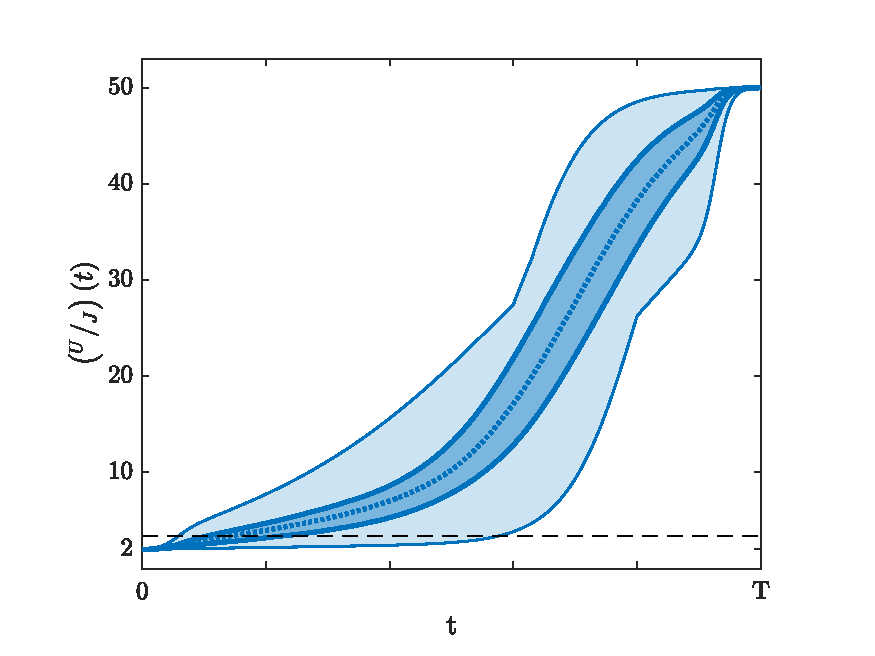
\includegraphics[width=0.7\textwidth]{Figures/LinSigSeed.pdf}
    \caption{\textit{Distribution of seeds used for optimization. All seeds lie within the lightly shaded region, while the darker region contains the 25-75 percentile of seeds. Lastly, the dotted line is the median value of the seed. The dashed line signifies the point of the Bose-Hubbard phase transition.}}
    \label{fig:LinSigSeed}
\end{figure}
Figure \ref{fig:LinSigSeed} shows the distribution of seeds used for the optimizations. Due to control parameter being the interaction strength of the Bose-Hubbard model, the phase transition occurs at quite a low control value. Hence, the initial part of the seed is a slowly increasing linear ramp, which crosses the point of the phase transition with a small slope. A shape function has been multiplied to the seeds enforcing a horizontal slope at the start and end of the duration, which helps avoiding any kinks in the control curve.



\section{Optimization of Dynamics in 5-Site Lattice} \label{sec:5partOptimization}
Previous studies of ramp sequences for the superfluid to Mott-insulator have employed the gradient-free Nelder-Mead optimization method \cite{Doria2011,FrankBloch}. Thus, to illustrate the power of interior point methods in non-linear and highly constrained problem, the same optimization problem was solved using both Nelder-Mead and interior point methods. While the framework is designed to conduct optimizations on larger systems, for the comparison of these two methods a 5-site lattice system with unit occupancy will suffice. Due to the small size of the system, no maximum bond dimension was required. Instead, a truncation threshold of $\epsilon_t = 10^{-8}$ was used. Furthermore, the relative tolerance used by the IPOPT library for determining convergence was set at $\varepsilon_t = 10^{-8}$. The optimization was carried out using a tolerance of $\varepsilon_t = 10^{-7}$ as well, however, the higher tolerance did not cause any notable change in neither obtained fidelity nor convergence rate, whereby these results are omitted.
Lastly, a regularization factor of $\gamma = 10^{-6}$ was employed. Since the control is parametrized using a linear combination of smooth functions, the effect of the regularization term is limited. Nevertheless, it does help the optimization algorithm avoid greatly varying controls during its initial iterations.
 

\subsection{Determining the Quantum Speed Limit}
In order to determine the quantum speed limit, one must solve the optimization problem for a series of durations, as calculating the quantum speed limit is otherwise a formidable task. In a complex quantum system, unit fidelity is only obtainable at very long duration. Therefore, one must decide on a fidelity threshold at which the obtained final state is sufficiently close to the target state. When deciding on this threshold, one must consider the size of the systems, as high fidelities are generally harder to obtain for larger systems. In \cite{MajaJulie} a similar optimization was made for lattice system of 3 sites. There, an infidelity threshold of $I_{\mathrm{QSL}} = 10^{-3}$ was used, which will be adopted for this optimization.
Since the result of the optimization often depends on the initial guess, 50 optimizations were carried out using both Nelder-Mead and interior point methods. The seeds were drawn for the distribution of ramps shown in figure \ref{fig:LinSigSeed}. For the following calculations a chopped basis size of $M = 20$ was chosen.

Figure \ref{fig:FidelityDuration} shows the final fidelities obtained for the superfluid to Mott-insulator transfer in the 5-site Bose-Hubbard system. While both methods manage to produce high fidelities, the interior method is clearly consistently better at every duration.
\begin{figure}[h!]
    \centering
    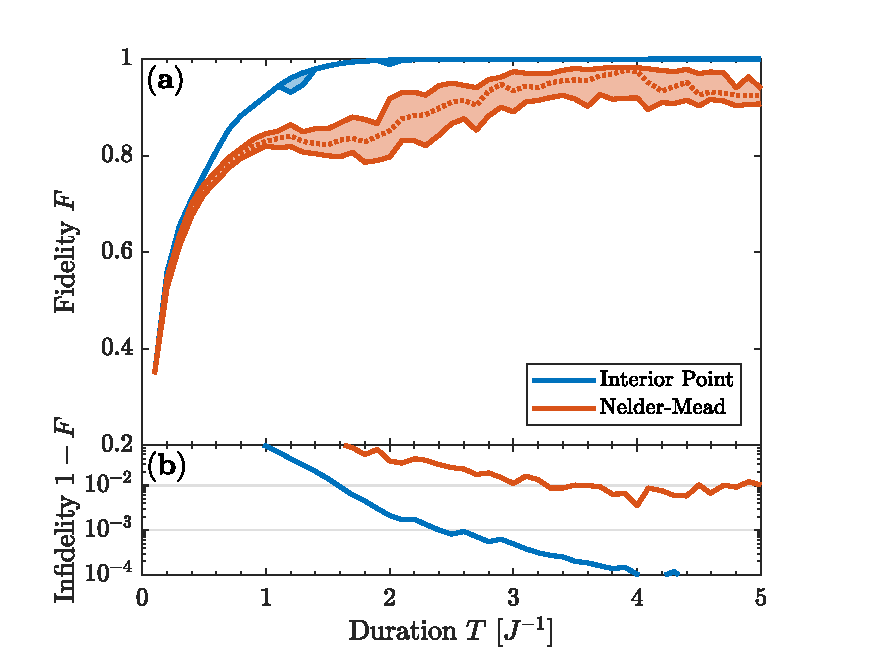
\includegraphics[width=0.9\textwidth]{Figures/L5/FidelityDuration.pdf}
    \caption{\textit{Final fidelity obtained for optimal control at various durations. \textbf{(a)} Median fidelity achieved marked by a dotted line, while the shaded area displays the $25\%$- and $75\%$-quartiles of the solutions. \textbf{(b)} The lowest infidelity achieved for each duration. }}
    \label{fig:FidelityDuration}
\end{figure}
In part \ref{fig:FidelityDuration}(a) the $25\%$- and $75\%$-quartiles along with the median of the solutions are displayed. At short durations the system can not evolve fast enough from the initial state to reach the target state, hence only low fidelities are obtained. The shortest duration of $T = 0.2 \; J^{-1}$ is almost a magnitude smaller than the time-scale of the tunneling. Therefore, the system can barely change from its initial configuration, whereby the different optimization methods produce identical results. However, as the system is given more time to evolve, the interior point method is much better at finding high-fidelity ramp sequences. Furthermore, the interior point method finds the optimal solution much more consistently, as the $25\%$- and $75\%$-quartiles of the solutions are almost indistinguishable from the median.

Information regarding the control landscape can be inferred from the variance in obtained fidelities. A small variance points towards a simple landscape with few local minima, while landscapes with many suboptimal solutions should produce a larger variance in obtained results. For short durations the system barely has time to change, whereby only very few solutions are possible. Therefore, the landscape is very simple, which is reflected in the extremely small variance produced by the interior point method. However, despite the simple landscape, the Nelder-Mead method converges to very different solutions. This is most likely due to the high convergence tolerance used for the Nelder-Mead optimizations, as only few improvements will be made for an already good starting guess. For comparison, a series of optimization were made using poor initial seeds for the Nelder-Mead method. Surprisingly, initiating the algorithm from an ill-behaving ramp actually caused it to converge towards the same solution as the interior point method. However, at longer durations, the optimizing using poor seeds led to considerably worse solutions as those displayed in figure \ref{fig:FidelityDuration}. Employing a lower tolerance should therefore result in better solutions achieved by the Nelder-Mead method, although this would significantly increase the number of function evaluations required for convergence. As shown in the next section, the Nelder-Mead method already has a very low convergence rate, whereby lowering its tolerance would severely lower its efficiency.

Figure \ref{fig:FidelityDuration}(b) displays the best solutions obtained for each duration. Plotting the result as an infidelity on a log scale clearly illustrates that the achieved fidelity continues to improve for longer durations. From the predetermined infidelity threshold, the quantum speed limit for the superfluid to Mott-insulator transition in a 5-site system can be inferred. Here, the interior point methods produces a quantum speed limit of $T_{\mathrm{QSL}}^{\mathrm{IP}} \sim 2.4 J^{-1}$ while it is $T_{\mathrm{QSL}}^{\mathrm{NM}} \sim 3.2 J^{-1}$ for the Nelder-Mead method. 
At long durations many optimal solutions exists, whereby the variance in results should be rather low. At durations on the order of $T \sim 5 J^{-1}$, the system has been evolved for timescales comparable to the tunneling time from one end of the lattice to the other. Thus, the duration is sufficient for the system to realize most of its possible configurations. Hence, both optimization algorithms should be capable of consistently finding high-fidelity solution, which is confirmed by the very low solution variance in figure \ref{fig:FidelityDuration}(a) for long durations. Meanwhile, for duration on the order of $T \sim 2 J^{-1}$  the evolution of the system is more restricted, whereby the impact of finding a good control sequence is larger. In fact, comparing the best solutions of figure \ref{fig:FidelityDuration}(b) reveals that the largest relative difference in obtained infidelity between the two methods occurs for these medium-long durations.\\

Previous optimizations of the superfluid to Mott-insulator phase have employed alternative figures of merit to the fidelity \cite{Doria2011,FrankBloch}. There, a rescaled variance of the particle number in each of the central sites of the lattice was employed. Although this figure of merit is less sensitive to system size than the fidelity, it does have some less favorable properties: First, multiple particle configurations different from unit occupancy of each site can achieve a vanishing particle number variance. Furthermore, the pure state of a single particle on each lattice site only becomes the ground state as the lattice depth tends towards infinity. Therefore, the number-variance figure of merit does not steer the state towards the ground state at the final control value, which will result in residual oscillations of the system after the control sequence. Therefore, the fidelity is a much better choice of figure of merit for the purpose of a state transfer to the ground state at a given control value.


\subsection{Convergence Rate}
Although obtaining a high fidelity is an impressive feat, most optimization algorithms should be capable of achieving high fidelities if a low enough convergence tolerance is employed. However, choosing a too high convergence tolerance will result in the algorithm running for long periods of time while only achieving minor improvements to the result. Therefore, it is important to investigate the convergence rate of the different methods, as their efficiency is extremely important for applications on larger systems.
\begin{figure}[h!]
    \centering
    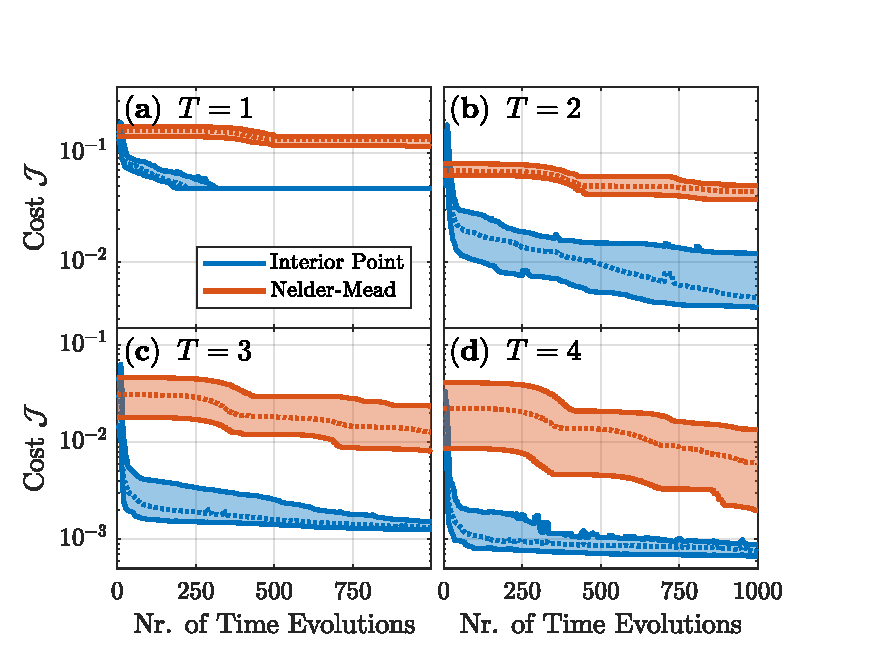
\includegraphics[width=0.9\textwidth]{Figures/L5/CostProgress.pdf}
    \caption{Optimization progress of the different optimization algorithms at various durations. The durations are in units of inverse tunneling strength. The dotted line marks the median cost \eqref{eq:grapeCost} at a given number of time evolution, while the shaded area illustrates the $25\%$- and $75\%$-quartiles of the current solutions.}
    \label{fig:CostProgress}
\end{figure}

The optimization process of the two algorithms tested is very different, as the Nelder-Mead method solely evaluates the cost function \eqref{eq:grapeCost}, while the interior point method requires both the gradient \eqref{eq:costGradient} to compute the step-direction and the cost function for a line search determining the step size. In both the computation of the cost and the gradient, the most resource-consuming calculations are the time evolutions of the state. Here, the computing the cost requires $N$ propagations of the initial state, while $2 N$ propagations are needed for evaluating the gradient. If the gradient and the cost are computed for the same control sequence, one only needs to propagate the initial state once thereby saving a full time evolution. For the interior point method, this will be the case for the first function evaluation in each iteration, however, each step of the line search will be done using a different control, whereby the initial state must be propagated anew.
Therefore, when comparing the convergence rate of the two methods, one should examine their obtained cost at a given number of time evaluations. Such a comparison is shown in figure \ref{fig:CostProgress} for a series of durations. Examining the progress of the two algorithms, one will notice that they behave quite differently. While starting at the same cost, the interior point method very quickly finds a control producing a much higher fidelity. This is possible through the gradient, which yields the optimal stepping direction for the optimization algorithm. Meanwhile, the Nelder-Mead method progresses by flipping its highest-lying vertex across the opposite edge \cite{wright}. As a result, the progress of the Nelder-Mead method is much more steady albeit slow.
An interesting feature of the interior point method is that the cost does not monotonically decrease, as the method sometimes settles for a worse cost. This is due to the algorithm solving a series of subproblems for different barrier heights. If the barrier height at some point is increased while the current optimization point lies close to the infeasible region, the cost will necessarily increase resulting in the small spikes visible in figure \ref{fig:CostProgress}.\\

The optimization progress is determined both by the individual algorithm but also by the underlying optimization landscape. For a short duration of $T=1 J^{-1}$, the optimization sequence is on the time scale of a single tunneling event. Therefore, only few possible configurations of particles are realizable, and the interior point method consistently finds the same solution using only very few time evolutions.

Curiously, the interior point method struggles the most at quickly finding an optimal solutions for the medium-long duration of $T = 2 J^{-1}$. As argued earlier, this regime is the most difficult to control, as the duration is sufficiently long to modify the configuration of particles in the lattice, while being too short for all configurations to be realizable. Therefore, the impact of having an optimized control will be the largest for medium-long durations. The large variations in the interior point cost points towards a complex optimization landscape, where the algorithm will take multiple different paths towards the optimum depending on the initial guess.

Finally, at long durations the optimization landscape becomes rather simple again, as many different control sequences will lead to a high fidelity. This is apparent from the almost flat bottom of the distribution of obtained solutions, which essentially marks a highest possible fidelity attainable at the given duration. At longer durations this fidelity becomes even higher, although not by much.\\

Clearly, the interior point method outperforms the Nelder-Mead algorithm both in terms of obtained fidelity and convergence rate. Therefore, investing additional resources into computing the gradient of the cost function definitely seems worth it.



\subsection{Optimized Ramp Sequences}
It is of interest observing how the system actually evolves when subjected to an optimized control sequence. As argued earlier, durations around $T \sim 2 J^{-1}$ are the hardest to optimize for the 5-site system. Therefore, the evolution expectation value of the number operator, $\braket{\hat{n}_i}$, was calculated for the highest fidelity control sequence achieved using the interior point method for $T = 2 J^{-1}$. Furthermore, the control was extended for an additional $T ' \approx 0.5 J^{-1}$ to illustrate the behavior of the system after the control sequence. The results are shown in figure \ref{fig:ExtendedRamp5}, which also displays the difference in fidelity between the initial guess and the optimized sequence.
\begin{figure}[h!]
    \centering
    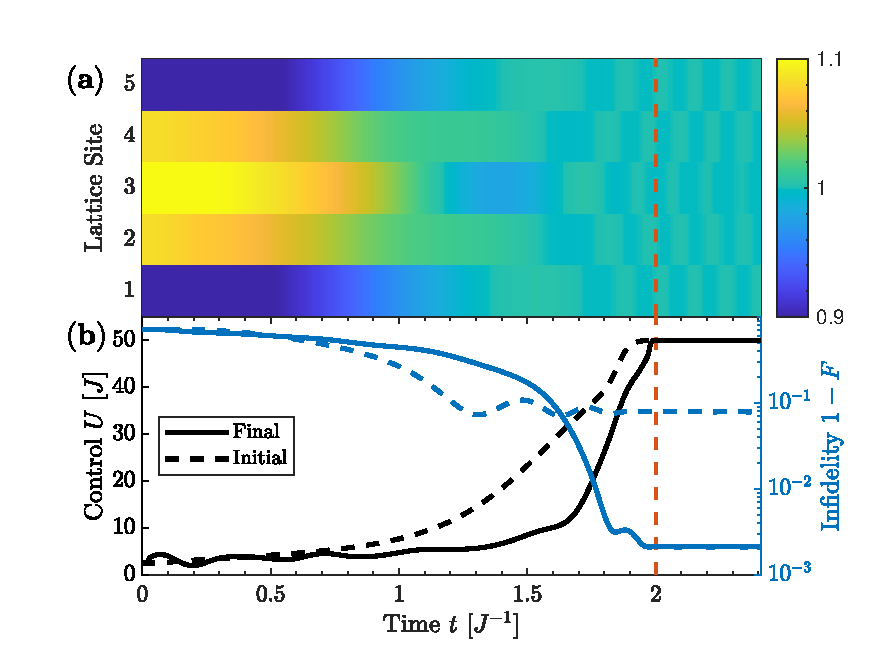
\includegraphics[width=0.9\textwidth]{Figures/L5/RampPlot.pdf}
    \caption{Solution with highest fidelity achieved for duration $T = 2 J^{-1}$ using the interior point method. The dashed, red line marks the end of the duration $T$, after which the system is further evolved according to the final control value. \textbf{(a)} Expectation value of the number operator, $\braket{\hat{n}_i}$, for each site of the lattice during optimal ramp sequence. The coloraxis has been rescaled to show small fluctuations. \textbf{(b)} Initial and optimized ramp sequences along with the corresponding evolution of fidelities.}
    \label{fig:ExtendedRamp}
\end{figure} 

In figure \ref{fig:ExtendedRamp5}(a) the expectation value of the number operator is plotted for each site during the ramp. Initially the system is in the superfluid phase, whereby the its energy is minimized by de-localizing the particles across the lattice. Due to the open boundary conditions, particles can only tunnel in one direction at the outer sites, which effectively causes a depletion of population. 
As the system is evolved towards the Mott-Insulating state, having multiple particles at the same sites becomes very energetically unfavorable. Hence, the target state has approximately only a single particle at each site, where any deviations are due to a finite value of $J/U$.
The optimized ramp brings the system very close to the target configuration of particles, which can be observed near the dashed red line marking the end of the duration, $T$. Some imperfections are present, although their magnitude is exaggerated by the logarithmic color axis.
After the duration of the optimized control sequence the system is further evolved according to $U(T)$. During this additional evolution, oscillations in the population are clearly visible. These oscillations can be attributed to two things: First, if the final state is not the ground state of $\hat{H}(U(T))$, then the system will not be in equilibrium. Therefore, the non-equilibrium dynamics will persist after the control duration. As the final infidelity is around $I(T) \sim 2 \cdot 10^{-3}$, the final state has small deviations from the ground state, whereby this explanation is the most likely. 
Secondly, the oscillations may be due to number fluctuations frozen in by the Kibble-Zurek mechanism. However, the Kibble-Zurek mechanism should be more prominent at longer time scales, when the critical point is crossed slowly. Nevertheless, it may partly be causing the visible oscillations in population.

Meanwhile, in figure \ref{fig:ExtendedRamp5}(b) the initial and optimized control is plotted together with their resulting infidelities. Optimizing the initial seed utilizing the interior point method has resulted in a reduction of almost two magnitudes in obtained infidelity.
While the initial ramp is fairly smooth, the optimized ramp wiggles a bit during the first three quarters of the duration followed by a sharp upswing towards the final control value. The steep increase in the control towards the end is very similar to the adiabatic-like ramp sequence proposed in \cite{Zakrzewski2009}. However, the initial oscillating behavior is highly non-adiabatic, as its oscillations appear to cross the critical point at $(U/J)_{\mathrm{crit}} = 3.37$ multiple times. It should be noted, that this value of the critical point was computed in the thermodynamic limit, whereby it is most likely slightly different for a finite sized system. However, crossing the critical point multiple times may cause interference of generated excitations, essentially creating a shortcut towards the target state. 
In fact, optimized ramp sequences for shorter durations had oscillations with even larger amplitude. Meanwhile, for long durations the solutions could reach a high fidelity through a more adiabatic-like ramp shape.


\subsection{Control Basis Size}
Unlike GRAPE, which takes the full optimization space into account, the chopped basis parameterization employed in GROUP results in a much smaller dimension of the optimization space. The chopped basis does not necessarily span the entire solution space, almost it may be sufficient for the representation of the optimal solution. However, if the chosen basis size is too small, artificial minima may be introduced to the control landscape due to the incompleteness of the basis \cite{Rach2015}. 
The chopped basis employed for both the interior point and Nelder-Mead calculation contain basis functions of the form $f_n = \sin \left( \omega_n t / T \right)$, where $\omega_n = n \pi$ are a set of increasing frequencies.
To investigate the basis size required to describe the optimal solutions, a series of optimizations were made for various basis sizes for the duration $T = 2 J^{-1}$. 
\begin{figure}[h!]
    \centering
    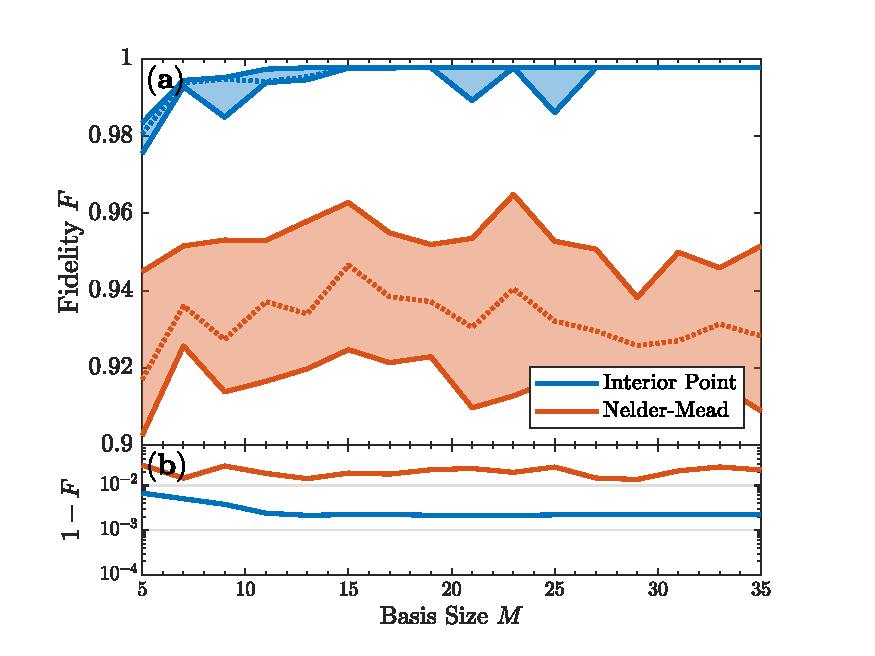
\includegraphics[width=0.9\textwidth]{Figures/L5/FidelityBasisSize.pdf}
    \caption{Final fidelity obtained for optimal control at various chopped basis sizes, $M$, for duration $T = 2 J^{-1}$. \textbf{(a)} The dotted line marks the median fidelity achieved, while the shaded area displays the $25\%$- and $75\%$-quartiles of the solutions. \textbf{(b)} The lowest infidelities achieved for each basis size.}
    \label{fig:FidelityBasisSize}
\end{figure}

The results of a scan over the chopped basis size, $M$, can be seen in figure \ref{fig:FidelityBasisSize}. The calculations were repeated 50 times for each basis size. Starting with the interior point method, the algorithm consistently finds good solutions for basis sizes larger than 15. Although their are a few exceptions, these lower fidelities are likely due to the algorithm getting stuck in local minima already present in the landscape. For $M < 15$ the variance in obtained fidelity clearly increases, which most likely is due to the introduction of artificial minima to the landscape. In figure \ref{fig:FidelityBasisSize}(b) the infidelity of the best solutions at each basis size is displayed. Here, the best solutions for the interior point method start to worsen around $M \sim 11$. The discrepancy in basis size between when the best solution and when the overall solutions become worse is causes by the fact that the optimal may still be realizable using only a few frequencies. Meanwhile, lowering the basis size will introduce an increasing number of artificial minima, until not even the optimal solution is spanned by the basis.
Meanwhile, the Nelder-Mead method produces very varying results, which can be attributed to the algorithm rather than the chopped basis size. While the solutions do appear to become worse for low values of $M$, the inconsistency of the algorithm makes it hard to draw a conclusion on the appropriate basis size. An investigation of a different control problem showed the final fidelity becoming worse for large basis sizes when employing the Nelder-Mead method, as the algorithm struggles optimizing too many parameters at once \cite{sorensen2018}. However, at the basis sizes investigated here, no such phenomenon is apparent.


\section{Application on Larger Systems} \label{sec:appLargeSystems}

The framework already contains all the components required for applications on larger systems, however, in larger the systems the effects of the open boundaries of the lattice is much smaller, whereby a much higher entanglement entropy is expected. Therefore, optimization of larger systems is infeasible employing the very low degree of truncation used for the smaller system. 

When applying the same settings to a system of 15 sites the optimization became increasingly slow for longer durations. Since no maximum bond dimension was specified, the matrices of the tensor network continued to grow in size, as entanglement built up in the system following the phase transition. As the cost of applying the tDMRG propagator scales quadratically with the bond dimension of the state, the time-evolution became increasingly slow. Furthermore, the GRAPE algorithm stores the state at each time step to efficiently compute the gradient, which causes the program to run out of available memory in certain cases. Thus, an analysis of the growth of entanglement within the system is necessary, if the framework is to be applied to larger systems.\\

Further improvements to the convergence rate may be achieved by calculating the Hessian of the cost function. For the purpose of this thesis, the Hessian was approximate using the L-BFGS algorithm, however, this approximation only becomes sufficiently accurate after multiple iterations. Since interior point methods solve a series of subproblems for decreasing barrier heights, the L-BFGS approximation must be restarted multiple times thus reducing its effectiveness \cite{Wachter2006}. On the other hand, supplying interior point methods with analytically derived gradient should result in superlinear convergence \cite{wright}.

A full derivation of the general GRAPE Hessian is presented in Appendix \ref{chap:Hessian} along with the altered version for the Suzuki-Trotter propagator. If both the forward propagated initial state and the backwards propagated target state is kept at each time step, the computation of the Hessian requires an additional $N(N - 1)/2$ step propagations, where $N$ is the total number of time steps of the ramp duration. However, these propagations can be separated into $N$ parallel calculations, which should significantly reduce the computational time of the Hessian. Note, that storing the backwards propagated target state would result in a doubling of the required memory occupied by the algorithm. Therefore, a suitable truncation of the tensor bond dimensions is required for the implementation of the Hessian.

In addition to increasing the convergence rate, valuable information regarding the optimization landscape can be extracted from the Hessian \cite{Shen2006}. Therefore, the addition of the Hessian to the framework may be a necessary step towards application on large systems, however, its implementation is outside the scope of this thesis.


\subsection{Spreading of Correlations and Entanglement}
Truncations of the matrix product state are necessary when optimizing control sequences for large systems, however, the truncation effectively creates a low-entanglement representation of the system. Hence, understanding the growth of entanglement within the system is crucial for the application on larger system. Furthermore, correlations within the system are essential to characterizing the system, whereby studying their evolution versus that of the entanglement entropy will provide valuable insight into the underlying dynamics of the system.

For this study a Bose-Hubbard system of 20 sites and particles was chosen. In a 20-site system, the overall effects of the open boundaries are much smaller, whereby the dynamics in this system are comparable to those of even larger lattices.
Previous studies have shown that the ramping speed greatly affects the dynamics of the system \cite{Lauchli2008,Braun2015}. Therefore, two very different ramps from $U(0) = 2.5 J$ to $U(T) = 50 J$ were examined: An abrupt quench to the final vale, and an exponential ramp typical from experimental procedures. Both ramps lasted a duration of $T = 3 J^{-1}$ and utilized Trotter steps of size $\Delta t = 5 \cdot 10^{-3} J^{-1}$. Furthermore, the maximum occupation at a single sites was limited to 7 bosons, which is relatively high and therefore should not affect the results \cite{Braun2015}. The analysis was carried out using a high truncation threshold of $\epsilon_t = 10^{-8}$ and a maximum bond dimension of $D = 1000$, whereby the entropy was barely limited.\\
\begin{figure}[h!]
    \centering
    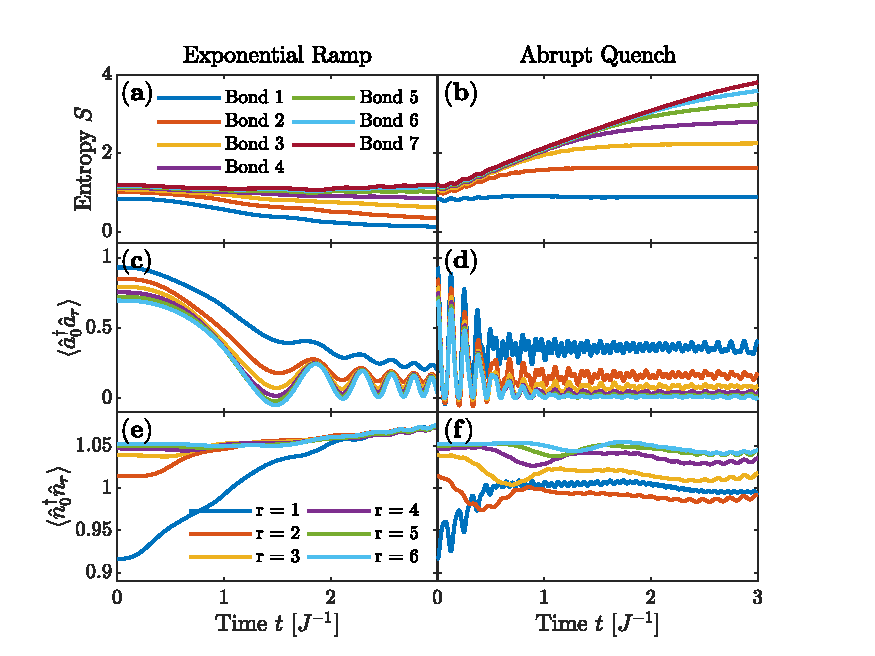
\includegraphics[width=\textwidth]{Figures/L20/EntanglementGrowth.pdf}
    \caption{Dynamical evolution of entanglement entropy and correlations during different types of ramps from $U(0) = 2.5 J$ to $U(T) = 50 J$. \textbf{(a-b)} von-Neumann entropy \eqref{eq:vNEntropy} for bipartitions of the lattice at various bonds, with bond 1 being between lattice sites 1 and 2 and so on. \textbf{(c-d)} Single-particle correlations for different distances $r$. \textbf{(e-f)} Rescaled density-density correlations for different distances $r$.}
    \label{fig:EntanglementGrowth}
\end{figure}

Figures \ref{fig:EntanglementGrowth}(a-b) display the von-Neumann entropy \eqref{eq:vNEntropy} for bipartitions of the lattice at different bonds.
In the case of the exponential ramp, the entanglement entropy between approximately equal sized blocks of the lattice remains almost constant throughout the entire duration. In fact, the entropy across the outer bonds decreases a relatively large amount. Near a critical point, the correlation length and entanglement should diverge for an equilibrium state \cite{Zurek2005}. However, since the system crosses the phase transition dynamically, the ground state decays into a linear combination of excited states, whereby the divergent behavior of the entropy is avoided. Since the exponential ramp is rather slow, it can be considered adiabatic for parts of the duration, whereby no excitations and entanglement is generated. For such a ramp, the dynamics will be influenced by the Kibble-Zurek mechanism \cite{Braun2015}.

On the contrary, the sudden quench in the interaction strength causes a rapid increase of entanglement. Quench dynamics are limited by the Lieb-Robinson bounds \eqref{eq:LiebRobinsonBound}, which is apparent from linear increase in entanglement with slope independent of the block size, $l$.  The saturation value of the entropy depends linearly on the block size, which effectively defines a maximum entropy propagation velocity $v_e$. A linear growth of entropy up to times $t = l/2 v_e$ has been shown for different models \cite{Lauchli2008,Eisert2006,Amico2008,Calabrese2005}, confirming that the spreading velocity is limited by a universal bound. A similar study the Bose-Hubbard model on a 32-site lattice \cite{Lauchli2008} yielded very similar results, whereby the dynamics appear relatively independent of system size.
Thus, the quantum state during a slow ramp can be accurately represented using only a small bond dimension. Meanwhile, a high bond dimension is required to fully describe the rapidly increasing entropy during a fast ramp sequence. \\

Next, the single-particle correlations, $\braket{\hat{a}_{0}^{\dag} \hat{a}_{r}}(t)$, during the two ramps were examined. For comparison it is worth looking at the equilibrium correlations and density matrices previously shown in figure \ref{fig:DensityMatrices}. In equilibrium one observes very long-ranged correlations in the superfluid phase, while the correlations decay exponentially for the Mott-insulation state. Figures \ref{fig:EntanglementGrowth}(c-d) display the single-particle correlations during the ramp sequence for various distances, $r$, from a reference site. Here, the 7th site of the lattice was chosen as reference to avoid the effects of the boundaries of the lattice.
Considering the exponential ramp first, the correlations decrease for the first half of the duration followed by a series of damped oscillations. Around the critical point, the Kibble-Zurek mechanism suggests a decay of correlation length following a power law \cite{Zurek2005}. While this is not entirely obvious from figure \ref{fig:EntanglementGrowth}(c), the correlation length clearly decreases during the first third of the duration, after which it starts growing again. The second half of the sweep duration features large oscillations in the correlations. The Kibble-Zurek mechanism is responsible for freezing in fluctuations, although the superfluid to Mott-transition should predominantly feature number fluctuation. A study of the phase transition via an exponential ramp showed that one would observe Gaussian damped revivals of the phase coherence \cite{Schutzhold2006}. The Gaussian decay should be independent of the distance $r$, which appears to be the case in figure \ref{fig:EntanglementGrowth}(c), as the fluctuations decay relatively similar.

Compared to the exponential ramp, the single-particle correlations behave much more violently, when the system is quenched. Initially, the correlations oscillate with a period of $T_{osc} \approx 2 \pi / U(T)$. These oscillations originate from the spectrum of the interaction part of the Bose-Hubbard Hamiltonian. Consider the case of negligible tunneling, whereby the evolution of the single-particle correlations is
\begin{equation}
	\braket{\hat{a}_{i}^{\dag} \hat{a}_{j}}(t) = \sum_{ \{ n \} , \{ n' \}} c_{n}^{*} c_{n'} \Braket{ \{ n \} | \hat{a}_{i}^{\dag} \hat{a}_{j} | \{ n' \}} \; \delta_{n_i , n_{i}' +1} \; \delta_{n_j , n_{j}' -1} \; e^{i U(T) (n_j ' - n_i ' - 1) t} \; ,
	\label{eq:CorrelationEvolution}
\end{equation}
where $\{ n \}$ is the set of Fock states with $n_i$ particles on the $i$'th site, and $c_n$ are coefficients of a general state \cite{Lauchli2008}. Only Fock state pairs corresponding to a particle begin annihilated at site $j$ and created at site $i$ will contribute to $\Braket{ \{ n \} | \hat{a}_{i}^{\dag} \hat{a}_{j} | \{ n' \}}$. As a result, the frequencies of the time evolution are given by $U(T) (n_j ' - n_i ' - 1)$. For a Mott-insulator with unit occupation all sites are populated equally, whereby the corresponding frequency is $-U(T)$ yielding an oscillation period $T_{osc} = 2 \pi / U(T)$. However, when starting in a superfluid state, the number fluctuations will result in frequencies containing higher multiplies of $U(f)$. Thus, the amplitude of higher-order frequencies is determined by the starting value $U(0)$.
In this case, the initial value is rather close to the critical point, whereby higher-order frequencies are not apparent until the first-order frequency has decayed sufficiently. At $t \approx 0.5 J^{-1}$ a beat-like structure in the oscillations is visible signifying contributions from higher-order frequencies. 
The single-particle correlation evolution \eqref{eq:CorrelationEvolution} assumes a vanishing tunneling. However, any finite tunneling will cause a spread in the frequencies, which ultimately leads to the decay of the oscillations in time \cite{Kollath2007}. Such decaying revivals have been observed experimentally in a Bose-Hubbard system \cite{Greiner2002collapse}.

After the relaxation of the oscillations, the system reaches a quasi-steady state with only minor fluctuations. These residual fluctuation in the correlations can be interpreted as number fluctuations of the superfluid being "frozen in" during the quench. As these number-fluctuations may be long-lived \cite{Schutzhold2006}, the residual oscillations remain for longer times. 

Clearly, neither the exponential ramp nor the quench produces an equilibrium Mott-insulator, as the final state has large, oscillating correlation functions. Nevertheless, while not being a Mott-insulator, the quenched system reaches a quasi-steady state. An investigation of the problem in \cite{Kollath2007} revealed that the steady-state correlation lengths were determined mainly by the difference between the initial and quenched value of $U$. Thus, the final state could be categorized as belonging to one of two non-equilibrium phases: A \textit{non-thermal steady state} produced by a large quench, and a \textit{thermalized state} for smaller quenches. The state obtained here is distinctly non-thermal, as it retains a strong memory of its initial state.\\

Finally, the evolution of density-density correlations, $\braket{\hat{n}_{0}^{\dag} \hat{n}_{r}}(t)$, was investigated, as shown in figures \ref{fig:EntanglementGrowth}(e-f). Since the number operator, $\hat{n}_i$, commute with the interaction term of the Bose-Hubbard Hamiltonian, no large oscillations should be present in the strong coupling limit. For the case of the exponential ramp this is indeed the case, as the correlations at all distances decay towards the same constant value associated with equal population across the lattice. For a perfect Mott-insulator and unit occupancy the density-density correlations should converge to 1. However, as established earlier, the exponential ramp clearly does not produce the ground state Mott-insulator, whereby the deviations are expected. Interestingly, small oscillations in the correlations are present at later times for all distances. This is most likely caused by the superfluid number-fluctuations frozen in by the Kibble-Zurek mechanism.

When quenching the system, the density-density correlations behave much differently. Due to rapid change of the interactions, the correlations can no longer relax into a common value but are instead almost frozen in from the start. At short distances, the correlations appear increasingly Mott-like, while at longer ranges the large variances in population becomes apparent. Further examining the first half of the quench duration, it is clear that some signal is propagating through the system at what appears to be a constant velocity.
\begin{figure}[h!]
    \centering
    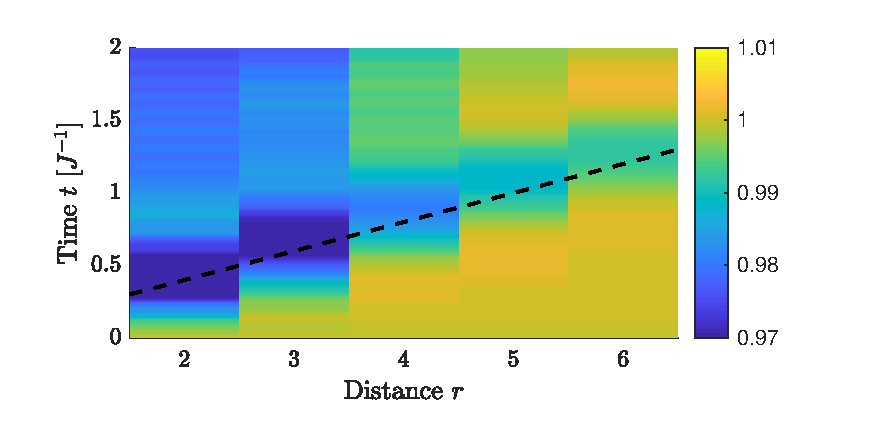
\includegraphics[width=0.8\textwidth]{Figures/L20/CorrelationLightCone.pdf}
    \caption{Time evolution of normalized density-density correlations $\braket{\hat{n}_{0}^{\dag} \hat{n}_{r}}(t) / \braket{\hat{n}_{0}^{\dag} \hat{n}_{r}}(0)$ after an abrupt quench. The correlations are spreading with a constant velocity, and the front of the evolution is marked by a dashed line.}
    \label{fig:CorrelationLightCone}
\end{figure}
Plotting the evolution of the density-density correlations as a function of distance produces figure \ref{fig:CorrelationLightCone}, where the light-cone-like propagation of correlations is very obvious. For distances $r >  v_c t$, with $v_c$ being the propagation velocity of correlation, the correlations are constant, despite the system having already undergone the quench. In the limit of very fast ramps (where a quench is instantaneous), the propagation of correlations can be interpreted as ballistically spreading quasi-particles \cite{Cheneau2012,Calabrese2006}. The propagation velocity of the correlations is bounded by the Lieb-Robinson bound \ref{eq:LiebRobinsonBound}, resulting in the effective light-cone. An even clearer light-cone was shown in \cite{Lauchli2008} by rescaling the correlations accordingly.\\

The exponential ramp and the quench represent two limits of ramping speeds. The exponential ramp is slow, whereby the system can react almost adiabatically, as no violent oscillations in the correlations are present. Nevertheless, the product of exponential ramp is clearly not a perfect Mott-insulator, as correlation functions point towards number fluctuations in the final state. However, since the entanglement entropy of the system does not increase during the ramp, the matrix product description of the state is very accurate at even long timescales.
On the other hand, the dynamics of the correlations following a quench are much more violent, as the ramp is essentially instantaneous. At long timescales, the system starts to reach a steady-state, although this state appears non-thermal from its correlations, whereby it has very different characteristics than the Mott. An optimal ramp will most likely contain elements from both fast and slow ramps in order to produce a high-fidelity Mott-insulator at a low ramp duration. 



\subsection{Required Bond Dimension for Non-Equilibrium Dynamics}
The main limiting factor when performing quantum optimal control is the computational cost of the time-evolution. Thus, for large systems it is vital to maintain a minimal bond dimension during the entire ramp duration. The previous analysis illustrated the dynamics of a 20 site system with unit occupation during a fast and a slow ramp. Here, the effect of truncating the tensors at various maximum bond dimension is investigated. As an exponential ramp causes no increase in the entanglement entropy of the system, the system should be much easier to simulate. Therefore, it is of interest just how few contributing eigenstates need to kept in order to produce a final state comparable to a non-truncated one.
For this analysis, an even slower, $T = 5 J^{-1}$, exponential ramp was used. The truncation threshold was kept at $\epsilon_t = 10^{-8}$, while the maximum bond dimension was varied. The calculation was carried out for Trotter step-sizes of $\Delta t = 5 \cdot 10^{-3} J^{-1}$ and $\Delta t = 10^{-2} J^{-1}$ and produced similar results. Here the results for a step size of $\Delta t = 10^{-2} J^{-1}$ are shown, as this step size is more likely to be used for the optimization of a larger system.\\ 

\begin{figure}[h!]
    \centering
    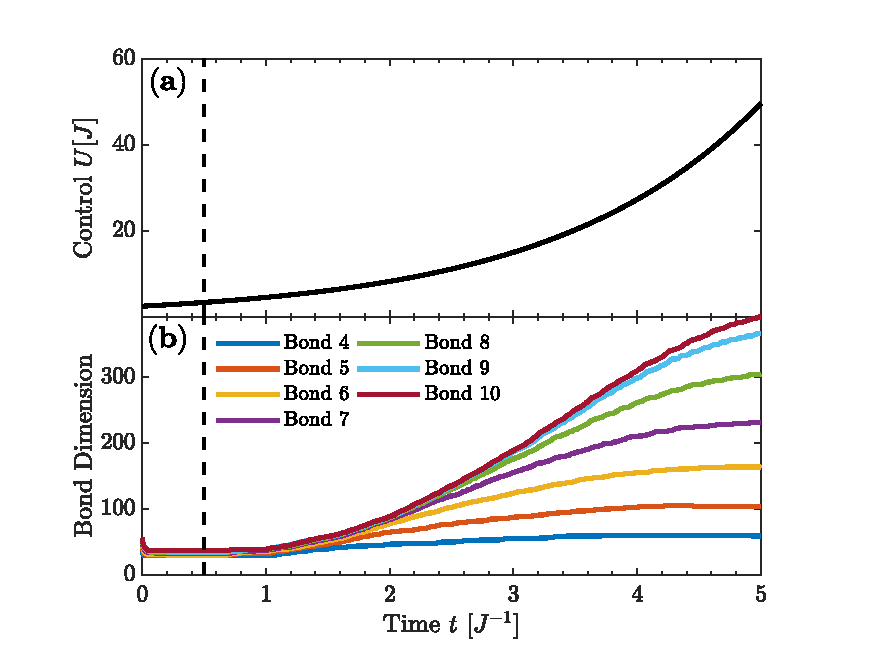
\includegraphics[width=0.9\textwidth]{Figures/L20/BondDimEvolution.pdf}
    \caption{ Evolution of bond dimensions during an exponential ramp. \textbf{(a)} The exponential ramp from $U(0) = 2.5 J$ to $U(T) = 50 J$. The crossing of the critical point is marked by the dashed line. \textbf{(b)} Dimension of various bonds of the matrix product representation of the quantum state. }
    \label{fig:BondDimEvolution}
\end{figure}
First, the growth of bond dimension during the ramp was investigated, which is shown in figure \ref{fig:BondDimEvolution}. In subfigure (a) the exponential ramp is shown, and the time at which it crosses the critical point is marked by a dashed line. The bond dimensions of the initial superfluid state evolved according to the ramp is displayed in figure \ref{fig:BondDimEvolution}(b). Initially, the bond dimension remains constant, which is expected from the previous results showing the entanglement entropy decreasing during the ramp duration. However, a short while after having crossed the critical point, the dimension of all inner bonds starts increasingly rapidly. This increase in bond dimension is very similar to the increase in entropy following a sudden quench, however, it is most unexpected in the case of the exponential ramp. Although the bond dimension of a matrix product state is expected to increase as it is time evolved \cite{Daley2004}, the truncation threshold of $\epsilon_t = 10^{-8}$ should maintain a low bond dimension throughout the duration.
\begin{figure}[h!]
    \centering
    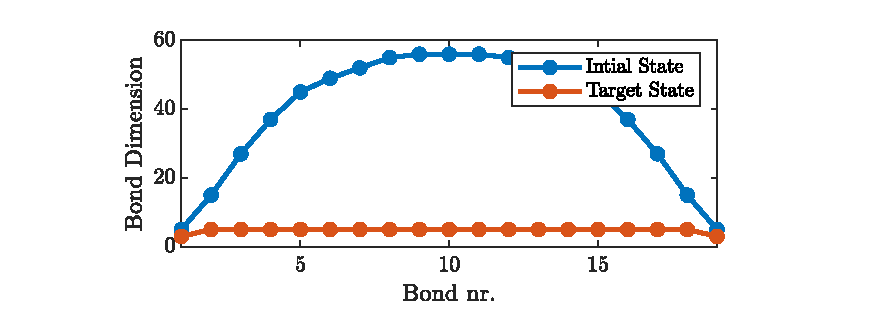
\includegraphics[width=0.9\textwidth]{Figures/L20/InitialBondDim.pdf}
    \caption{ Bond dimensions of the initial superfluid ground state for $U = 2.5 J $ and the target Mott-insulating ground state for $U = 50 J $.}
    \label{fig:InitialBondDim}
\end{figure}
For comparison, the bond dimensions of the initial and target states are illustrated in figure \ref{fig:InitialBondDim}. The superfluid ground state has long-ranged correlations resulting in a parabola-like distribution of bond dimensions. Meanwhile, the exponentially decaying correlations of the ground state Mott-insulator causes a flat distribution of bond dimensions, and the state is well represented using only very few eigenstates. Thus, the matrix product representation of the evolved state is very different from the ground state. However, when examining the entanglement and correlations following the exponential ramp in figure \ref{eq:CorrelationEvolution}, the high bond dimension seem redundant for the description of the state. Therefore, dynamically truncating the matrices at a low maximum bond dimension, $D$, should not alter the dynamics of the system considerably.

\begin{figure}[h!]
    \centering
    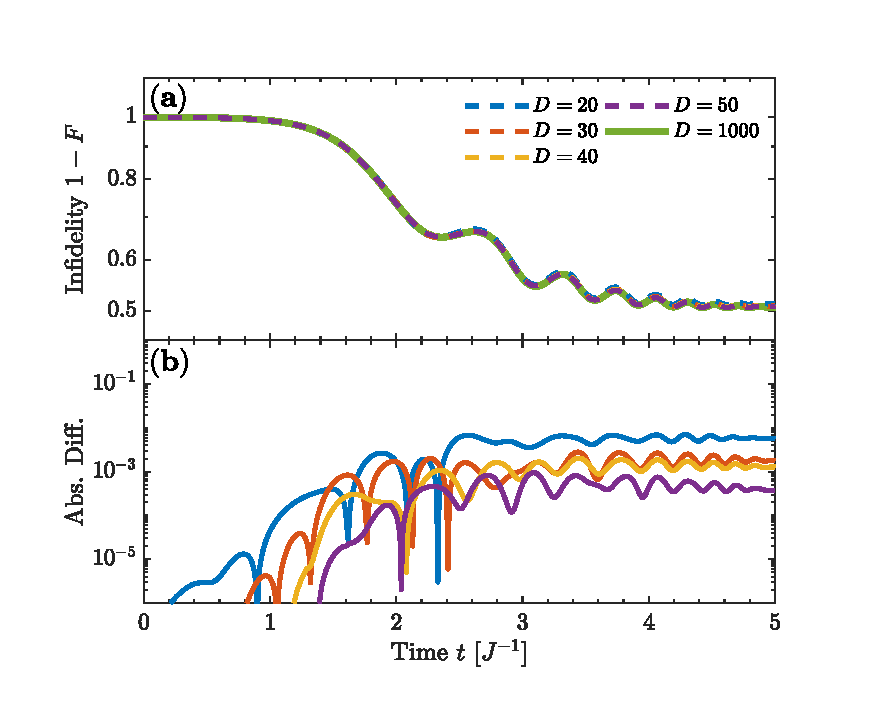
\includegraphics[width=0.9\textwidth]{Figures/L20/FidelityTruncation.pdf}
    \caption{ \textbf{(a)} Obtained infidelity with regards to the Mott-insulating ground state for the exponential ramp. The calculation was carried out for different maximum bond dimension $D$. \textbf{(b)} Absolute difference between infidelities obtained with no truncation ($D = 1000$) and those employing a maximum bond dimension.  }
    \label{fig:FidelityTruncation}
\end{figure}
To prove that the bond dimension of the evolved state is artificially high, the same initial state was evolved according to the same exponential ramp while begin truncated at a given maximal bond dimension, $D$. The results shown in figure \ref{fig:FidelityTruncation} reveal that the obtained infidelity barely changes when decimating the bond dimension. While a weak scaling with maximum bond dimension was expected \cite{Daley2004}, the amount of redundant information in the $D = 1000$ evolution is still surprising. According to figure \ref{fig:FidelityTruncation}(b), choosing a maximal bond dimension of $D = 30$ should produce a difference in infidelity a magnitude smaller than the threshold for the quantum speed limit. Meanwhile, the time evolution of the truncated state should proceed much faster, as the application of the propagator scaled quadratically with the bond dimension.

\begin{figure}[h!]
    \centering
    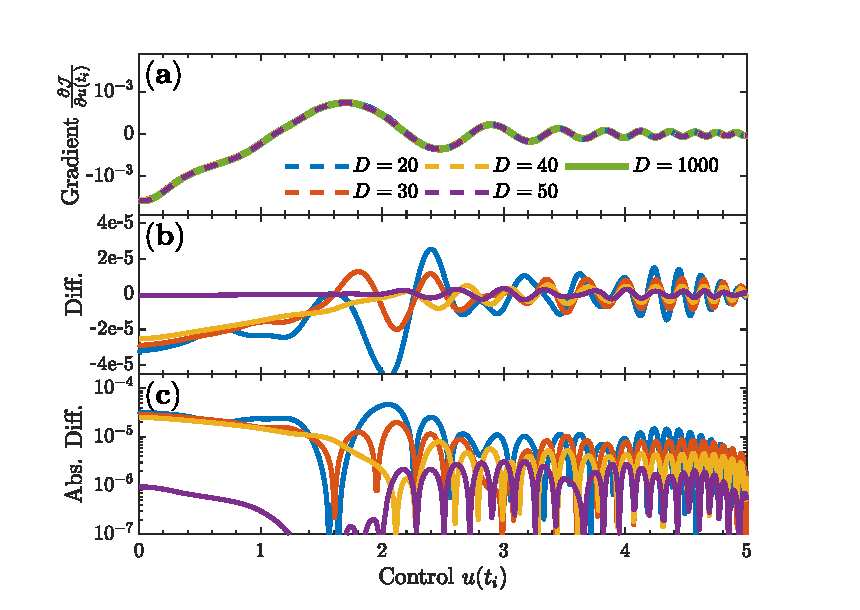
\includegraphics[width=0.9\textwidth]{Figures/L20/GradientTruncation.pdf}
    \caption{ \textbf{(a)} Gradient elements of the cost function \ref{eq:STcostgrad} for the exponential ramp. The calculation was carried out for different maximum bond dimension $D$. \textbf{(b)} Difference in gradient element between the non-truncated state ($D = 1000$) and the states having a maximum bond dimension. \textbf{(c)} Absolute value of the differences. }
    \label{fig:GradientTruncation}
\end{figure}
Lastly, it is also worth examining how the truncation affects the gradient elements, as having accurate derivatives is essential for a fast convergence rate \cite{deFouquieres2011}. Figure \ref{fig:GradientTruncation} shows the results of calculating the gradient elements \ref{eq:STcostgrad} for the exponential ramp without any regularization. Compared with the infidelity, the gradient scales more strongly with the maximum bond dimension. Therefore, the truncation is limited by the derivative of the cost function rather than the function itself. Unlike the infidelity, the gradient becomes gradually better during the ramp sequence. The same phenomenon is discussed in section \ref{sec:TrotterGrad} and is caused by the accumulated error when calculating $\ket{\chi (0)}$. 
While the bond dimensions of the matrix product state start growing rapidly after crossing the critical point, neither the infidelity nor the gradient show no signs of being influenced by the phase transition whatsoever. This discrepancy remains open for interpretation, however, it points towards optical control methods being well suited for studying phase transitions. 
\chapter{Conclusion}

This is a conclusion ....


%----------------------------------------------------------------------------------------
%	BIBLIOGRAPHY
%----------------------------------------------------------------------------------------

\printbibliography[heading=bibintoc]

%----------------------------------------------------------------------------------------
%	THESIS CONTENT - APPENDICES
%----------------------------------------------------------------------------------------

\appendix % Cue to tell LaTeX that the following "chapters" are Appendices

\chapter{Diagrammatic Representation of Matrix Product States} \label{chap:diagrams}

Due to the many indices, equations describing contractions of matrix product states are often quite hard to read. Therefore, the equations are often represented graphically through diagrams. Many variations of diagrams exists, however, they all follow some general rules:
\begin{itemize}
\item
Tensors are represented by nodes.
\item
Indices are represented by lines. Horisontal lines are \textit{bond indices}, while vertical lines are \textit{physical indices}.
\item
Tensors connected by a line are contracted over said bond.
\end{itemize}
Through these basic rules, most equations involving matrix product states can be expressed through diagrams. In this instance, the color or shape of a node provides information regarding the properties of the tensor. Therefore, the tensors shown in this thesis follow these guidelines:
\begin{itemize}
\item
Tensors part of an MPS are square-like. The color of the tensor denotes its normalisation, as shown in figure \ref{fig:MPStensors}. These different types of normalisation are part of of MPS canonical forms (see Section \ref{sec:canonical}).
\item
Tensors part of MPO's are grey and circular/elliptical depending on the number of sites they span over. These tensors have two vertical legs compared two the one leg of the MPS tensors.
\item
Matrices (tensors without any physical index) are depicted as a diamond. These often occur after a singular value decomposition. 
\end{itemize} 


\begin{figure}[h!]
\centering % <-- add this
\begin{subfigure}[t]{0.2\textwidth}
	\caption{}  	
  	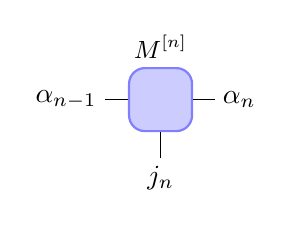
\begin{tikzpicture}[inner sep=1mm]
	\node[tensor, label={\small $M^{[n]}$}] (tensor1) at (0, 0) {};
	\node (index1) at (0, -1) {$j_n$};
	\node (index2) at (1, 0) {$\alpha_{n}$};
	\node (index3) at (-1.2, 0) {$\alpha_{n-1}$};
	
	\draw[-] (tensor1) -- (index1);
	\draw[-] (tensor1) -- (index2);
	\draw[-] (tensor1) -- (index3);
\end{tikzpicture}
\end{subfigure}
\hspace{5mm}
\begin{subfigure}[t]{0.2\textwidth}    
	\caption{}  	
  	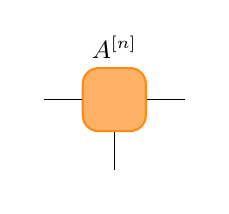
\begin{tikzpicture}[inner sep=1mm]
	\node[tensorl, label={\small $A^{[n]}$}] (tensor1) at (0, 0) {};
	\node (index1) at (0, -1) {};
	\node (index2) at (1, 0) {};
	\node (index3) at (-1, 0) {};
	
	\draw[-] (tensor1) -- (index1);
	\draw[-] (tensor1) -- (index2);
	\draw[-] (tensor1) -- (index3);
\end{tikzpicture}
\end{subfigure}
\hspace{5mm}
\begin{subfigure}[t]{0.2\textwidth}    
	\caption{}  	
  	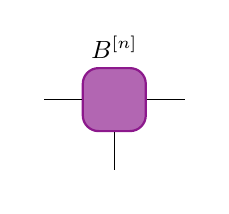
\begin{tikzpicture}[inner sep=1mm]
	\node[tensorr, label={\small $B^{[n]}$}] (tensor1) at (0, 0) {};
	\node (index1) at (0, -1) {};
	\node (index2) at (1, 0) {};
	\node (index3) at (-1, 0) {};
	
	\draw[-] (tensor1) -- (index1);
	\draw[-] (tensor1) -- (index2);
	\draw[-] (tensor1) -- (index3);
\end{tikzpicture}
\end{subfigure}
\hspace{5mm}
\begin{subfigure}[t]{0.2\textwidth}    
	\caption{}  	
  	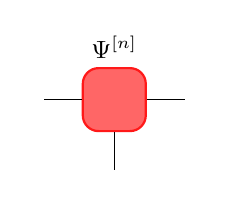
\begin{tikzpicture}[inner sep=1mm]
	\node[tensorc, label={\small $\Psi^{[n]}$}] (tensor1) at (0, 0) {};
	\node (index1) at (0, -1) {};
	\node (index2) at (1, 0) {};
	\node (index3) at (-1, 0) {};
	
	\draw[-] (tensor1) -- (index1);
	\draw[-] (tensor1) -- (index2);
	\draw[-] (tensor1) -- (index3);
\end{tikzpicture}
\end{subfigure}
\caption{\textit{The four different types of MPS tensors used in diagrams. \textbf{(a)} General tensor of un-specified normalisation. The indices corresponding to the tensor are labeled. The remaining tensors are: Left-normalised \textbf{(b)}, right-normalised \textbf{(c)}, central cite \textbf{(d)}. }}
\label{fig:MPStensors}
\end{figure}
	

\chapter{Example: Building an MPO from a Hamiltonian}
\label{chap:buildMPO}
Consider the Bose-Hubbard Hamiltonian , which consists of both nearest-neighbour tunneling terms and on-site interactions terms
\begin{equation}
	\hat{H} = - J \sum_{\langle i,j \rangle} \hat{a}_{i}^{\dag} \hat{a}_{j} + \frac{U}{2} \sum_{i} \hat{n}_i \left( \hat{n}_i -1 \right) \; .
	\label{eq:BHhamil}
\end{equation}
The Hamiltonian can be expressed as a sum of strings of operators - most of these being identities just like in equation \ref{eq:localOperator}. Moving through such a string from the right, one will at some point encounter one of 3 non-trivial operators. This can be summarized as 4 different possible states of the string of operators on a given bond:
\begin{enumerate}
	\item
	Only identities to the right of the bond.
	\item
	An $\hat{a}^{\dag}$ operator just to the right of the bond.
	\item
	An $\hat{a}$ operator just to the right of the bond.
	\item
	A completed tunneling \textit{or} the interaction term, $\frac{U}{2} \hat{n} \left( \hat{n} -1 \right)$, somewhere to the right.
\end{enumerate}
When moving through the string of operators from the right, only certain transitions between these state are possible. For instance $\boldsymbol{1 \rightarrow 1}$, where one starts in state 1, and the next operator is an identity. Likewise, $\boldsymbol{1 \rightarrow 2,3,4}$ are all possible, since these transitions represent the next operator being non-trivial. Next, $\boldsymbol{2 \rightarrow 4}$ completes the hopping $-J \hat{a}^{\dag} \hat{a}$ - a similar transition exists for the other hopping term $\boldsymbol{3 \rightarrow 4}$. Finally, the transition $\boldsymbol{4 \rightarrow 4}$ is needed to continue iterating through the operator chain after having passed the non-trivial operators. This can be encoded in the operator-valued matrix
\begin{equation}
 W^{[i]} \: = \: \begin{pmatrix}
\hat{I} & 0 & 0 & 0  \\
\hat{a}^{\dag} & 0 & 0 & 0  \\
\hat{a} & 0 & 0 & 0 \\
\frac{U}{2} \hat{n} \left( \hat{n} -1 \right) & -J \hat{a} & -J \hat{a}^{\dag} &  \hat{I}
\end{pmatrix} \; ,
\label{eq:MPOmatrix}
\end{equation}
which contains all the allowed transitions between the five state \cite{schollwock}. When one starts moving through the operator chain from the right side, one obviously begins in state 1 and ends in state 4. This can be encoded in the two vectors
\begin{equation*}
 \vec{v}_{left} = (0 , 0 , 0  , 1) \quad , \quad \vec{v}_{right} = (1  , 0 ,0 , 0)^T \; .
\end{equation*}
Thus, the Bose-Hubbard Hamiltonian can be written as an MPO 
\begin{equation}
	\hat{H} = \sum_{\boldsymbol{j}, \boldsymbol{j'}} \vec{v}_{left} \; W^{[1] j_1 , j_1 '} W^{[2] j_2 , j_2 '} \ldots W^{[N] j_N , j_N '} \; \vec{v}_{right} \; \ket{\boldsymbol{j}} \bra{\boldsymbol{j'}} \; .
	\label{eq:MPOhamiltonian}
\end{equation}
Often, the two closing vectors are implicitly multiplied unto the outer matrices for a cleaner notation. Observe how all of this was done without having to do a single numerical computation. The resulting MPO can now readily be applied to an MPS.
\chapter{Calculation of Condensate Fraction using DMRG Algorithm} \label{chap:CondFrac}
To illustrate the power of the DMRG algorithm, the following numerical analysis was conducted. As the system of interest is the Bose-Hubbard model described in eq. \eqref{BHhamil}, a suitable benchmark for the algorithm is attempting to calculate the critical point of the phase transition between the superfluid and Mott-insulator. The critical point was determined using the DMRG algorithm in \cite{Kuhner2000} by studying the correlations of the system. Here, an alternative approach is presented, which examines the condensate fraction.

According to the Penrose-Onsager criterion, a system is in the superfluid phase if and only if the largest eigenvalue, $\lambda_1$, of the single-particle density matrix, $\rho^{(1)}$, is macroscopic
\begin{equation}
	f_c = \frac{\lambda_1}{N_p} > 0 \; ,
	\label{eq:condensateFraction}
\end{equation} 
where $f_c$ is the condensate fraction, and $N_p$ is the total number of particles \cite{PenroseOnsager}. The condensate fraction can be used to determine which phase dominates the system, as
\begin{align}
	\lim_{N_p \to \infty} f_{c}^{\mathrm{SF}} &\to 1 \label{eq:SF_lim} \\
	\lim_{N_p \to \infty} f_{c}^{\mathrm{MI}} &\to 0 \; , \label{eq:MI_lim}
\end{align}
when the filling-fraction, $n = N_p/L$, is held constant.

To calculate the condensate fraction, the ground state of the system was found using a version of the DMRG algorithm implemented in the ITensor library \cite{ITensor}. Using the computed ground state, $\ket{\psi}$, the entries of the density matrix were calculated
\begin{equation}
	\rho_{i,j}^{(1)} = \bra{\psi} \hat{a}_{i}^{\dag} \hat{a}_{j} \ket{\psi} \; .
\end{equation}
Lastly, the condensate fraction was determined through eq. \eqref{eq:condensateFraction}.
The calculation was performed with varying $U/J$ for various system sizes of unit occupancy. The DMRG algorithm was set to perform 5 sweeps with a maximum bond dimension of 200.
In order to gauge the accuracy of the algorithm, the results for system sizes 4-10 were compared to a similar calculation using exact diagonalisation.
\begin{figure}[h!]
    \centering
    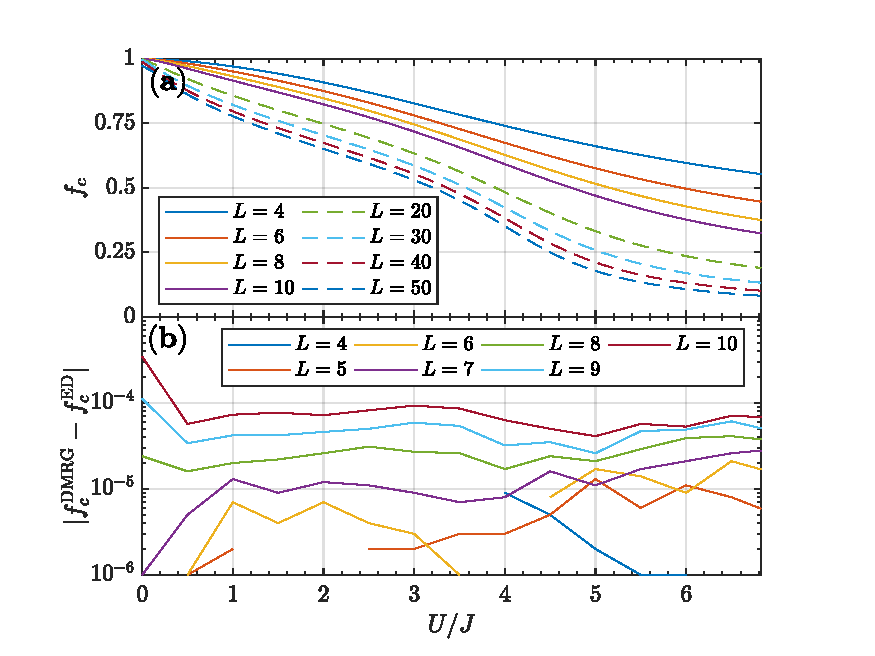
\includegraphics[width=0.7\textwidth]{Figures/CondensateFractionCompare.pdf}
 \caption{\textit{Condensate fraction calculated using the DMRG algorithm with 20 sweeps. The condensate fractions of the smaller systems ($L = 4 \ldots 10$) are compared with result obtained through exact diagonalisation.}}
 \label{fig:CondensateFraction}
\end{figure}
The upper part of figure \ref{fig:CondensateFraction} shows the condensate fraction for various $U/J$ calculated using the DMRG algorithm. In the limit $U/J = 0$, the condensate fraction is unit for the smaller systems, confirming the system is indeed in the superfluid phase. The condensate fraction never reaches zero as $U/J$ increases, since this is only achieved in the thermodynamic limit. However, the condensate fraction does decrease with increasing particle number, as would be expected. The lower half of figure \ref{fig:CondensateFraction}  displays the results of the DMRG calculation compared with exact diagonalisation. For small systems the two approaches obtain very similar results.

Attempting to use exact diagonalisation for large systems is futile, due to the exponential scaling of the Hilbert space \cite{Vidal2003}. However, this is not an issue using matrix product states, as the formalism only considers a tiny corner of the Hilbert space by following an area law. 
The dashed lines of figure \ref{fig:CondensateFraction} shows the results of the DMRG calculations for up to 50 particles. The condensate fraction behaves as expected in the $U/J \gg 1$ limit, as it tends towards zero for larger particle numbers. Note, in the superfluid limit the condensate fraction does not quite reach 1. For large systems the superfluid phase is gapless, whereby the ground state no longer follows an area law. For the system sizes investigated here, a small interaction will cause the spectrum to become gapped, however, in the $U/J = 0$ limit for large systems, the area laws will break down. Hence, the DMRG algorithm has to search a much larger part of the Hilbert space, which causes a worse approximation of the ground state. A possible solution to this issue is using more sweeps in the ground state search. Figure \ref{fig:sweepdependence} displays the condensate fraction in the Superfluid limit as a function of number of sweeps. Allowing the DMRG algorithm to perform additional search-sweeps clearly causes an improvement in the ground state description. 
\begin{figure}[h!]
    \centering
    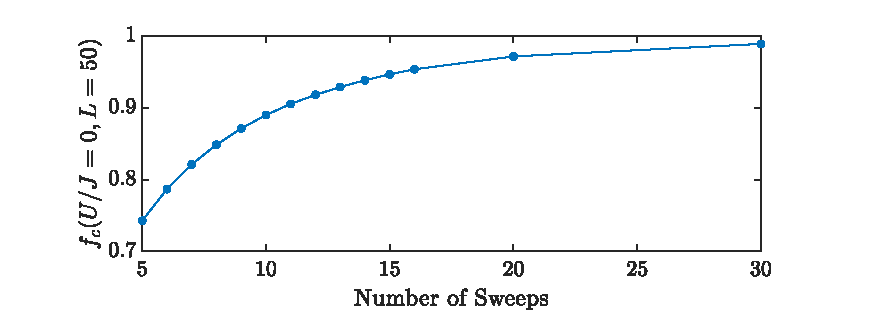
\includegraphics[width=0.7\textwidth]{Figures/CFsweeps.pdf}
    \caption{\textit{Condensate fraction as a function of number of sweeps of the DMRG algorithm in the superfluid limit. A max bond dimension of $D = 250$ was used.}}
    \label{fig:sweepdependence}
\end{figure}
Furthermore, increasing the maximal bond dimension, $D$, results in a more accurate long-range representation of correlations. Thus, calculating correlation functions for various values of $D$ is a great way of estimating the convergence of the correlations for a given length scale \cite{schollwock}.\\

In \cite{Kuhner2000} the critical point of phase transition between the Superfluid and Mott-insulator was determined as $\left( {U}/{J} \right)_{crit} = 3.37$. The result is achieved through examining the correlations of the systems. While correlations in Mott-insulators decay exponentially, superfluid correlations decay according to a power-law. The interface between the two phases has correlations following a power law determined by the Luttinger liquid parameter. The critical point, which is located at the tip of the Mott-lobes, was computed by determining the point at which the Luttinger liquid parameter was $K =  \frac{1}{2}$ \cite{Kuhner2000}.\\
Examining figure \ref{fig:CondensateFraction}, one notices a hump on the graph in the vicinity of the critical ratio, but no clear indication of a phase transition is present. In the thermodynamic limit one would expect the condensate fraction to drop to zero as the critical point is reached (as observed in 2D by \cite{Spielman2008}). However, at 50 particles the condensate fraction is only around $ f_c = 0.5$. One could extrapolate data from computations using different particle numbers in order to determine the location of the critical point. However, this would require computations using larger systems in order to minimize the boundary effects.
\chapter{Example: Quantum Speed Limit in Landau-Zener Model} \label{chap:LZexample}
To illustrate concepts from quantum optimal control theory, a state transfer within the Landau-Zener model is optimized using the GRAPE algorithm.\\
The Landau-Zener model is a two-level system with the general Hamiltonian
\begin{align}
	\hat{H}_{\mathrm{LZ}} = \begin{pmatrix}
    	 \Delta (t) & \Omega_R    \\
         \Omega_R & -\Delta (t) 		
    \end{pmatrix}  = \Omega_R \hat{\sigma}_x + \Delta (t) \hat{\sigma}_z \; , \label{eq:LZhamiltonian}
\end{align}
where $\Omega_R$ is the positive Rabi-frequency, $\Delta (t)$ is the detuning, and $\hat{\sigma}_i$ are the Pauli spin matrices. In such a system the detuning will be the control parameter, as it is easily to manipulate in an experimental setup. An advantage of the Landau-Zener system is that an analytical solution to the control problem exists for arbitrary initial and final states. Furthermore, two level systems can be illustrated on the Bloch sphere, which depicts the population of the two levels along with the relative phases. Consider the transfer between the initial state
\begin{equation}
\lvert \psi_0 \rangle = \cos{\left(\frac{\theta_0}{2}\right)} \lvert 0 \rangle + e^{i\phi_0}\sin{\left(\frac{\theta_0}{2}\right)}\lvert 1 \rangle 
\end{equation}
and final state
\begin{equation}
\lvert \psi_T \rangle = \cos{\left(\frac{\theta_T}{2}\right)} \lvert 0 \rangle + e^{i\phi_T}\sin{\left(\frac{\theta_T}{2}\right)}\lvert 1 \rangle \; ,
\end{equation}
which are both expressed in terms of the angles of the Bloch sphere.
In \cite{QOCTtwolevel} the quantum speed limit of such a state transfer was derived to be 
\begin{equation}
	T_{\mathrm{QSL}} = \lvert \frac{\theta_T - \theta_0}{2 \Omega_R} \rvert \; . 
\end{equation}
Consider the case of $\ket{\psi_0} = \ket{0}$ and $\ket{\psi_T} = \ket{1}$, whereby the quantum speed limit is $T_{\mathrm{QSL}} = \frac{\pi}{2 \Omega_R}$. 

\subsubsection{Optimal control using GRAPE} 
In this example $\Omega_R = 1$ for simplicity. Examining the Hamiltonian of eq. \eqref{eq:LZhamiltonian}, it is clear that the state transfer $\ket{0} \to \ket{1}$ can be achieved efficiently by letting $u(t) \equiv \Delta (t) = 0$ for the entire duration. To create an interesting example, the control is subjected to the boundary conditions $u(0) = 0$ and $u(T) = 2 T$.\\
\renewcommand{\thesubfigure}{\alph{subfigure}}
\begin{figure}[h!]
\centering % <-- add this
\begin{subfigure}[b]{0.48\textwidth}
	\caption{}  
  	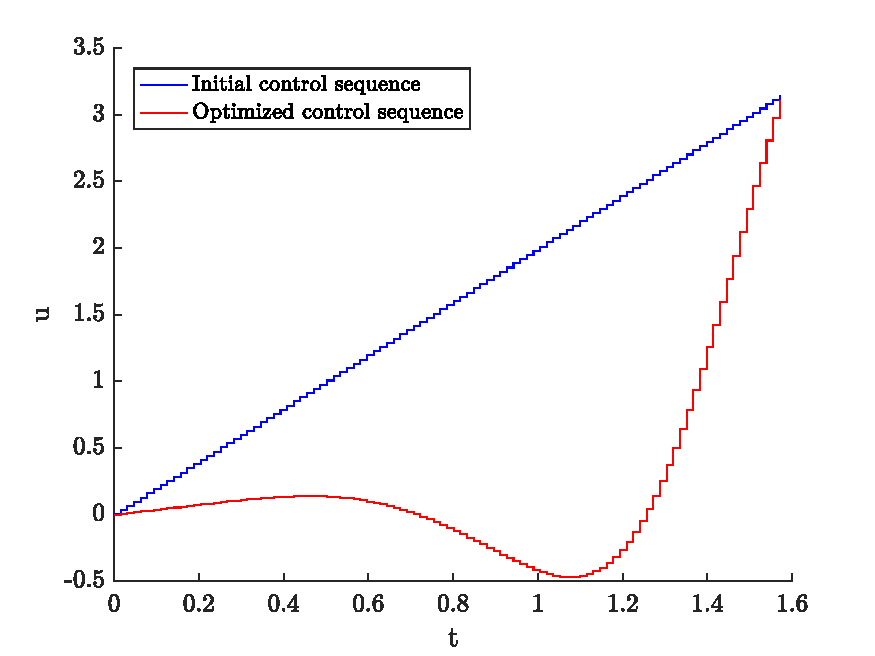
\includegraphics[width=\textwidth]{Figures/LZcontrol1.pdf}
\end{subfigure}
\hspace{3mm}
\begin{subfigure}[b]{0.48\textwidth}
	\caption{}    
  	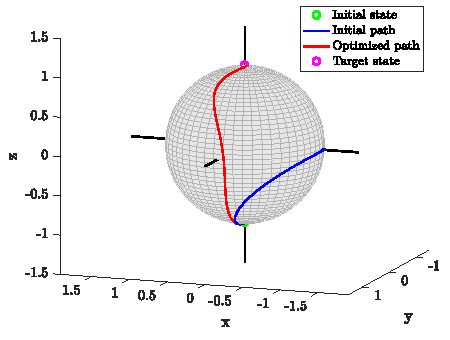
\includegraphics[width=\textwidth]{Figures/LZpath1.pdf}
\end{subfigure}

\caption{\textit{Optimal control of LZ-system using GRAPE for $T_1 = \pi / 2$. \textbf{(a)}: Initial and optimized control sequence. \textbf{(b)}: Path traced out on the Bloch sphere by the quantum state, as it is evolved according to the control.}}
\label{fig:LZopt1}
\end{figure}
Figure \ref{fig:LZopt1} displays the results of optimizing the state transfer using the GRAPE algorithm for duration $T_1 = \pi / 2$. The algorithm takes an initial linear seed, which clearly does not reach the target state. Meanwhile, the optimized control achieves perfect transfer, which is as expected, as the quantum speed limit for the transfer is $T_{\mathrm{QSL}} = T_1 = \pi / 2$, whereby a solution should exist for this duration. However, any duration shorter should not be sufficient to reach the target state.\\ 
\begin{figure}[h!]
\centering % <-- add this
\begin{subfigure}[b]{0.48\textwidth}
	\caption{}  
  	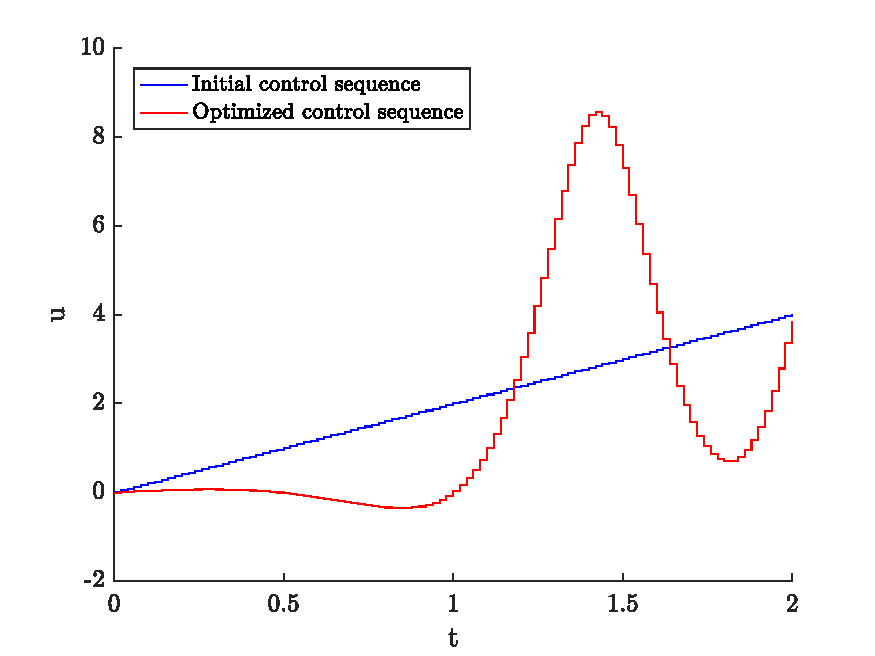
\includegraphics[width=\textwidth]{Figures/LZcontrol2.pdf}
\end{subfigure}
\hspace{3mm}
\begin{subfigure}[b]{0.48\textwidth}
	\caption{}    
  	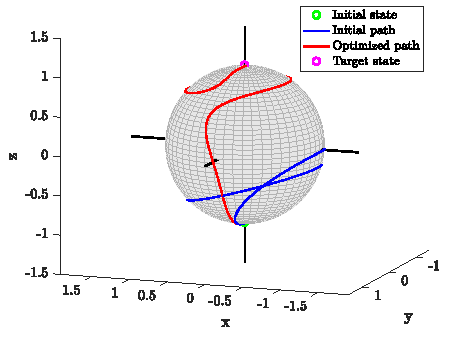
\includegraphics[width=\textwidth]{Figures/LZpath2.pdf}
\end{subfigure}

\caption{\textit{Optimal control of LZ-system using GRAPE for $T_2 = 2$. \textbf{(a)}: Initial and optimized control sequence. \textbf{(b)}: Path traced out on the Bloch sphere by the quantum state, as it is evolved according to the control.}}
\label{fig:LZopt2}
\end{figure}
Next, consider figure \ref{fig:LZopt2}, which shows the optimization results for duration $T_2 =  2$. As this duration is larger than the quantum speed limit, a solution exist for $T_2$. However, the path of the state on the Bloch sphere is much less direct than for the previous case. This is a consequence of how the optimal control problem is formulated, as one is searching for a control resulting in $\ket{\psi (T)} = \ket{\psi _{\mathrm{Target}}}$. Thus, the path of the state has no impact on the cost. Figures \ref{fig:LZopt1} and \ref{fig:LZopt2} illustrate this point, as many different paths from $\ket{\psi _0} \to \ket{\psi _{\mathrm{Target}}}$ are possible for large durations, whereas only few possible solutions are available at durations close to the quantum speed limit.

\chapter{Hessian} \label{chap:Hessian}

Consider the cost
\begin{equation}
	\mathcal{J}_T = \frac{1}{2} \left( 1- |\Braket{\psi_t | \psi (T)}|^2 \right)  = \frac{1}{2} \left( 1- \Bigg|\Braket{\psi_t | \prod_{j = 1}^{N} \hat{\mathcal{U}}_j |\psi (0)} \Bigg| ^2 \right) \; ,
\end{equation}
where the general propagator is $\hat{\mathcal{U}}_j \equiv \hat{\mathcal{U}} (u(t_j)) = \exp \{ -i \hat{H} (t_j) \Delta t \}$, and the Hamiltonian is of the form
\begin{equation}
	\hat{H}(t_j) =  \hat{H}_0 (t_j) + \sum_{n = 1}^{m}  \hat{H}_n (u_n (t_j)) \; .
\end{equation}\\
Defining the transfer probability amplitude $\mathcal{T} \equiv \braket{\psi_t | \psi (T)}$, the derivative of the cost can be formulated as
\begin{equation}
	\frac{\partial \mathcal{J}_T}{\partial u_n (t_j)} = - \frac{1}{2} \frac{\partial}{\partial u_n (t_j)}  \mathcal{T}^* \mathcal{T}   = - \Re \left( \mathcal{T}^* \frac{\partial \mathcal{T}}{\partial u_n (t_j)} \right) \; ,
\end{equation}
where
\begin{align}
	\frac{\partial \mathcal{T}}{\partial u_n (t_j)} &= \frac{\partial }{\partial u_n (t_j)} \Braket{\psi_t | \prod_{j = 1}^{N} \hat{\mathcal{U}}_j | \psi (0)} \nonumber \\
	&= \Braket{\psi_t | \hat{\mathcal{U}}_N \ldots \hat{\mathcal{U}}_{j+1} \frac{\partial \hat{\mathcal{U}}_{j}}{\partial u_n (t_j)} \hat{\mathcal{U}}_{j-1} \ldots \hat{\mathcal{U}}_{1} | \psi (0)} \nonumber \\
	&= \Braket{\psi_t (t_j) |  \frac{\partial \hat{\mathcal{U}}_{j}}{\partial u_n (t_j)}  | \psi (t_{j-1})} \; .
	\label{eq:singleDerivT}
\end{align}
The matrix elements of the cost Hessian have the form
\begin{align}
	\frac{\partial^2 \mathcal{J}}{\partial u_n (t_j) \partial u_n (t_i)} &= - \frac{1}{2} \bigg( \frac{\partial^2 \mathcal{T}}{\partial u_n (t_j)   \partial u_n (t_i)} \mathcal{T}^* + \frac{\partial \mathcal{T}}{\partial u_n (t_j)} \frac{\partial \mathcal{T}^*}{\partial u_n (t_i)} \nonumber \\
	&\qquad \quad + \frac{\partial \mathcal{T}^*}{\partial u_n (t_j)} \frac{\partial \mathcal{T}}{\partial u_n (t_i)} + \mathcal{T} \frac{\partial^2 \mathcal{T}^*}{\partial u_n (t_j)   \partial u_n (t_i)} \bigg) \nonumber \\
	&= - \Re \left( \frac{\partial \mathcal{T}}{\partial u_n (t_j)} \frac{\partial \mathcal{T}^*}{\partial u_n (t_i)} \right) - \Re \left( \frac{\partial^2 \mathcal{T}}{\partial u_n (t_j)   \partial u_n (t_i)} \mathcal{T}^* \right) \; .
\end{align}
The first term of the Hessian is easily computed from the elements of the gradient
\begin{equation}
	\frac{\partial \mathcal{T}}{\partial u_n (t_j)} \frac{\partial \mathcal{T}^*}{\partial u_n (t_i)} = \Braket{\psi_t (t_j) | \frac{\partial \hat{\mathcal{U}}_{j}}{\partial u_n (t_j)} | \psi (t_{j-1})} \Braket{\psi (t_{i-1}) | \frac{\partial \hat{\mathcal{U}}_{i}^\dag}{\partial u_n (t_i)} | \psi_t (t_{i})} \; .
\end{equation}
Meanwhile, the second term of the Hessian is more complicated, although it can easily be derived from eq. \eqref{eq:singleDerivT}
\begin{equation}
	\frac{\partial^2 \mathcal{T}}{\partial u_n (t_j) \partial u_n (t_i)} =  
	\begin{dcases}
   \Braket{\psi_t (t_j) | \frac{\partial \hat{\mathcal{U}}_{j}}{\partial u_n (t_j)}  \; \left( \prod_{k = i+1}^{j-1} \hat{\mathcal{U}}_{k}  \right) \; \frac{\partial \hat{\mathcal{U}}_{i}}{\partial u_n (t_i)}  | \psi (t_{i-1})} , & \text{for $i \neq j$}.\\
    \Braket{\psi_t (t_i) | \frac{\partial ^2 \hat{\mathcal{U}}_{j}}{\partial u_n ^2 (t_j) }   | \psi (t_{i-1})}	, & \text{for $i = j$}.
  	\end{dcases} \; .
\end{equation}
Thus, defining $\ket{\chi (T)} \equiv i \mathcal{T} \ket{\psi_t}  = i \ket{\psi_t} \braket{\psi_t | \psi (T)}$, the matrix elements of the Hessian read
\begin{align}
	\frac{\partial^2 \mathcal{J}}{\partial u_n (t_j) \partial u_n (t_i)} =& - \Re \left( \Braket{\psi_t (t_j) | \frac{\partial \hat{\mathcal{U}}_{j}}{\partial u_n (t_j)} | \psi (t_{j-1})} \Braket{\psi (t_{i-1}) | \frac{\partial \hat{\mathcal{U}}_{i}^\dag}{\partial u_n (t_i)} | \psi_t (t_{i})} \right) \nonumber \\
	&+ \Im \Braket{\chi (t_j) | \frac{\partial \hat{\mathcal{U}}_{j}}{\partial u_n (t_j)}  \; \left( \prod_{k = i+1}^{j-1} \hat{\mathcal{U}}_{k}  \right) \; \frac{\partial \hat{\mathcal{U}}_{i}}{\partial u_n (t_i)}  | \psi (t_{i-1})} (1 - \delta_{i , j}) \nonumber \\
	&+ \Im 	 \Braket{\chi (t_i) | \frac{\partial ^2 \hat{\mathcal{U}}_{j}}{\partial u_n ^2 (t_j) }   | \psi (t_{i-1})} \delta_{i , j} \; .
	\label{eq:generalHessianElements}
\end{align}


\subsubsection{Hessian for Suzuki-Trotter Propagator}
Consider the case where the control Hamiltonians, $\hat{H}_n$, are diagonal, whereby they and their derivatives mutually commute. Expanding the propagator through the Suzuki-Trotter expansion and evaluating the control function at each end of the time-step interval produces the propagator 
\begin{equation}
	\hat{\mathcal{U}}_{j}^{\mathrm{ST}} = \left( \prod_{n = 1}^{m} e^{ -i \hat{H}_n (t_j) \Delta t /2 } \right) \: e^{ -i \hat{H}_0 \Delta t } \: \left( \prod_{n = 1}^{m} e^{  -i  \hat{H}_n  (t_{j-1})  \Delta t /2 } \right) \; .
\end{equation}
The derivative of the Suzuki-Trotter propagator is
\begin{equation}
	\frac{\partial \hat{\mathcal{U}}_{k}^{\mathrm{ST}}}{\partial u_n (t_j)} = \left( -i \frac{\partial \hat{H}_n (t_j)}{\partial u_n (t_j)} \frac{\Delta t}{2} \right) \hat{\mathcal{U}}_{j}^{\mathrm{ST}} \delta_{j , k} + \hat{\mathcal{U}}_{j}^{\mathrm{ST}} \left( -i \frac{\partial \hat{H}_n (t_{j-1})}{\partial u_n (t_{j-1})} \frac{\Delta t}{2} \right)  \delta_{j , k+1} \; ,
\end{equation}
where the two contributions origin from the end-point evaluation of the control. Thus, the derivatives with respect to $u_n (t_j)$ stated above will have contributions from both $\hat{\mathcal{U}}_{j}^{\mathrm{ST}}$ and $\hat{\mathcal{U}}_{j+1}^{\mathrm{ST}}$. Thereby the first order derivative of the transfer probability amplitude reads 
\begin{equation}
	\frac{\partial \mathcal{T}^{\mathrm{ST}}}{\partial u_n (t_j)} = -i \Delta t \Braket{\psi_t (t_j) | \frac{\partial \hat{H}_n (t_j)}{\partial u_n (t_j)} | \psi (t_j) } \; ,
\end{equation}
from which the second order derivative can be calculated. Starting with the case $i \neq j$, the contributions to the derivative from two propagators results in
\begin{align}
	\frac{\partial^2 \mathcal{T}^{\mathrm{ST}}}{\partial u_n (t_j) \partial u_n (t_i)} =& -i \Delta t \Braket{\psi_t (t_{i+1}) | \frac{\partial \hat{\mathcal{U}}_{i+1}^{\mathrm{ST}}}{\partial u_n (t_i)} \; \left( \prod_{k = j+1}^{i} \hat{\mathcal{U}}_{k}^{\mathrm{ST}} \right) \; \frac{\partial \hat{H}_n (t_j)}{\partial u_n (t_j)} | \psi (t_j) } \nonumber \\
	& -i \Delta t \Braket{\psi_t (t_{i}) | \frac{\partial \hat{\mathcal{U}}_{i}^{\mathrm{ST}}}{\partial u_n (t_i)} \; \left( \prod_{k = j+1}^{i-1} \hat{\mathcal{U}}_{k}^{\mathrm{ST}} \right) \; \frac{\partial \hat{H}_n (t_j)}{\partial u_n (t_j)} | \psi (t_j) } \nonumber \\
	=& -i \Delta t \Braket{\psi_t (t_{i+1}) |  \hat{\mathcal{U}}_{i+1}^{\mathrm{ST}} \left( -i \frac{\partial \hat{H}_n (t_i)}{\partial u_n (t_i)} \frac{\Delta t}{2} \right) \; \left( \prod_{k = j+1}^{i} \hat{\mathcal{U}}_{k}^{\mathrm{ST}} \right) \; \frac{\partial \hat{H}_n (t_j)}{\partial u_n (t_j)} | \psi (t_j) } \nonumber \\
	& -i \Delta t \Braket{\psi_t (t_{i}) | \left( -i \frac{\partial \hat{H}_n (t_i)}{\partial u_n (t_i)} \frac{\Delta t}{2} \right) \hat{\mathcal{U}}_{i}^{\mathrm{ST}} \; \left( \prod_{k = j+1}^{i-1} \hat{\mathcal{U}}_{k}^{\mathrm{ST}} \right) \; \frac{\partial \hat{H}_n (t_j)}{\partial u_n (t_j)} | \psi (t_j) } \nonumber \\
	=& - \Delta t^2 \Braket{\psi_t (t_i) | \frac{\partial \hat{H}_n (t_i)}{\partial u_n (t_i)} \left( \prod_{k = j + 1}^{i} \hat{\mathcal{U}}_{k}^{\mathrm{ST}} \right) \frac{\partial \hat{H}_n (t_j)}{\partial u_n (t_j)} | \psi (t_j) }  \; .
\end{align}
The case of $i = j$ included an extra term, as one must remember the derivative of ${\partial \hat{H}_n (t_j)}/{\partial u_n (t_j)}$. Thereby the second order derivative reads
\begin{align}
	\frac{\partial^2 \mathcal{T}^{\mathrm{ST}}}{\partial u_n ^2 (t_j)} =& -i \Delta t \Braket{\psi_t (t_{j+1}) | \frac{\partial \hat{\mathcal{U}}_{j+1}^{\mathrm{ST}}}{\partial u_n (t_j)} \frac{\partial \hat{H}_n (t_j)}{\partial u_n (t_j)} | \psi (t_j) } \nonumber \\
 & 	-i \Delta t \Braket{\psi_t (t_{j}) |  \frac{\partial ^2 \hat{H}_n (t_j)}{\partial u_n ^2(t_j)} | \psi (t_j) } \nonumber \\
 & -i \Delta t \Braket{\psi_t (t_{j}) |  \frac{\partial \hat{H}_n (t_j)}{\partial u_n (t_j)} \frac{\partial \hat{\mathcal{U}}_{j}^{\mathrm{ST}}}{\partial u_n (t_j)}| \psi (t_{j-1}) } \nonumber \\
 & = - i \Delta t \Braket{\psi_t (t_i) | \frac{\partial^2 \hat{H}_n (t_j)}{\partial u_n ^2 (t_j)} - i \Delta t \left( \frac{\partial \hat{H}_n (t_j)}{\partial u_n (t_j)} \right)^2 | \psi (t_j) } \; .
\end{align}
Thus, the second order derivatives of the transfer probability amplitude can be summarized as 
\begin{equation}
	\frac{\partial^2 \mathcal{T}^{\mathrm{ST}}}{\partial u_n (t_j) \partial u_n (t_i)} =  
	\begin{dcases}
   - \Delta t^2 \Braket{\psi_t (t_i) | \frac{\partial \hat{H}_n (t_i)}{\partial u_n (t_i)} \left( \prod_{k = j + 1}^{i} \hat{\mathcal{U}}_{k}^{\mathrm{ST}} \right) \frac{\partial \hat{H}_n (t_j)}{\partial u_n (t_j)} | \psi (t_j) } , & \text{for $i \neq j$}.\\
    - i \Delta t \Braket{\psi_t (t_i) | \frac{\partial^2 \hat{H}_n (t_j)}{\partial u_n ^2 (t_j)} - i \Delta t \left( \frac{\partial \hat{H}_n (t_j)}{\partial u_n (t_j)} \right)^2 | \psi (t_j) }	, & \text{for $i = j$}.
  	\end{dcases} \; .
\end{equation} 
Inserting the propagator into the elements of the Hessian \eqref{eq:generalHessianElements} produces 
\begin{align}
	\frac{\partial^2 \mathcal{J}}{\partial u_n (t_j) \partial u_n (t_i)} =& - \Re \left( \Braket{\psi_t (t_j) | \frac{\partial \hat{H}_n  (t_j)}{\partial u_n (t_j)} | \psi (t_{j})} \Braket{\psi (t_{i}) | \frac{\partial \hat{H}_n  (t_i)}{\partial u_n (t_i)} | \psi_t (t_{i})} \right) \Delta t ^2 \nonumber \\
	&- \Im \Braket{\chi (t_j) | \frac{\partial \hat{H}_n  (t_j)}{\partial u_n (t_j)}  \; \left( \prod_{k = i+1}^{j} \hat{\mathcal{U}}_{k}^{\mathrm{ST}}  \right) \; \frac{\partial \hat{H}_n (t_i)}{\partial u_n (t_i)}  | \psi (t_{i})} \Delta t^ 2  ( 1 - \delta_{i , j}) \nonumber \\
	&- \Re \Braket{\chi (t_i) | \frac{\partial^2 \hat{H}_n (t_j)}{\partial u_n ^2 (t_j)} - i \Delta t \left( \frac{\partial \hat{H}_n (t_j)}{\partial u_n (t_j)} \right)^2 | \psi (t_j) } \Delta t \delta_{i,j} \; .
	\label{eq:expandedHessianElements}
\end{align}
Having already computed the elements of the gradient, the number of step-propagations needed for the computation of the full Hessian is $N^2 / 2 - N$ due to the symmetry of the matrix and the lack of new propagations for computing the diagonal elements.

%----------------------------------------------------------------------------------------

\end{document}  
